%%%%%%%% ICML 2026 EXAMPLE LATEX SUBMISSION FILE %%%%%%%%%%%%%%%%%

\documentclass{article}

% Recommended, but optional, packages for figures and better typesetting:
\RequirePackage{graphicx}
\usepackage{microtype}
\usepackage{graphicx}
\usepackage{subfigure}
\usepackage{booktabs}
\usepackage[shortlabels]{enumitem}
\usepackage{pifont}
\usepackage[dvipsnames]{xcolor}
\newcommand{\theHalgorithm}{\arabic{algorithm}}
\RequirePackage{fancyhdr}
\RequirePackage{xcolor}
\RequirePackage{algorithm}
\RequirePackage[noend]{algorithmic}
\RequirePackage{natbib}
\RequirePackage{eso-pic}
\RequirePackage{forloop}
\RequirePackage{url}
% please comment out the following usepackage line and replace
% \usepackage{icml2025} with \usepackage[nohyperref]{icml2025} above.
\usepackage{hyperref}
\usepackage{booktabs}
\usepackage{amsmath,amssymb,amsthm}
\usepackage{soul}
\usepackage{subcaption}
\usepackage{multirow}
\usepackage{mathtools}
\usepackage{amsthm}
\usepackage[thinc]{esdiff}
\usepackage[table]{xcolor}
\definecolor{red}{rgb}{1.0000,0.5686,0.5059}
\definecolor{orange}{rgb}{1.0000,0.7373,0.5059}
\definecolor{yellow}{rgb}{0.9176, 0.9098, 0.4353}
\definecolor{red1}{rgb}{0.921569, 0.282353, 0.247059}
\definecolor{green1}{rgb}{0.501961, 0.792157, 0.239216}
\definecolor{orange1}{rgb}{0.937255, 0.529412, 0.2}
\usepackage{longtable}
\usepackage[capitalize,noabbrev]{cleveref}
\usepackage[textsize=tiny]{todonotes}
\makeatletter
\def\set@curr@file#1{\def\@curr@file{#1}}
\makeatother
\usepackage[load-configurations=version-1]{siunitx}

% hyperref makes hyperlinks in the resulting PDF.
% If your build breaks (sometimes temporarily if a hyperlink spans a page)
% please comment out the following usepackage line and replace
% \usepackage{icml2026} with \usepackage[nohyperref]{icml2026} above.
\usepackage{hyperref}


% Attempt to make hyperref and algorithmic work together better:
%\newcommand{\theHalgorithm}{\arabic{algorithm}}

% Use the following line for the initial blind version submitted for review:
%\usepackage{icml2026}
\usepackage{xspace}
% For preprint, use
%\usepackage[preprint]{icml2026}

% If accepted, instead use the following line for the camera-ready submission:
\usepackage[accepted]{icml2026}

% if you use cleveref..
\usepackage[capitalize,noabbrev]{cleveref}

%%%%%%%%%%%%%%%%%%%%%%%%%%%%%%%%
% THEOREMS
%%%%%%%%%%%%%%%%%%%%%%%%%%%%%%%%
\theoremstyle{plain}
\newtheorem{theorem}{Theorem}[section]
\newtheorem{proposition}[theorem]{Proposition}
\newtheorem{lemma}[theorem]{Lemma}
\newtheorem{corollary}[theorem]{Corollary}
\theoremstyle{definition}
\newtheorem{definition}[theorem]{Definition}
\newtheorem{assumption}[theorem]{Assumption}
\theoremstyle{remark}
\newtheorem{remark}[theorem]{Remark}

% Todonotes is useful during development; simply uncomment the next line
%    and comment out the line below the next line to turn off comments
%\usepackage[disable,textsize=tiny]{todonotes}
\usepackage[textsize=tiny]{todonotes}

% The \icmltitle you define below is probably too long as a header.
% Therefore, a short form for the running title is supplied here:
\icmltitlerunning{LiLAW: Lightweight Learnable Adaptive Weighting}

\begin{document}

\twocolumn[
  \icmltitle{LiLAW: Lightweight Learnable Adaptive Weighting \\ \vspace{0.1em} to Meta-Learn Sample Difficulty, Improve Noisy Training, \\ Increase Fairness, and Effectively Use Synthetic Data}

  % It is OKAY to include author information, even for blind submissions: the
  % style file will automatically remove it for you unless you've provided
  % the [accepted] option to the icml2026 package.

  % List of affiliations: The first argument should be a (short) identifier you
  % will use later to specify author affiliations Academic affiliations
  % should list Department, University, City, Region, Country Industry
  % affiliations should list Company, City, Region, Country

  % You can specify symbols, otherwise they are numbered in order. Ideally, you
  % should not use this facility. Affiliations will be numbered in order of
  % appearance and this is the preferred way.
  \icmlsetsymbol{equal}{*}

  \begin{icmlauthorlist}
    \icmlauthor{Abhishek Moturu}{cs,v,sk,kite}
    \icmlauthor{Muhammad Muzammil}{cs,kite}
    \icmlauthor{Anna Goldenberg}{cs,v,sk,lmp}
    \icmlauthor{Babak Taati}{cs,kite}
    %\icmlauthor{}{sch}
    %\icmlauthor{}{sch}
  \end{icmlauthorlist}

  \icmlaffiliation{cs}{Department of Computer Science, University of Toronto, Ontario, Canada}
  \icmlaffiliation{lmp}{Department of Laboratory Medicine \& Pathobiology, University of Toronto, Ontario, Canada}
  \icmlaffiliation{v}{Vector Institute, Ontario, Canada}
  \icmlaffiliation{sk}{The Hospital for Sick Children, Ontario, Canada}
  \icmlaffiliation{kite}{UHN KITE Research Institute, Ontario, Canada}

  \icmlcorrespondingauthor{Abhishek Moturu}{moturuab@cs.toronto.edu}
  %\icmlcorrespondingauthor{Firstname2 Lastname2}{first2.last2@www.uk}

  % You may provide any keywords that you find helpful for describing your
  % paper; these are used to populate the "keywords" metadata in the PDF but
  % will not be shown in the document
  \icmlkeywords{Machine Learning, ICML}

  \vskip 0.3in
]

% this must go after the closing bracket ] following \twocolumn[ ...

% This command actually creates the footnote in the first column listing the
% affiliations and the copyright notice. The command takes one argument, which
% is text to display at the start of the footnote. The \icmlEqualContribution
% command is standard text for equal contribution. Remove it (just {}) if you
% do not need this facility.

\newcommand{\synpain}{Syn\textsc{Pain}\xspace}
\newcommand{\gaitgen}{\textsc{Gait}Gen\xspace}

% Use ONE of the following lines. DO NOT remove the command.
% If you have no special notice, KEEP empty braces:
\printAffiliationsAndNotice{}  % no special notice (required even if empty)
% Or, if applicable, use the standard equal contribution text:
% \printAffiliationsAndNotice{\icmlEqualContribution}

\begin{abstract}
Training deep neural networks with noise and data heterogeneity is a major challenge. We introduce Lightweight Learnable Adaptive Weighting (LiLAW), a method that dynamically adjusts the loss weight of each training sample based on its evolving difficulty, categorized as easy, moderate, or hard. Using only three learnable parameters, LiLAW adaptively prioritizes informative samples during training by updating these parameters using a single gradient descent step on a validation mini-batch after each training mini-batch.
%, without excessive tuning.
%requiring excessive hyperparameter tuning or a clean validation set. 
Experiments across multiple general and medical imaging datasets, noise levels/types, loss functions, and architectures with and without pretraining (with linear probing and full fine-tuning) demonstrate that LiLAW's effectiveness, even in high-noise environments, without excessive tuning. 
%We also provide extensions for LiLAW in the multi-label classification and regression settings. 
We also apply LiLAW to two recently introduced synthetic datasets: \synpain (synthetic facial expressions for automated pain detection) and \gaitgen (synthetic gait sequences for Parkinson's disease severity estimation). We also validate on ECG5000, a time-series dataset for heartbeat classification, with simple augmentations. We obtain state-of-the-art results on these three datasets. We then use LiLAW on the Adult dataset to show improved fairness. LiLAW is effective without heavy reliance on advanced training techniques or data augmentations, highlighting its practicality, esp. in resource-constrained settings. It offers a computationally efficient solution to boost generalization and robustness in any neural network training setup. %\footnote{Code in Supplementary Material.}

% TALK ABOUT resource constrained environments
% SAY that we can identify noise well in the training data
\end{abstract}
%\vspace{-1em}
\section{Introduction}
\label{sec:introduction}

The increasing availability of very large labeled datasets has played a major role in advancing machine learning and computer vision in recent years. However, imaging datasets often contain samples with varying levels of quality, affecting the efficiency and effectiveness of model training. This issue is particularly significant in medical imaging datasets, which typically have smaller sample sizes, exhibit greater heterogeneity, and often require specialized expertise for accurate labeling. Ensuring that models make the best use of a small amount of noisy, heterogeneous data remains a key challenge, as not all samples are equally informative or beneficial for model performance. At varying rates at different points during training, samples can benefit the model, hurt the model, or not affect the model much at all.

Several methods have been proposed to quantify the difficulty or importance of individual samples~\citep{agarwal_estimating_2022, paul2021deep, baldock2021deep, maini2022characterizing, siddiqui2022metadata, rabanser2022selective, toneva2018empirical, pliushch2022deep, xu_understanding_2021, kong_adaptive_2021, dong2023generalized, jiang2020characterizing, seedat_dissecting_2024}. Understanding which samples a model finds difficult to predict is essential for safe model deployment, sample selection for human-in-the-loop auditing, and gaining insights into model behavior~\citep{agarwal_estimating_2022}. Knowing or estimating example difficulty can help separate misclassified, mislabeled, and rare examples~\citep{maini2022characterizing}, prune data~\citep{paul2021deep}, quantify uncertainty~\citep{dong2023generalized}, improve generalization~\citep{xu_understanding_2021}, increase convergence speed~\citep{kong_adaptive_2021}, enhance out-of-distribution detection~\citep{agarwal_estimating_2022}, and provide insights into example memorization and forgetting~\citep{toneva2018empirical}. While existing methods provide insights into individual data points and how models learn, they often do not adjust the training process in a dynamic, efficient manner. This may restrict potential improvements in model performance, robustness, and generalization.

Focusing on the most relevant data at different stages of training can help leverage datasets effectively. A common limitation in many existing approaches is the static or uniform treatment of all data points during training. Standard practice does not apply additional weights to samples or take sample difficulty into account. Existing sample weighting methods usually require a clean validation set, a separate model to learn sample difficulty, and/or a higher training complexity (see Sec.~\ref{sec:sampleweighting}).

In this paper, we propose a novel method called \textbf{Li}ghtweight \textbf{L}earnable \textbf{A}daptive \textbf{W}eighting (\textbf{LiLAW}), which addresses these challenges with a lightweight, adaptive mechanism to adjust the weight of each sample's loss based on its difficulty. Our approach introduces a simple yet powerful parametrization, using three parameters pertaining to learning easy, moderate, and hard samples (see Figure \ref{fig:diagram}). These parameters are used to calculate the weight of each sample loss and are jointly optimized with a single gradient descent step on the validation set after every training mini-batch.

\begin{figure}
    \centering
    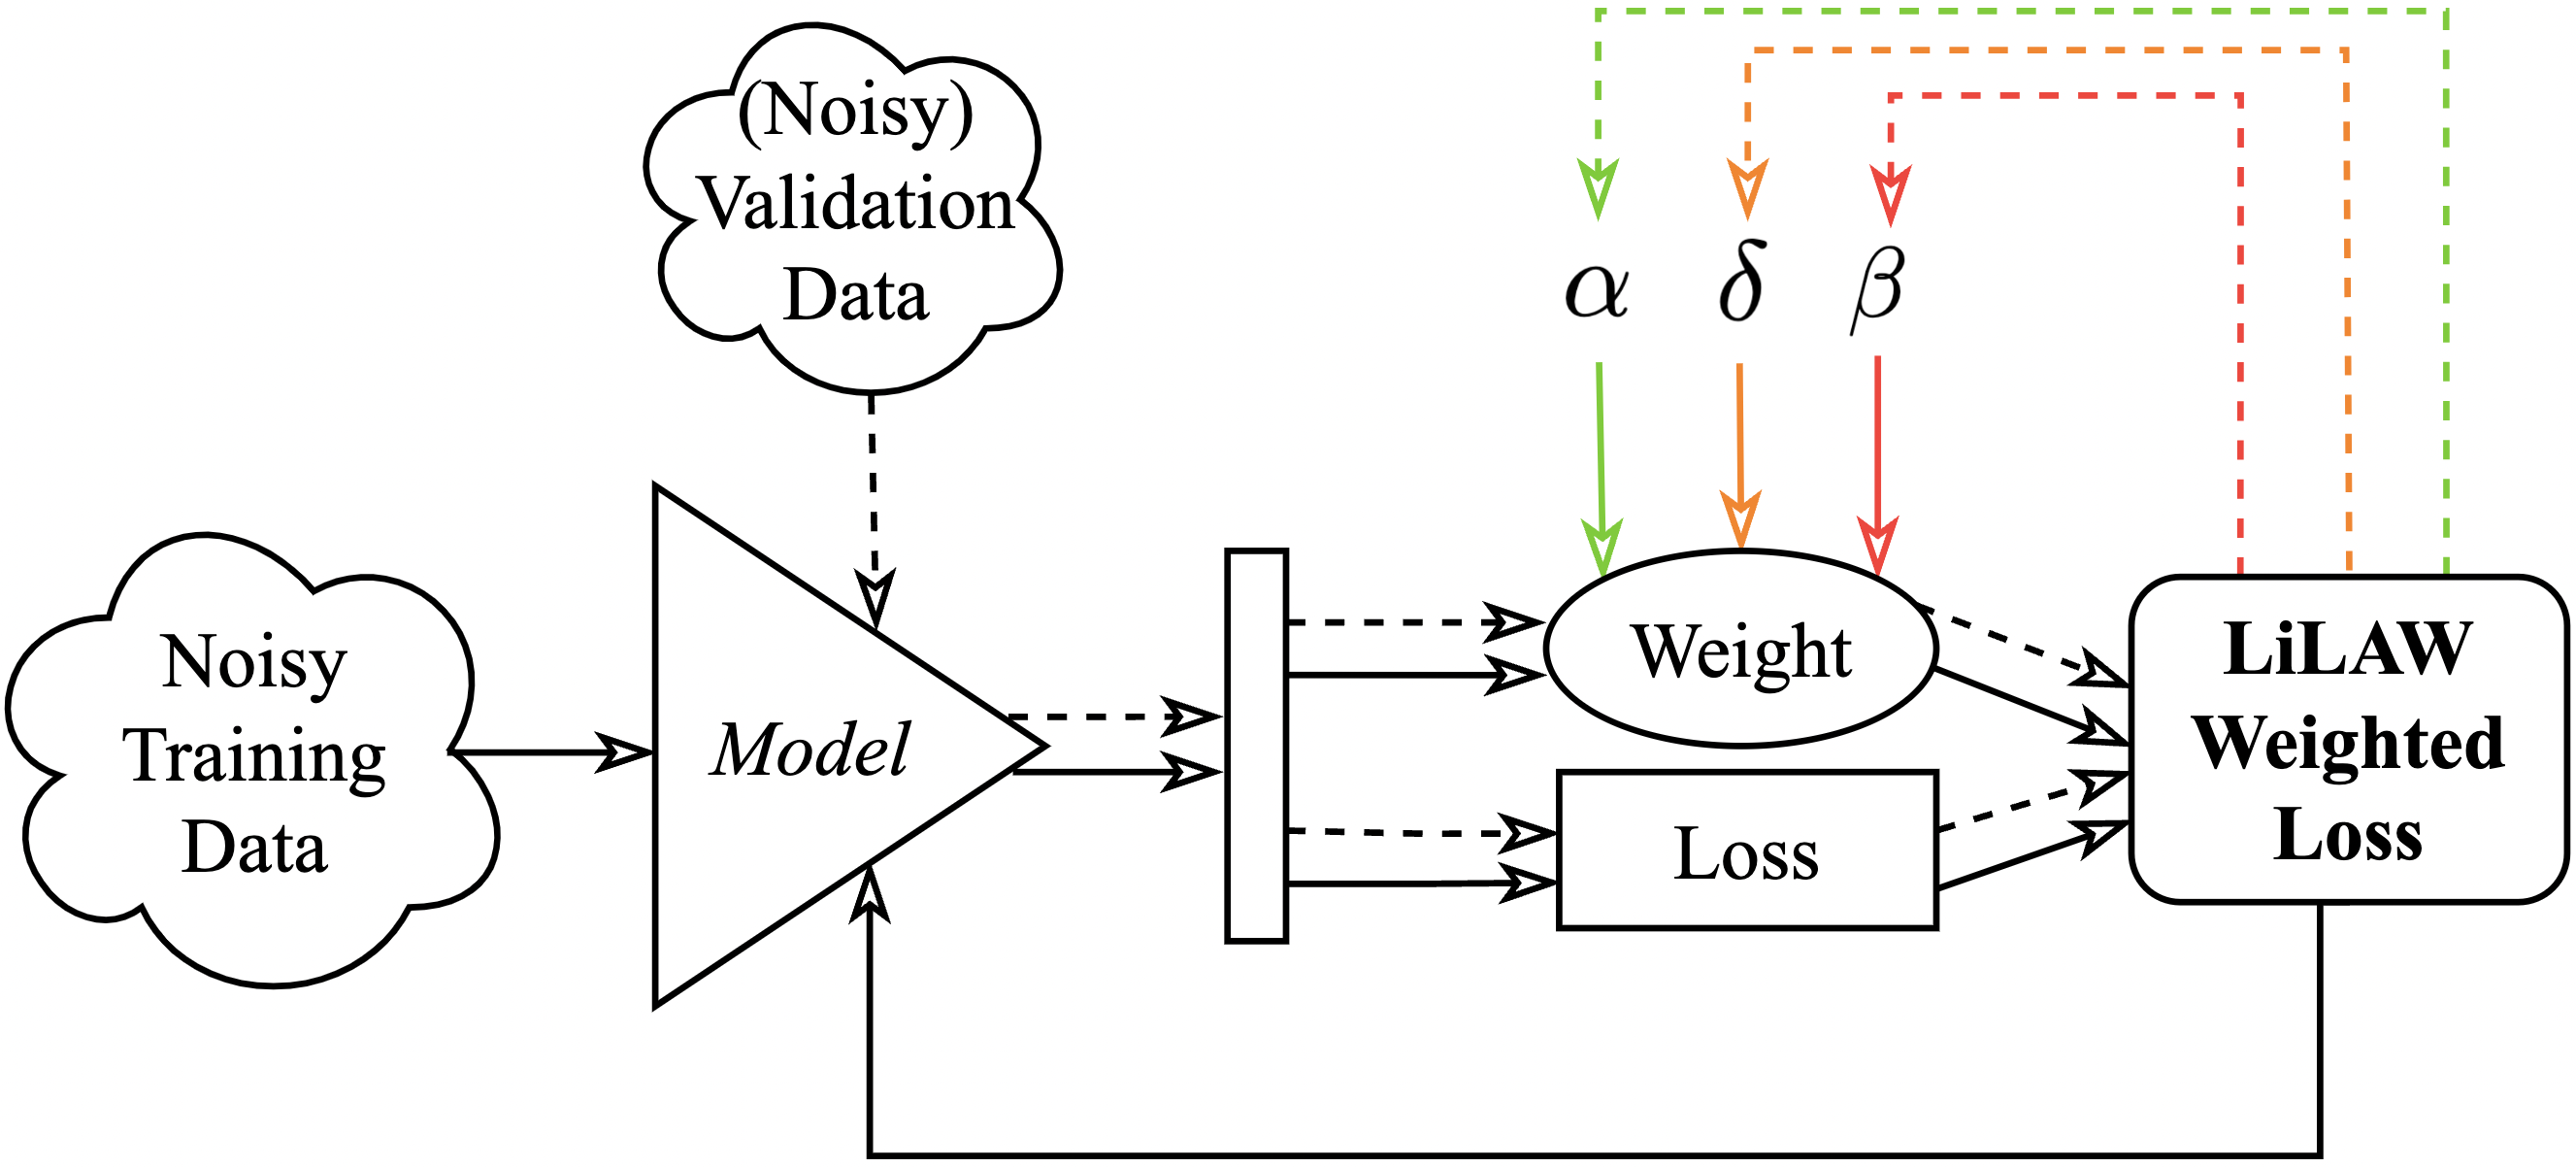
\includegraphics[scale=0.142]{diagram.png}
    \caption{Given noisy training and validation data, LiLAW learns to adaptively weight the loss of each sample based on three trainable parameters, $\alpha, \delta, \beta$, pertaining to learning \textcolor{green1}{easy}, \textcolor{orange1}{moderate}, and \textcolor{red1}{hard} samples, respectively, at different stages of training using meta-learning on the validation data.}
    \label{fig:diagram}
\end{figure}

Importantly, our method does not require a clean, unbiased validation set. Unlike static weighting schemes or hyperparameter-based weighting search schemes, LiLAW learns to adaptively prioritize different samples as training progresses. By integrating sample difficulty assessments into the training process, LiLAW helps the model focus on the most informative data when it is most beneficial, while maintaining computational efficiency.

We first introduce our theoretical framework and then perform extensive experiments with and without LiLAW in various settings to show its effectiveness. 

%Our results show that LiLAW improves test performance across several general and medical imaging datasets, models, loss functions, noise types, noise levels, with and without pretraining, with and without calibration, and with and without a clean and unbiased validation set. This is done without the need for excessive hyperparameter tuning and without increasing the time and space complexity. 

In summary, we introduce a new method, LiLAW, that:
\vspace{-1em}
\begin{enumerate}[leftmargin=*,labelindent=0pt,label=\textbf{--}]
    \itemsep-0.4em 
    \item only adds three extra trainable parameters and does not require more models for difficulty-learning or pruning (easy-to-implement, maintains similar space complexity);
    \item only needs one additional forward and backward pass on a single validation mini-batch after each training mini-batch (maintains similar time complexity);
    \item uses weighting to measure difficulty, inform model training, and improve test performance without pruning (identifies noisy samples, avoids further reducing dataset size);
    \item uses meta-learning to avoid extensive hyperparameter tuning (saves time, useful in resource-constrained settings);
    \item does not require a clean, unbiased meta-validation set (may be hard to obtain in some domains);
    %\item works when training from scratch, linear probing, or full fine-tuning;
    \item provably improves noisy learning when there is diagonally dominant label noise;
    \item provably reduces disparities to improve fairness;
    \item offers an intuitive graphical and mathematical understanding of the weighting; and,
    \item is adaptive, lightweight, and easy-to-implement on top of any model training or fine-tuning.
\end{enumerate}

\section{Related Work}
\label{sec:relatedwork}

The effectiveness of machine learning models, especially deep neural networks, is highly dependent on the quality and proper use of training data. Recent literature has explored strategies to improve model performance and robustness to address challenges presented by noisy, mislabeled, underrepresented, or otherwise hard-to-learn data.

\subsection{Data-Centric AI}

\citet{pleiss_identifying_2020} proposed using the area under the margin ranking to identify mislabeled data and improve model performance by filtering out mislabeled data, which requires ``dataset cleaning.''
\citet{toneva2018empirical} conducted an empirical study on example forgetting during deep neural network training that shed light on data quality highlighting that some samples that are forgotten frequently, some are not forgotten at all, and some could be omitted from training without affecting the model greatly. \citet{paul2021deep} highlight that simple scores such as the Gradient Normed (GraNd) and Error L2-Norm (EL2N) can be used to identify important examples very early in training and to prune significant portions of the training data while maintaining test accuracy. \textit{Our method instead aims to improve test performance without pruning any training data.}

\citet{wu_learning_2023} presented a framework for selecting pivotal samples for meta re-weighting, aiming to optimize performance on a small set of perfect samples, which may not be available in many real-world cases. \citet{mindermann_prioritized_2022} note that a lot of samples may be hard to learn since they are noisy or unlearnable. They propose a method that selects points that are learnable, worth learning, and not yet learnt. However, this method requires a separate small model trained on a holdout set. \textit{Our method does not require a clean, unbiased meta-validation set or a separate model.}


\citet{agarwal_estimating_2022} propose estimating example difficulty using variance of gradients to rank data by hardness and identify samples for auditing. \citet{swayamdipta_dataset_2020} present a method to map datasets using training dynamics to identify easy, hard, and ambiguous examples. These methods do not use difficulty information to inform training. \textit{Our method serves both to assess sample difficulty and to use that information to enhance training.}

\citet{jia_learning_2022} use raw training dynamics as input to an LSTM noise detector network which learns to predict mislabels. 
\citet{jiang_delving_2021} use loss curves to identify corrupted labels and tailed classes by training a whole network on the original data and then training a CurveNet on the loss curves of each sample as an additional attribute to identify bias type. These methods and others \citep{dividemix,topological,unicon,combatingsurrogate} require additional models for difficulty-learning or data selection. \textit{Our method does not require additional models.}

In addition, accurate uncertainty estimation and model calibration are essential for reliable predictions. Models are well-calibrated if predicted probabilities accurately reflect the chance of an event occurring. \citet{guo_calibration_2017} investigated the calibration of neural networks and found that deeper networks are often poorly calibrated. They propose temperature scaling as an effective calibration method. Another approach to improve calibration is label smoothing \citep{muller_when_2020}. \textit{Our method works synergistically with calibration to improve model performance.}

Several methods were developed to characterize sample hardness and data quality such as Data-IQ (Data-Inherent Qualities)~\cite{seedat_data-iq_2022}, DIPS (Data-centric Insights for Pseudo-labeling with Selection)~\cite{seedat_you_2024}, and H-CAT (Hardness Characterization Analysis Toolkit)~\cite{seedat_dissecting_2024}. We use H-CAT to study the effectiveness of our method across various settings.

\subsection{Sample Weighting}
\label{sec:sampleweighting}
Sample weighting aims to improve model training by assigning weights to samples based on their learning difficulty. Traditional methods often rely on static weighting schemes, which fail to adapt to a model's evolving learning dynamics. Several works introduced a theoretical framework connecting generalization error to difficulty \citep{zhou_which_2023, zhou_understanding_2023, zhu_exploring_2022}. \citet{zhou_which_2023} propose adaptive weighting strategies that consider easy, moderate, and hard samples and use hyperparameter tuning to find the most effective weighting solution, which stays fixed, from easy-first, hard-first, medium-first, and two-ends-first or a pre-defined schedule (easy-first, then hard-first) during training. \textit{Our method adaptively prioritize different samples as training progresses.}

\citet{xu_understanding_2021} mention that using counterfactual modeling to jointly train a weighting model with the classifier eventually causes the weights to converge to the same constant. Other methods state that increasing weights on hard samples may improve both convergence and performance, but assume that training noise is absent~\citep{zhou_understanding_2023, xu_understanding_2021}. \textit{Our method assumes that training label noise may exist and does not require extensive hyperparameter tuning to find the best learning strategy.}

Meta-learning aims to improve the learning process itself. It is often referred to as ``learning to learn'' in literature. Recent work has shown promise in using meta-learning to learn weights for samples. %\citet{wu_revisiting_2024} propose a theoretical framework for sample weighting based on the effective number theory for imbalanced learning using meta-learning, which usually requires an unbiased meta-set.
To aid in learning to select the samples for the meta-set, \citet{jain_improving_2024} employ a bi-level objective aimed at identifying the most challenging samples in the training data to use as a validation set and subsequently train the classifier to reduce errors on those specific samples, which is a way of learning a Learned Reweighting (LRW) classifier without a fixed, unbiased, and clean validation set~\citep{ren_learning_2019}. However, this requires three networks: one to learn the task, one that identifies challenging samples to validate, and one that learns sample weights, vastly increasing computational complexity. \textit{Our method only requires three additional trainable global parameters.}

Methods like probabilistic margin~\citep{wang_probabilistic_2022} and area under the margin~\citep{pleiss_identifying_2020} measure the difference between the score of the observed label in the softmax of the logits of the neural network and the maximum score in the softmax (discounting the score of the observed label). The range of possible negative values makes it difficult to use these methods in loss-based weighting schemes. \textit{In contrast, our method guarantees reasonable positive weights.}

\citet{kong_adaptive_2021} propose adaptive (as opposed to fixed) curriculum learning which uses the current model to adjust loss-based difficulty scores while retaining learned knowledge from a pre-trained model using the KL divergence between the outputs of the current model and the pre-trained model and a pacing function to control the learning pace. This assumes the existence of a pre-trained network for the task at hand. \textit{Our method does not require additional models and only needs one additional forward and backward pass to do a single gradient descent step on a validation mini-batch after every training mini-batch.}

\subsection{Synthetic Data Generation}
Synthetic data generation methods include Generative Adversarial Networks (GANs)~\citep{gan}, Variational Autoencoders (VAEs)~\citep{vae}, and diffusion models~\citep{diffusion}, and help address data scarcity, privacy issues, and demographic imbalance~\citep{bauer2024comprehensive}. GANs (StyleGAN~\citep{stylegan1,stylegan2}, Progressive GAN~\citep{pggan}) have synthesized high-fidelity images but struggle with diversity and mode collapse. VAEs have also been successful in data generation with controlled latent variables but typically achieve lower fidelity compared to GANs. Diffusion models have achieved very high fidelity compared to GANs and VAEs by starting with random noise and learning to denoise to generate high-quality data. They are usually combined with text-encoders to allow for text prompts~\cite{zhang2024texttoimagediffusionmodelsgenerative}, but may be unable to fully capture physiological or biological data.

Recent methods, such as \synpain~\cite{taati2025synpain}, address these limitations with a diverse synthetic dataset specifically designed for pain classification, thus overcoming demographic bias prevalent in traditional datasets. Similarly, \gaitgen~\cite{adeli2025gaitgen} introduces clinically relevant synthetic gait data conditioned on pathological severity, addressing the scarcity of high-quality labeled clinical data and underrepresentation of severe pathology cases. Despite this, synthetic datasets need to be handled carefully due to variability in generation quality and distributional discrepancies with real data. Incorporating synthetic data does not always improve performance. \textit{Our method helps effectively use synthetic data and data augmentations during training.} %These issues are not fully addressed by standard data augmentation methods.

\subsection{Reweighting for Fairness}

Reweighting is also used as a lightweight method to improve fairness since it can give different training samples different importance in the loss. Early methods assigned weights to groups and labels proportionally during pre-processing~\citep{kamiran}, however later methods have made reweighting adaptive to better satisfy fairness objectives while training~\citep{krasanakis, chai}. More recent methods aim to achieve better fairness through meta-learning, where weights are optimized jointly with the model parameters~\citep{yan2020forml}. \textit{Our method also assigns meta-learned adaptive weights to each sample's loss and improves fairness across subgroups.}

\section{Method}
\label{sec:method}

Consider the following supervised multi-class classification problem setup used in prior work~\citep{northcutt_confident_2022}.
% 
Let $\mathcal{D}_{t} = \{(x_i, \widetilde{y_i})\}^N_{i=1}$ represent the training set and $\mathcal{D}_{v} = \{(x_j, \widetilde{y_j})\}^{N+M}_{j=N+1}$ represent the validation set. Note that $(x_i, \widetilde{y_i})$ represents the pairs of inputs and observed (potentially noisy) targets. Specifically, $x_i \in \mathcal{X}$, where $\mathcal{X}$ is the input space (e.g.: images) and $\widetilde{y_i} \in \mathcal{Y} = \{0,...,c-1\},$ is the output space with $c \in \mathbb{N}$ such that $c \ge 2$ is the total number of classes. Note that $\widetilde{y_i}$ is a single integer value, i.e. $x_i$ belongs to a single class. Let $y_i \in \mathcal{Y}$ be the true target. Let $f_{\theta}: \mathcal{X} \rightarrow \mathcal{Y}$ be the neural network model, $\theta$ be its parameters, and $s_i = \mathrm{softmax}(f_{\theta}(x_i))$ be the softmax of its logits. Therefore, $s_i \in \mathbb{R}^c$ such that $\sum_{j=0}^{c-1} s_i[j] = 1$. Note that $s_i[j]$, where $j \in \{0,...,c-1\}$, refers to the softmaxed logit for class $j$ after passing input $x_i$ through the model.

Our method's motivation stems from the properties of two key values, $s_i[\widetilde{y_i}]$ and $\max(s_i)$, which, as shown below, indicate whether the model prediction agrees with observed label and whether it does so with low or high confidence:
\vspace{-0.9em}
\begin{enumerate}[leftmargin=*,labelindent=0pt,label=\textbf{--}]
    \itemsep-0.3em 
    \item $s_i[\widetilde{y_i}] = \max(s_i)$ and $\max(s_i)$ is high (\textit{easy})
    \item $s_i[\widetilde{y_i}] = \max(s_i)$ and $\max(s_i)$ is low (\textit{moderate})
    \item $s_i[\widetilde{y_i}] < \max(s_i)$ and $\max(s_i)$ is low (\textit{moderate})
    \item $s_i[\widetilde{y_i}] < \max(s_i)$ and $\max(s_i)$ is high (\textit{hard})
\end{enumerate}

Note that in the noisy setting, i.e. when the observed target is not the same as the true target (i.e. $\widetilde{y_i} \neq y_i$), we rely on the confidence of the prediction to inform sample difficulty. See \ref{supp:example} for an example.

%The goal of LiLAW is to make unconfident predictions confident and incorrect predictions correct based on the two values mentioned above. 

%It is therefore possible for a sample to be predicted correctly and confidently, incorrectly and confidently, correctly and unconfidently, and incorrectly and unconfidently.

\noindent We have the following relations between $s_i[\widetilde{y_i}]$ and $\max(s_i)$ which define the area in Figure~\ref{fig:graph}:
\vspace{-1em}
\begin{enumerate}[label=\roman*.]
    \itemsep-0.3em
    \item $0 \leq s_i[\widetilde{y_i}] \leq \max(s_i)$,
    \item $0 \leq s_i[\widetilde{y_i}] \leq 1$,
    \item $0 < \max(s_i) \leq 1$,
    \item Since $\sum_{j=0}^{c-1} s_i[j] = 1$, we know $s_i[\widetilde{y_i}] + \max(s_i) \leq 1$ when $s_i[\widetilde{y_i}] \neq \max(s_i)$.
\end{enumerate}

\begin{figure}
    \centering
    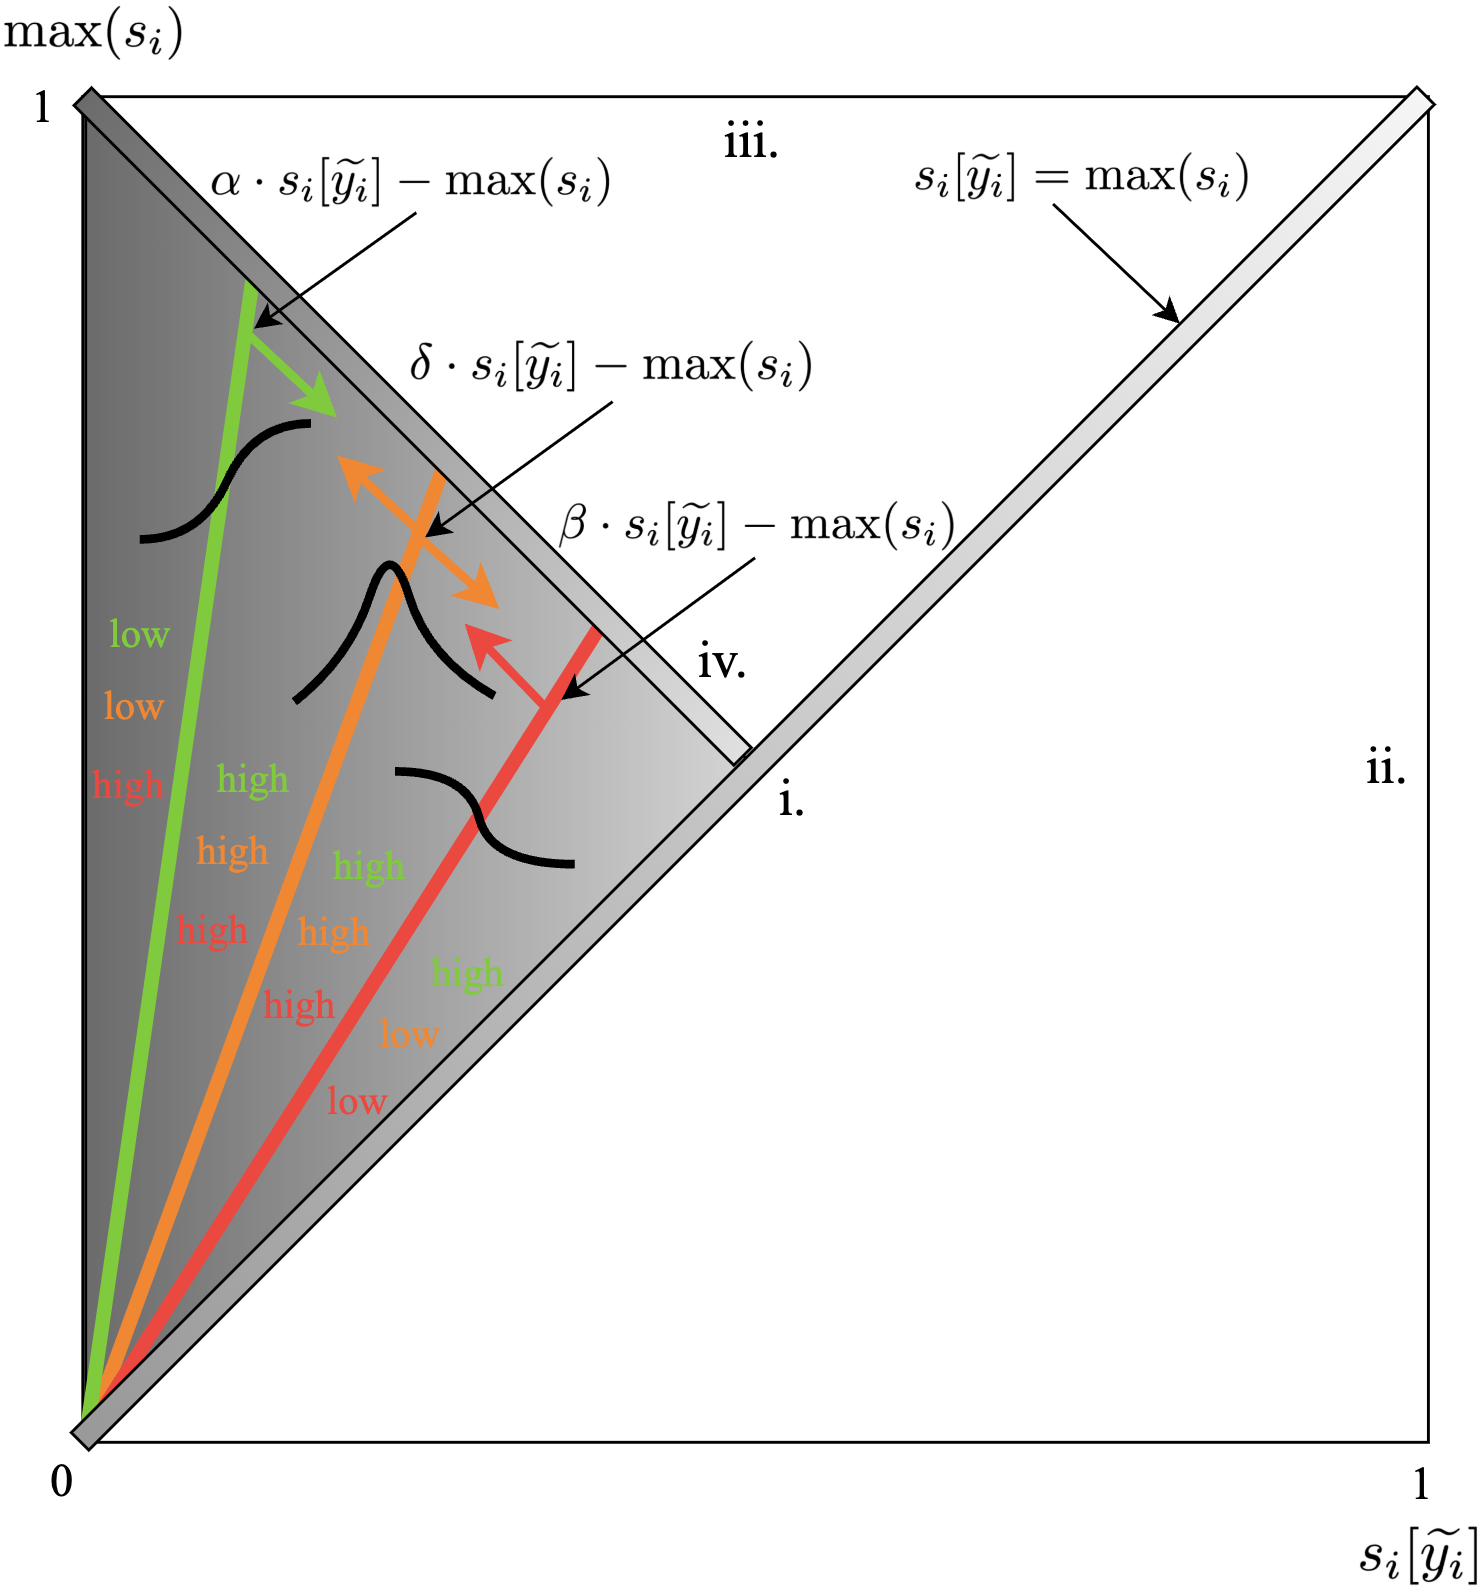
\includegraphics[scale=0.25]{graph.png}
    \caption{A graphical representation of the LiLAW weighting method. Darker areas correspond to high loss regions (due to disagreement and/or unconfidence) and lighter areas correspond to low loss regions (due to agreement and/or confidence). The three weight functions in Equations (2), (3), and (4) correspond to the green, red, and orange lines, respectively, with the colored arrows representing the direction of descent for each corresponding weight function. Note also that Equations (2) and (3) use a sigmoid and Equation (4) uses a radial basis function. We also signify whether each weight is high or low in a given region.}
    \vspace{-1em}
    \label{fig:graph}
\end{figure}
\vspace{-1em}
The above constraints form a region, shown in gray in Figure \ref{fig:graph}, which contains the values that $s_i[\widetilde{y_i}]$ and $\max(s_i)$ can attain. The darker shading corresponds high loss areas and the lighter shading corresponds to lower loss. The diagonal band going from the bottom left to the top right corresponds to when $s_i[\widetilde{y_i}] = \max(s_i)$. Closer to the bottom left, we make unconfident predictions and closer to the top right, we make more confident predictions. The remaining shaded areas correspond to when $s_i[\widetilde{y_i}] < \max(s_i)$. Near the top left of the region, we have more confident predictions and near the bottom left, we have more unconfident predictions. Closer to the center of the region, we have somewhat unconfident predictions. Our method attempts to push unconfident  predictions to being confident and incorrect predictions to being correct (with regards to the observed label). %As a result, it is able to deal with label noise. 

The above properties provide granularity to help us identify predictions as being incorrect or correct (with respect to the observed label) and unconfident or confident. However, they are not sufficient to learn to adaptively weight the losses of certain samples throughout the course of training. Therefore, we use parameters to control the relationship between $s_i[\widetilde{y_i}]$ and $\max(s_i)$ during training. We define three scalar parameters, $\alpha, \beta, \delta$ to define the contribution of different data points to the loss function.

We define our unweighted loss function as follows (in our case, $\mathcal{L}$ is cross-entropy loss or focal loss~\citep{focalloss}): 
\begin{align}
    \mathcal{L} = \ell(f_{\theta}(x_i), \widetilde{y_i})
\end{align}

We define the weights pertaining to $\alpha,\beta,\delta$ as follows:
\begin{align}
    \mathcal{W}_\alpha (s_i, \widetilde{y_i}) = \sigma(\alpha \cdot s_i[\widetilde{y_i}] - \max(s_i))
\end{align}
\begin{align}
    \mathcal{W}_\beta (s_i, \widetilde{y_i}) = \sigma(-(\beta \cdot s_i[\widetilde{y_i}] - \max(s_i)))
\end{align}
\begin{align}
    \mathcal{W}_\delta (s_i, \widetilde{y_i}) = \exp\biggl(-\frac{(\delta \cdot s_i[\widetilde{y_i}] - \max(s_i))^2}{2}\biggr)
\end{align}

\noindent We calculated the weight for each sample as follows:
\begin{align}
    \mathcal{W}(s_i, \widetilde{y_i}) = \mathcal{W}_\alpha (s_i, \widetilde{y_i}) + \mathcal{W}_\beta (s_i, \widetilde{y_i}) + \mathcal{W}_\delta (s_i, \widetilde{y_i})
\end{align}

\noindent and define our LiLAW (weighted) loss function as follows:
\begin{align}
\mathcal{L}_{W} &= \mathcal{W}(s_i, \widetilde{y_i}) \cdot \mathcal{L}
\end{align}

We define a sample's weight as the sum of $\mathcal{W}_\alpha$, $\mathcal{W}_\beta$, and $\mathcal{W}_\delta$ so that the final contribution of a sample is not governed by one parameter, but by the combined effect of all three. Easy, moderate, and hard samples primarily activate $\mathcal{W}_\alpha$, $\mathcal{W}_\beta$, and $\mathcal{W}_\delta$, respectively, while their overlap provides smooth transitions near boundaries and keeps LiLAW differentiable with respect to $\alpha,\beta,\delta$. Geometrically, $\mathcal{W}_\alpha$ is high when $\alpha$ is large and/or $s_i[\widetilde{y_i}] \ll \max(s_i)$, $\mathcal{W}_\beta$ when $\beta$ is small and/or $s_i[\widetilde{y_i}] \approx \max(s_i)$, and $\mathcal{W}_\delta$ when $\delta$ is large and/or $s_i[\widetilde{y_i}]$ is moderately close to $\max(s_i)$. We initialize $\alpha \leq \delta \leq \beta$, enforce $\alpha \geq 1$ to weight unconfident samples sufficiently, and require $\delta \geq \beta$ so that moderate samples receive more weight than easy ones but less than hard ones.

Now, let's consider $\mathcal{W}_\alpha = \sigma(\alpha \cdot s_i[\widetilde{y_i}] - \max(s_i))$.

\noindent$\mathcal{W}_\alpha < 0.5$ when:
\begin{align}
    \alpha \cdot s_i[\widetilde{y_i}] - \max(s_i) &< 0 \\
    %\alpha \cdot s_i[\widetilde{y_i}] &< \max(s_i) \\
     \implies\alpha \cdot s_i[\widetilde{y_i}] < \max(s_i) &\leq 1 \text{ by (ii)}
\end{align}
$\mathcal{W}_\alpha \geq 0.5$ when:
\begin{align}
    \alpha \cdot s_i[\widetilde{y_i}] - \max(s_i) &\geq 0 \\
    %\alpha \cdot s_i[\widetilde{y_i}] &\geq \max(s_i) \\
    \implies \alpha \cdot s_i[\widetilde{y_i}] \geq \max(s_i) &\geq s_i[\widetilde{y_i}] \text{ by (i)}
\end{align}
As such, the upper and lower bounds on $\mathcal{W}_\alpha$, as seen in Figure~\ref{fig:graph}, are as follows:
\vspace{-0.5em}
\begin{align}
    -1 \leq \alpha \cdot s_i[\widetilde{y_i}] - \max(s_i) &\leq \alpha-1 \\
    \implies 0.2689 \approx \sigma(-1) \leq \mathcal{W}_\alpha &\leq \sigma(\alpha-1) < 1
\end{align}
Now, let's consider $\mathcal{W}_\beta = \sigma(-(\beta \cdot s_i[\widetilde{y_i}] - \max(s_i)))$. 

\noindent$\mathcal{W}_\beta < 0.5$ when:
\vspace{-0.5em}
\begin{align}
    \beta \cdot s_i[\widetilde{y_i}] - \max(s_i) &> 0 \\
    \implies \beta \cdot s_i[\widetilde{y_i}] > \max(s_i) &\geq s_i[\widetilde{y_i}] \text{ by (i)}
    %\beta \cdot s_i[\widetilde{y_i}] &> \max(s_i) \\
    \vspace{-0.5em}
\end{align}
$\mathcal{W}_\beta \geq 0.5$ when:
\vspace{-0.5em}
\begin{align}
    \beta \cdot s_i[\widetilde{y_i}] - \max(s_i) &\leq 0 \\ 
    %\beta \cdot s_i[\widetilde{y_i}] &\leq \max(s_i) \\
    \implies \beta \cdot s_i[\widetilde{y_i}] \leq \max(s_i) &\leq s_i[\widetilde{y_i}] \text{ by (ii)}
    \vspace{-0.5em}
\end{align}
The upper and lower bounds on $\mathcal{W}_\beta$, as seen in Figure~\ref{fig:graph}, are as follows:
\vspace{-0.5em}
\begin{align}
    1-\beta \leq \beta \cdot s_i[\widetilde{y_i}] - \max(s_i) &\leq 1 \\
    \implies 0 < \sigma(1-\beta) \leq \mathcal{W}_\beta &\leq \sigma(1) \approx 0.7311
    \vspace{-0.5em}
\end{align}
Finally, consider $\mathcal{W}_\delta (s_i, \widetilde{y_i}) = \exp\bigl(-\frac{(\delta \cdot s_i[\widetilde{y_i}] - \max(s_i))^2}{2}\bigr)$. $\mathcal{W}_\delta = 1$ when:
\vspace{-0.5em}
\begin{align}
    \delta \cdot s_i[\widetilde{y_i}] - \max(s_i) = 0 \implies
    \delta \cdot s_i[\widetilde{y_i}] = \max(s_i)
\end{align}
Otherwise, $0 < \mathcal{W}_\delta < 1$, with $\mathcal{W}_\delta$ tending towards zero as $\delta \cdot s_i[\widetilde{y_i}]$ and $\max(s_i)$ grow apart.


\begin{algorithm}[h]
\caption{Training with LiLAW}
\begin{algorithmic}[1]
        \STATE \textbf{Inputs:} training set $(\mathcal{D}_{t})$, validation set $(\mathcal{D}_{v})$, classifier model $f_\theta$, LiLAW parameters $\alpha, \beta, \delta$, optimizer for $\alpha, \beta, \delta, \theta$, learning rates $\alpha_{lr}, \beta_{lr}, \delta_{lr},$ weight decay values $\alpha_{wd}, \beta_{wd}, \delta_{wd}$
        \STATE \textbf{Output:} classifier model trained using LiLAW
            \FOR{epoch $\gets 1$ \textbf{to} $n$}
                \FOR{batch $(x_t, \widetilde{y}_t) \gets $ dataloader($\mathcal{D}_{t}$)}
                    \STATE set requires\_grad to False on $\alpha, \beta, \delta,$ True on $\theta$
                    \STATE $s = \mathrm{softmax}(f_\theta(x_t))$
                    \STATE calculate train loss $\mathcal{L}_{W} = \mathcal{W}(s, \widetilde{y}_t) \cdot \ell(f_{\theta}(x_t), \widetilde{y}_t)$
                    \STATE $\mathcal{L}_{W}$.backward()
                    \STATE optimizer.step() to update $\theta$
                    \STATE optimizer.zero\_grad()
                    \STATE choose a random batch $(x_v, \widetilde{y}_v)$ $\gets$ dataloader($\mathcal{D}_{v}$)
                    \STATE set requires\_grad to True on $\alpha, \beta, \delta$, False on $\theta$
                    \STATE $s = \mathrm{softmax}(f_\theta(x_v))$
                    \STATE calculate val loss $\mathcal{L}_{W} = \mathcal{W}(s, \widetilde{y}_v) \cdot \ell(f_{\theta}(x_v), \widetilde{y}_v)$
                    \STATE $\mathcal{L}_{W}$.backward()
                    \STATE $\alpha = \alpha - \alpha_{lr} * (\nabla_{\alpha}\mathcal{L}_{W} + \alpha_{wd} * \alpha)$
                    \STATE $\beta = \beta - \beta_{lr} * (\nabla_{\beta}\mathcal{L}_{W} + \beta_{wd} * \beta)$
                    \STATE $\delta = \delta - \delta_{lr} * (\nabla_{\delta}\mathcal{L}_{W} + \delta_{wd} * \delta)$
                    \STATE $\nabla_{\alpha}\mathcal{L}_{W} = \nabla_{\beta}\mathcal{L}_{W} = \nabla_{\delta}\mathcal{L}_{W} = 0$
                \ENDFOR
            \ENDFOR
            \STATE \textbf{return} $f_\theta(x)$
\end{algorithmic}
\label{algo}
\end{algorithm}

During training (see Algorithm~\ref{algo}), we aim to find the model parameters $\theta^*$ that best minimize LiLAW loss on the training set using the three parameters $\alpha^*, \beta^*, \delta^*$ that best minimize LiLAW loss on the validation set to get the objective:
\vspace{-0.5em}
\begin{align}
    \displaystyle\theta^* = \arg\min_{\theta} \sum_{(x_i, \widetilde{y_i}) \in \mathcal{D}_{t}}\mathcal{L}_{W_{\alpha^*, \beta^*, \delta^*}} \text{ such that } \\
    \alpha^*, \beta^*, \delta^* = \displaystyle\arg\min_{\alpha, \beta, \delta} \sum_{(x_i, \widetilde{y_i}) \in \mathcal{D}_{v}}\mathcal{L}_{W_{\theta^*}}
    \vspace{-2em}
\end{align}
Note that $\mathcal{L}_{W_{\alpha^*, \beta^*, \delta^*}}$ is the loss computed using parameters $\alpha^*, \beta^*, \delta^*$ and $\mathcal{L}_{W_{\theta^*}}$ is the loss computed using the network parameters $\theta^*$. This objective is similar to the formulation in~\citet{jain_improving_2024}; however, we do not require an instance-wise weighting function, but a more general weighting function based on $\alpha, \beta, \delta$. 
Similar to MOLERE~\citep{jain_improving_2024}, LRW~\citep{ren_learning_2019}, and MAML~\citep{finn_model-agnostic_2017}, we perform stochastic gradient updates on validation mini-batches to update the three parameters $\alpha, \beta, \delta$.

We generally see that:
\vspace{-1em}
\begin{enumerate}[leftmargin=*,labelindent=0pt,label=\textbf{--}]
    \itemsep-0.2em 
    \item $\mathcal{W}_\alpha$ is high when $\alpha$ is large or when $s_i[\widetilde{y_i}] = \max(s_i)$ and $\max(s_i)$ is high (agrees confidently = \textit{easy})
    \item $\mathcal{W}_\beta$ is high when $\beta$ is small or when $s_i[\widetilde{y_i}] < \max(s_i)$ and $\max(s_i)$ is high (disagrees confidently = \textit{hard})
    \item $\mathcal{W}_\delta$ is high when $\delta$ is large or when $\max(s_i)$ is low \\(agrees or disagrees unconfidently = \textit{moderate})
\end{enumerate}

Prior meta-reweighting work~\citep{ren_learning_2019} assumes a small clean validation set to steer training towards the clean-label objective. Our setting is different and more realistic: we explicitly allow the meta-validation set to contain label noise, because a clean set is often unavailable in practice. Using a noisy training set and a noisy validation set, as in LiLAW, is well‑motivated, as demonstrated by the theoretical and empirical results of~\citet{chen_robustness}. Specifically, they show that during training, maximizing accuracy over a sufficiently large noisy dataset leads to an approximately optimal classifier. For validation, they show that using a noisy validation set is reasonable because the accuracy on held‑out noisy samples is as an unbiased estimator of the accuracy under the noisy data distribution. We also extend the results from~\citet{gui2021towards}'s work to prove that diagonally dominant noise is sufficient for LiLAW to separate clean and noisy labels in~\ref{proof:diag}.

\section{Experiments}
\label{sec:experiments}

We conducted extensive experiments with and without LiLAW to comprehensively assess its ability to boost test performance. We used H-CAT~\citep{seedat_dissecting_2024}, an API interface for several hardness and data characterization techniques, to study LiLAW. We emphasize that our goal is not to achieve state-of-the-art results, but to demonstrate the effectiveness of LiLAW in various settings. % To this end, we make the following considerations detailed below.

We show how the weight functions (2), (3), and (4) change with respect to $\alpha, \beta, \delta$ in~\ref{supp:derivative}. We also show that training with and without LiLAW share the same time complexity in~\ref{supp:timecomplexity} and space complexity in~\ref{supp:spacecomplexity}. We also extend LiLAW to be used for multi-label classification in~\ref{sec:multilabel} and regression in~\ref{sec:regression}. We compare the three formulations in~\ref{comparison}.

\subsection{Datasets}
\label{sec:datasets}

We use the CIFAR-100 dataset~\citep{cifar100} (and CIFAR-10~\citep{cifar10}, FashionMNIST~\citep{fashionmnist}, MNIST~\cite{deng2012mnist}), but we do not use the full training sets. Instead, we reserve a portion of the training set to serve as the validation set to evaluate and adjust our model's performance, as required by our method. We call our modified datasets, CIFAR-100-M, CIFAR-10-M, FashionMNIST-M, and MNIST-M, respectively. To demonstrate generalizability and applicability to the medical domain, we evaluate LiLAW on ten 2D datasets with different medical imaging modalities focusing on multi-class classification tasks from MedMNISTv2~\citep{medmnistv1,medmnistv2,doerrich2024rethinking} at varying noise levels. 

%We also demonstrate strong results on a non-imaging dataset, ECG5000, which contains time-series data for heartbeat classification with 5 highly imbalanced classes.

To demonstrate LiLAW's effectivness when augmenting real data with synthetic data, we use real datasets (UNBC-McMaster~\citep{lucey2011painful} and UofR~\citep{rezaei2020unobtrusive}) and a synthetic dataset (\synpain~\citep{taati2025synpain}) for pain detection. UofR comprises of images from people with dementia (Dementia) and without dementia (Healthy). \synpain also contains a subset of images, \synpain-Old, which contain samples from adults of age 75+. For gait classification, we use a real dataset (PD-GaM~\citep{adeli2025gaitgen}) and a synthetic dataset (\gaitgen~\citep{adeli2025gaitgen}). We then use the ECG5000~\citep{physiobank2000physionet} dataset with simple augmentations (say ECG5000-A) containing time-series data for heartbeat classification. We show that LiLAW improves performance and generally improves fairness across sex, race, and age with the Adult dataset~\citep{adult} for income prediction. %See~\ref{fairness} for results.

\subsection{Models}
\label{sec:models}
We use models with a varying number of parameters to demonstrate the utility of LiLAW: ViT-Base-16-224~\citep{vit} for the general imaging datasets (CIFAR-100-M, CIFAR-10-M, FashionMNIST-M, MNIST-M), ResNet-18~\citep{resnet} for the medical imaging datasets (ten 2D MedMNISTv2 datasets), the Pairwise with Contrastive Training (PwCT) model~\cite{rezaei2020unobtrusive} for the pain detection datasets, the MotionClassifier model~\cite{adeli2025gaitgen} for the gait classification datasets, a simple Stacked LSTM model for the ECG5000-A dataset, and a simple 3-layer MLP for the Adult census dataset. Further implementation details are in~\ref{imp}.

\subsection{Evaluation}

We study the effectiveness of LiLAW extensively with various levels of injected noise with symmetric and asymmetric noise (see Table \ref{table:noisetypes}) and with ten MedMNISTv2 datasets (see Table \ref{table:medmnist} and Figure \ref{fig:med1}). In the Appendix, we evaluate LiLAW's performance with ablations on $\alpha,\beta,\delta$ (see~\ref{supp:ablation}, Table \ref{table:ablation}) to show that including all three parameters achieves the best results, report the results at different noise levels (see~\ref{supp:noiselevel}, Table \ref{table:noiselevels}) to show the effectiveness of LiLAW even in high-noise scenarios, evaluate with and without calibration (using temperature scaling) (see~\ref{supp:calibration}, Table \ref{table:calibration}), with and without a clean validation set (see~\ref{supp:cleanvalset}, Table \ref{table:cleanval}) to show that LiLAW does not need a clean validation set and outperforms noise pruning, and with various random seeds (see~\ref{supp:randseed}, Table \ref{table:seeds}) to show that using LiLAW results in a consistent improvements.  We show that LiLAW is effective with two different loss functions (see~\ref{supp:loss}, Table \ref{table:losses}), with different validation set sizes (see~\ref{supp:valsize}, Table \ref{table:valsize}), and with and without the same validation and training distribution (see~\ref{supp:valdist}, Table \ref{table:valdist}). We report results on four general imaging datasets (see~\ref{supp:moredatasets}, Table \ref{table:datasets}) and report the accuracy (see Table \ref{table:medmnist} and Figure \ref{fig:med1}) and AUROC (see~\ref{supp:medmnist}, Table~\ref{table:medmnist2}) results for MedMNISTv2. We also provide some baselines on identifying mislabels (see~\ref{supp:comp}, Table~\ref{table:comp}), provide results on using LiLAW with synthetic datasets and augmented datasets (see~\ref{sec:pain}, Table~\ref{x} for pain detection using the regression formulation,~\ref{sec:gait}, Table~\ref{tab:gait} for gait classification, and~\ref{sec:heart}, Table~\ref{tab:ecg} for heartbeat classification), and provide fairness results on the Adult dataset along with a proof of why LiLAW helps in~\ref{fairness}.

%To comprehensively understand LiLAW's impact, we evaluated gains in test accuracy (top-1 and top-5) and AUROC with and without LiLAW across different settings. For the selected MedMNISTv2 datasets, we report the test accuracy (top-1 only, since some have $<5$ classes) and AUROC.

\subsection{Performance Comparison: General Imaging}

%In all of the following tables, the results show test performance without LiLAW along with the difference in performance, i.e. the improvement (\textcolor{Green}{$\uparrow$}) or deterioration (\textcolor{BrickRed}{$\downarrow$}) with LiLAW, respectively. 

\iffalse
\begin{figure}[htb!]
    \centering
    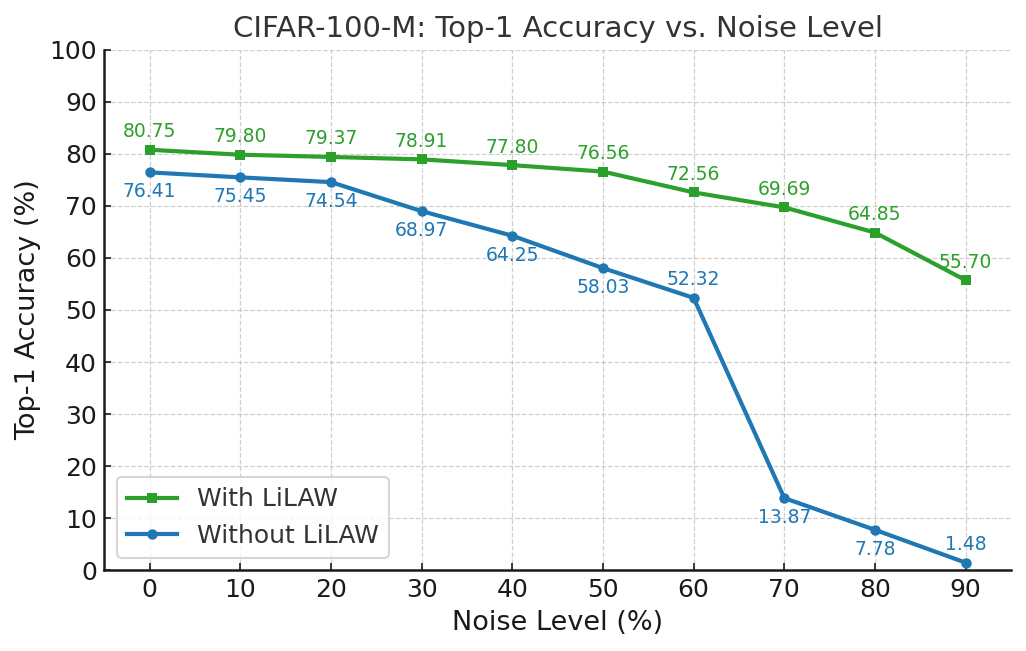
\includegraphics[scale=0.34]{ciftop1.png}
    \caption{Top-1 accuracy with LiLAW with linear probing on the last two layers, without LiLAW with linear probing on the last two layers, and without LiLAW with fine-tuning on the full network using different levels of symmetric noise on CIFAR-100-M.} % with a random seed of 42.}
    \label{fig:noiselevel}
\end{figure}
\fi

For Tables~\ref{table:noisetypes}, \ref{table:noiselevels}-\ref{table:cleanval}, and \ref{table:losses}-\ref{table:datasets}, for the metrics in each column, we report performance with full fine-tuning without LiLAW and the improvement(\textcolor{Green}{$\uparrow$})/deterioration(\textcolor{BrickRed}{$\downarrow$}) with linear probing (last 2 layers) without LiLAW and the additional improvement(\textcolor{Green}{$\uparrow$})/deterioration(\textcolor{BrickRed}{$\downarrow$}) with linear probing with LiLAW. For the other tables, we either train a model from scratch or use full fine-tuning to report results without LiLAW and the improvement(\textcolor{Green}{$\uparrow$})/deterioration(\textcolor{BrickRed}{$\downarrow$}) with LiLAW.

\begin{table}[h!] \centering \resizebox{\columnwidth}{!}{\begin{tabular}{lccc} \hline \textbf{Noise Type} & \textbf{Top-1 Acc. (\%)} & \textbf{Top-5 Acc. (\%)} & \textbf{AUROC} \\ \hline Symmetric & 58.03 \textcolor{Green}{$\uparrow$} 17.17 \textcolor{Green}{$\uparrow$} 1.35 & \hspace{0.5em}85.42 \textcolor{Green}{$\uparrow$} \hspace{0.5em}7.19 \textcolor{Green}{$\uparrow$} 0.67\hspace{0.5em} & 0.9706 \textcolor{Green}{$\uparrow$} 0.0105 \textcolor{Green}{$\uparrow$} 0.0013 \\ Asymmetric & 34.37 \textcolor{Green}{$\uparrow$} 40.32 \textcolor{Green}{$\uparrow$} 1.44 & 65.75 \textcolor{Green}{$\uparrow$} 26.51 \textcolor{Green}{$\uparrow$} 0.82 & 0.9255 \textcolor{Green}{$\uparrow$} 0.0537 \textcolor{Green}{$\uparrow$} 0.0017 \\ \hline \end{tabular}} \caption{CIFAR-100-M on different noise types at 50\% noise level. \label{table:noisetypes}} \end{table}
\vspace{-1em}
In~\ref{supp:noiselevel}, Table~\ref{table:noiselevels}, we consider the test results at various noise levels from 0\% to 90\%. At each noise level, LiLAW yields higher test accuracy and AUROC compared to without it. %Note that with LiLAW, we recover noiseless top-1 accuracy when training with up to 50\% noise. 
In Table \ref{table:noisetypes}, for both symmetric and asymmetric noise, we see that LiLAW enhances performance. Also, models do not overfit as quickly with LiLAW across all noise levels and noise types. Under noisy settings, how a pretrained model is used while fine-tuning has a large effect on the performance. As mentioned in~\citet{marrium2024implicit}, full fine-tuning adapts all parameters of a pre-trained model to a downstream task with high time and space complexity while also severely overfitting to noise. On the other hand, linear probing (in our case, on the last two layers), only a few parameters are tuned to the downstream task and the risk of overfitting is drastically reduced. In addition to linear probing, we use LiLAW to further improve results.

\subsection{Performance Comparison: Medical Imaging}

\begin{table*}[h]
\centering
\footnotesize{
\centering
{
\begin{tabular}{l|cccccc}
\hline
 & & & \textbf{Acc. (\%)} & & & \\
\hline
\textbf{Dataset} & \textbf{0\% Noise} & \textbf{10\% Noise} & \textbf{20\% Noise} & \textbf{30\% Noise} & \textbf{40\% Noise} & \textbf{50\% Noise} \\
\hline
PathMNIST & 95.49 \textcolor{Green}{$\uparrow$} 0.08 & 95.38 \textcolor{BrickRed}{$\downarrow$} 0.08 & 94.70 \textcolor{Green}{$\uparrow$} 0.20 & 94.19 \textcolor{BrickRed}{$\downarrow$} 0.59 & 94.01 \textcolor{Green}{$\uparrow$} 0.18 & 92.87 \textcolor{Green}{$\uparrow$} 0.69 \\
\hline
DermaMNIST & 79.88 \textcolor{Green}{$\uparrow$} 0.88 & 76.12 \textcolor{Green}{$\uparrow$} 1.80 & 74.38 \textcolor{Green}{$\uparrow$} 2.13 & 73.92 \textcolor{Green}{$\uparrow$} 0.27 & 71.89 \textcolor{Green}{$\uparrow$} 1.46 & 68.03 \textcolor{Green}{$\uparrow$} 4.52 \\
\hline
OCTMNIST & 75.73 \textcolor{Green}{$\uparrow$} 0.65 & 72.84 \textcolor{Green}{$\uparrow$} 4.74 & 71.42 \textcolor{Green}{$\uparrow$} 1.97 & 67.11 \textcolor{Green}{$\uparrow$} 3.44 & 68.19 \textcolor{Green}{$\uparrow$} 4.94 & 60.79 \textcolor{Green}{$\uparrow$} 7.07 \\
\hline
PneumoniaMNIST & 89.04 \textcolor{Green}{$\uparrow$} 2.61 & 85.40 \textcolor{Green}{$\uparrow$} 1.10 & 86.65 \textcolor{BrickRed}{$\downarrow$} 0.41 & 85.40 \textcolor{Green}{$\uparrow$} 4.18 & 81.50 \textcolor{Green}{$\uparrow$} 2.90 & 84.24 \textcolor{Green}{$\uparrow$} 2.14 \\
\hline
BreastMNIST & 85.83 \textcolor{Green}{$\uparrow$} 1.39 & 83.87 \textcolor{BrickRed}{$\downarrow$} 1.17 & 79.13 \textcolor{Green}{$\uparrow$} 2.96 & 78.74 \textcolor{Green}{$\uparrow$} 0.39 & 74.78 \textcolor{Green}{$\uparrow$} 6.75 & 70.10 \textcolor{Green}{$\uparrow$} 4.34 \\
\hline
BloodMNIST & 98.50 \textcolor{Green}{$\uparrow$} 0.16 & 97.24 \textcolor{Green}{$\uparrow$} 0.18 & 97.36 \textcolor{Green}{$\uparrow$} 0.21 & 96.93 \textcolor{BrickRed}{$\downarrow$} 0.28 & 95.72 \textcolor{Green}{$\uparrow$} 0.71 & 94.72 \textcolor{Green}{$\uparrow$} 0.42 \\
\hline
TissueMNIST & 68.74 \textcolor{BrickRed}{$\downarrow$} 1.33 & 65.02 \textcolor{Green}{$\uparrow$} 0.85 & 61.33 \textcolor{Green}{$\uparrow$} 1.17 & \hspace{0.5em}45.08 \textcolor{Green}{$\uparrow$} 19.16 & \hspace{0.5em}38.50 \textcolor{Green}{$\uparrow$} 13.22 & \hspace{0.5em}31.82 \textcolor{Green}{$\uparrow$} 20.41 \\
\hline
OrganAMNIST & 94.87 \textcolor{Green}{$\uparrow$} 0.18 & 94.19 \textcolor{Green}{$\uparrow$} 0.22 & 94.02 \textcolor{Green}{$\uparrow$} 0.18 & 90.76 \textcolor{Green}{$\uparrow$} 2.73 & 92.50 \textcolor{Green}{$\uparrow$} 0.52 & 89.45 \textcolor{Green}{$\uparrow$} 1.63 \\
\hline
OrganCMNIST & 90.66 \textcolor{Green}{$\uparrow$} 0.93 & 88.85 \textcolor{Green}{$\uparrow$} 1.01 & 85.37 \textcolor{Green}{$\uparrow$} 0.30 & 84.45 \textcolor{Green}{$\uparrow$} 2.73 & 84.19 \textcolor{Green}{$\uparrow$} 0.87 & 82.95 \textcolor{Green}{$\uparrow$} 1.24 \\
\hline
OrganSMNIST & 80.54 \textcolor{Green}{$\uparrow$} 0.49 & 78.28 \textcolor{Green}{$\uparrow$} 0.66 & 75.34 \textcolor{Green}{$\uparrow$} 2.16 & 72.54 \textcolor{Green}{$\uparrow$} 3.35 & 72.95 \textcolor{Green}{$\uparrow$} 1.42 & 70.82 \textcolor{Green}{$\uparrow$} 2.65 \\
\hline
\end{tabular}}} \caption{Accuracy on ten 2D datasets from MedMNISTv2 with different levels of symmetric noise. The MedMNIST experiments were done with fine-tuning on the full pretrained model without LiLAW and with LiLAW, i.e. LiLAW is effective with full model fine-tuning. \label{table:medmnist}}
\end{table*}

In Table~\ref{table:medmnist} and Figure~\ref{fig:med1}, we see the effect of LiLAW across ten 2D datasets from MedMNISTv2 with varying levels of injected symmetric label noise (see~\ref{supp:medmnist}, Table \ref{table:medmnist2}, Figure \ref{fig:med2} for AUROC metrics). Applying LiLAW across various symmetric noise levels leads to an increase in accuracy and/or AUROC in nearly all cases compared to when trained without LiLAW. When there is deterioration, it is minimal and at low noise. Given the noisiness of medical data, LiLAW's ability to enhance performance under such conditions is highly valuable, especially given that we are also performing full fine-tuning with ImageNet-21K pretraining.

\begin{figure*}[h!]
    \centering
    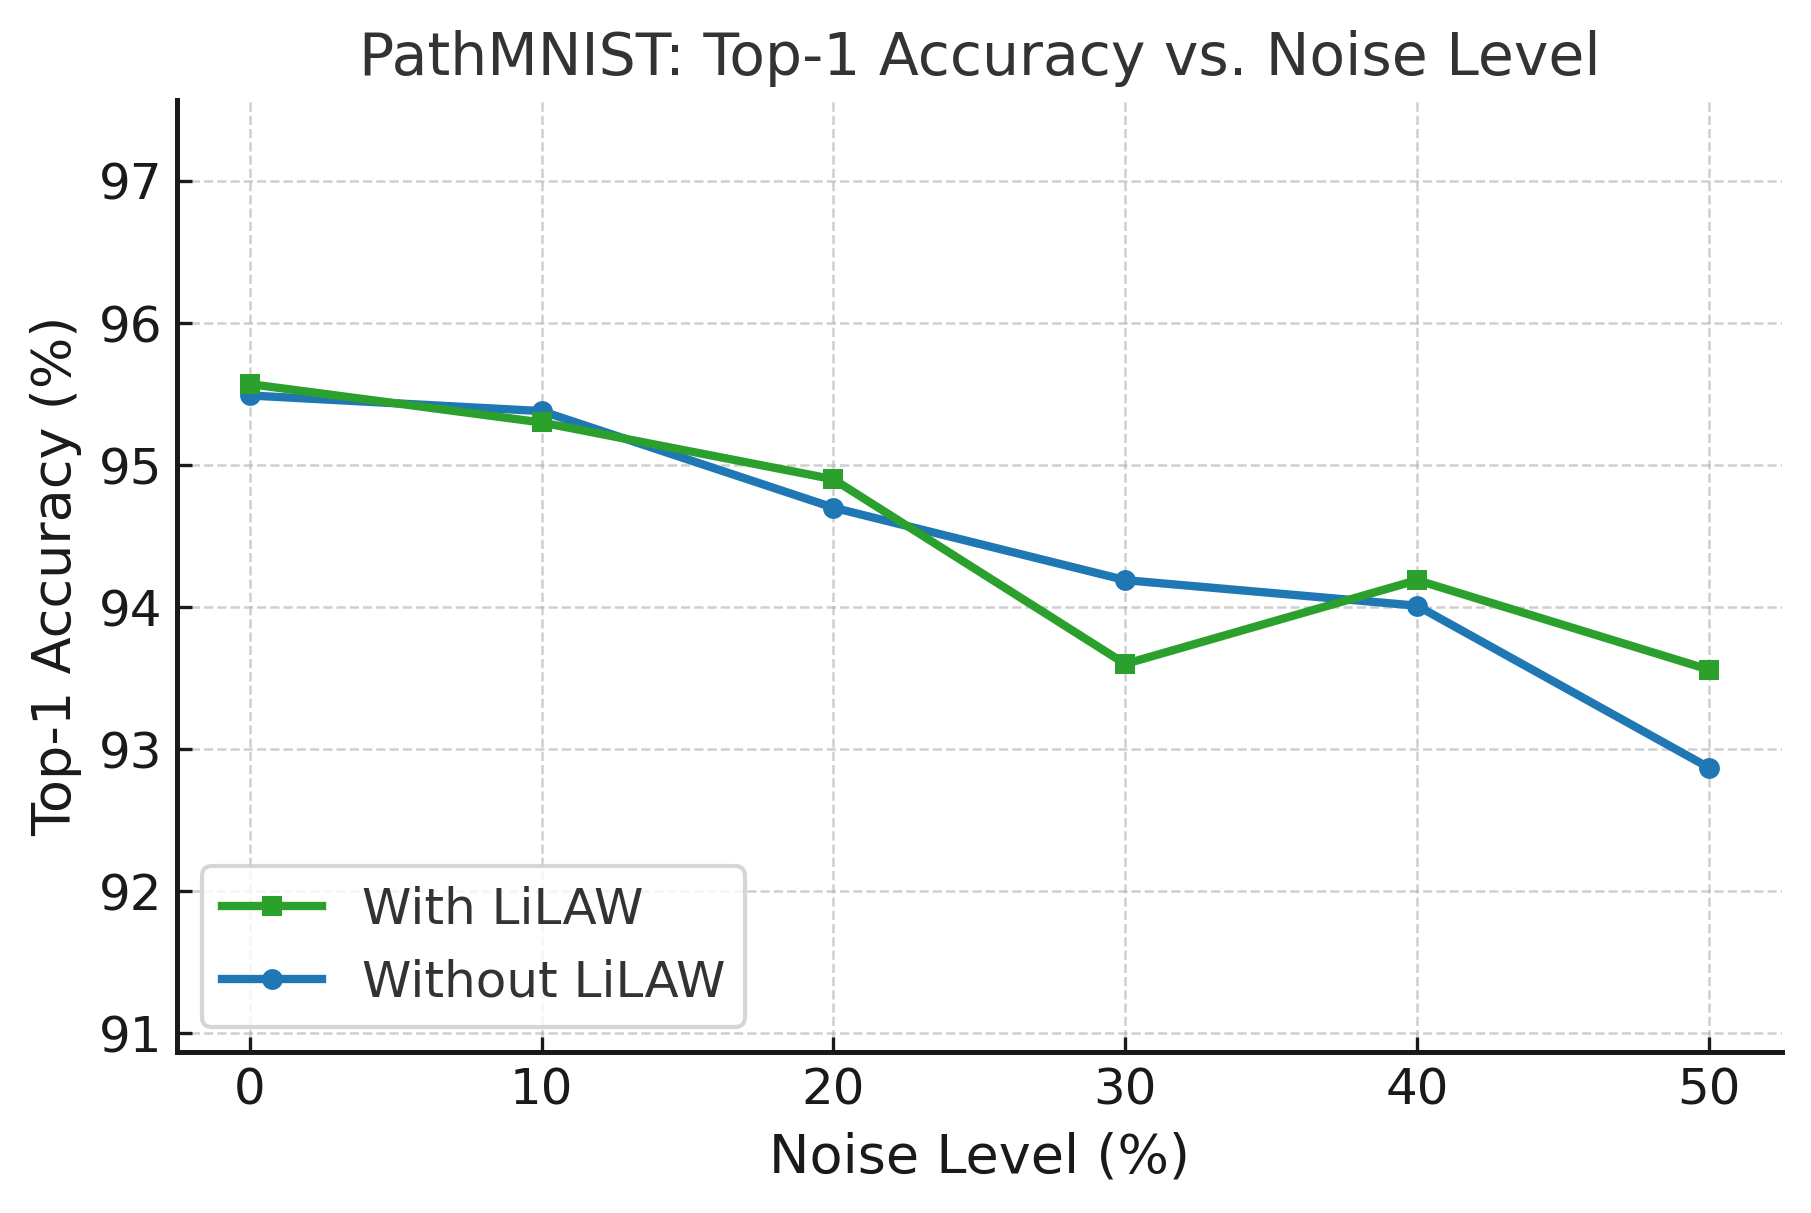
\includegraphics[scale=0.21]{path.png}
    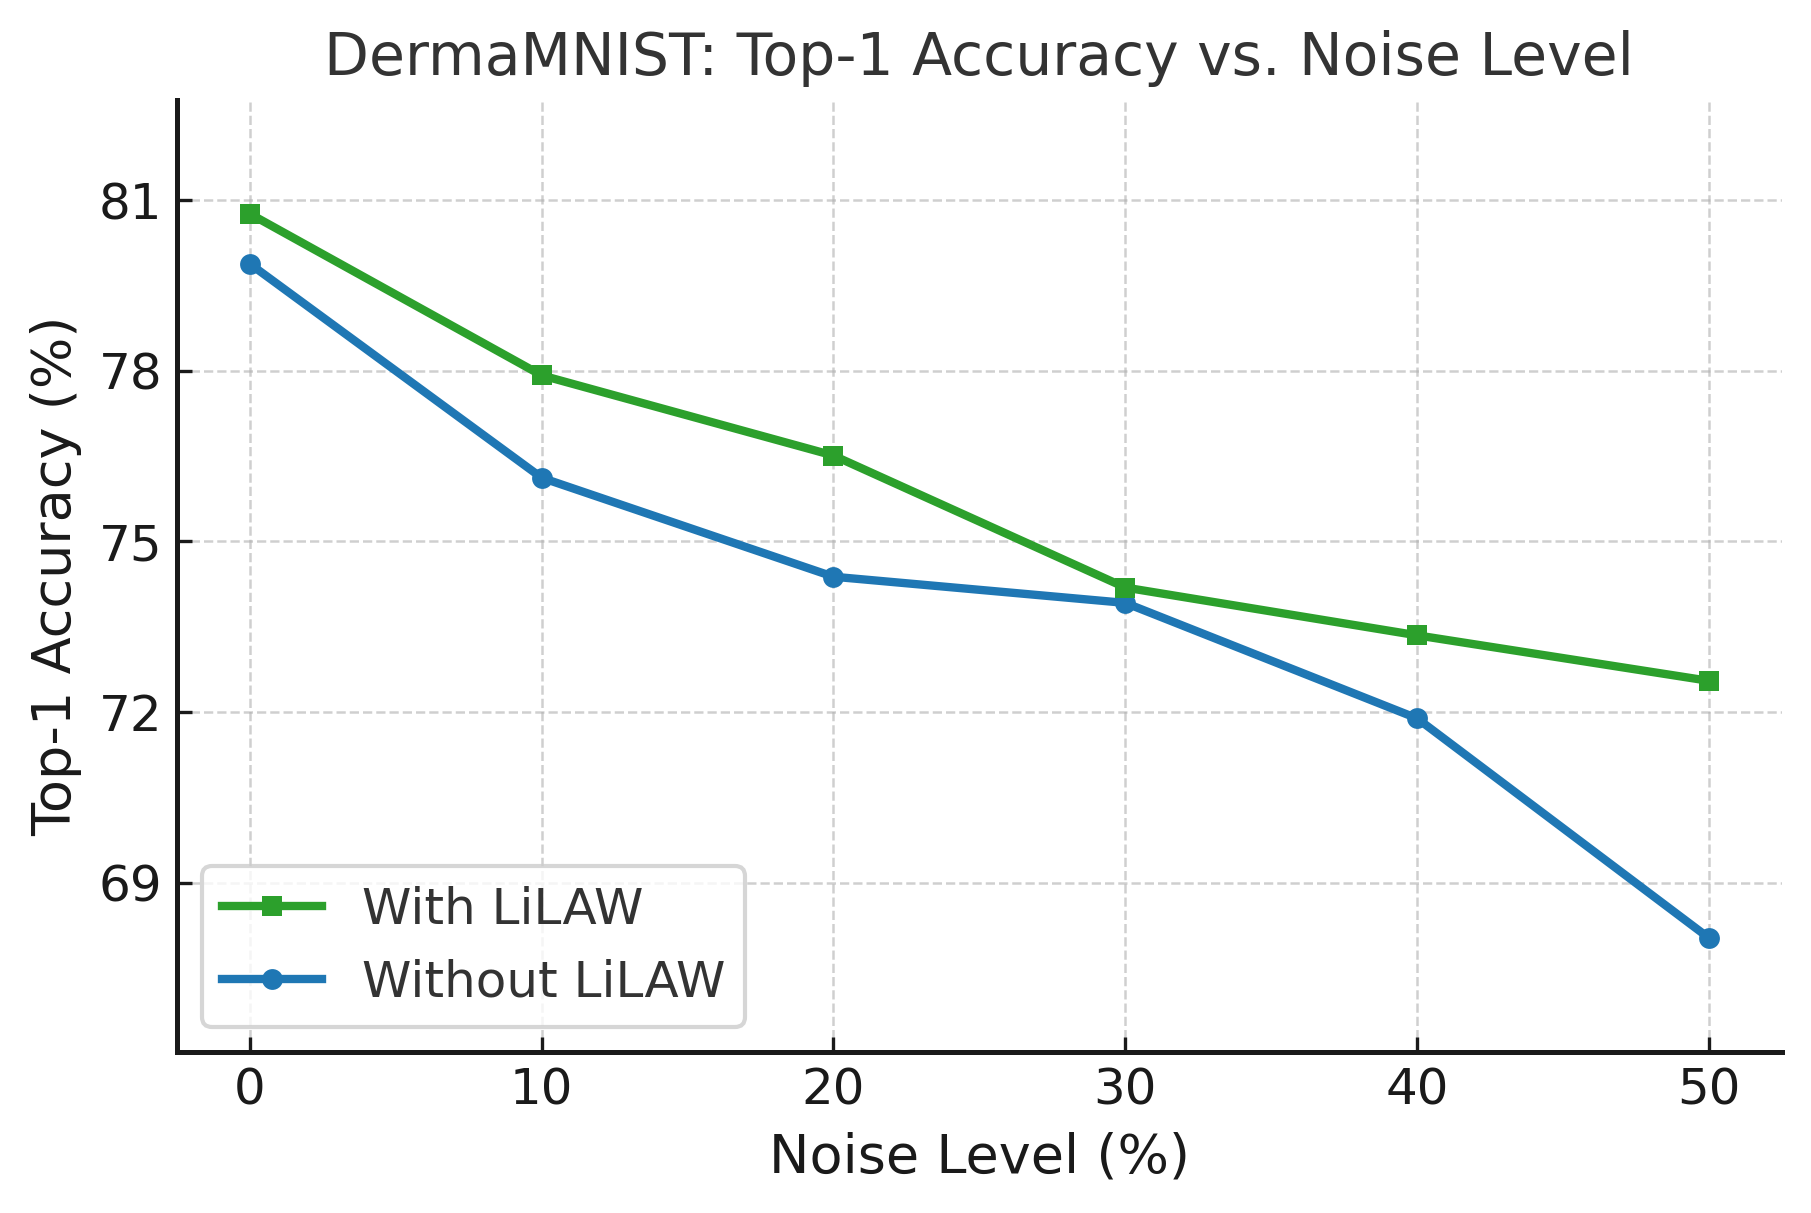
\includegraphics[scale=0.21]{derma.png}
    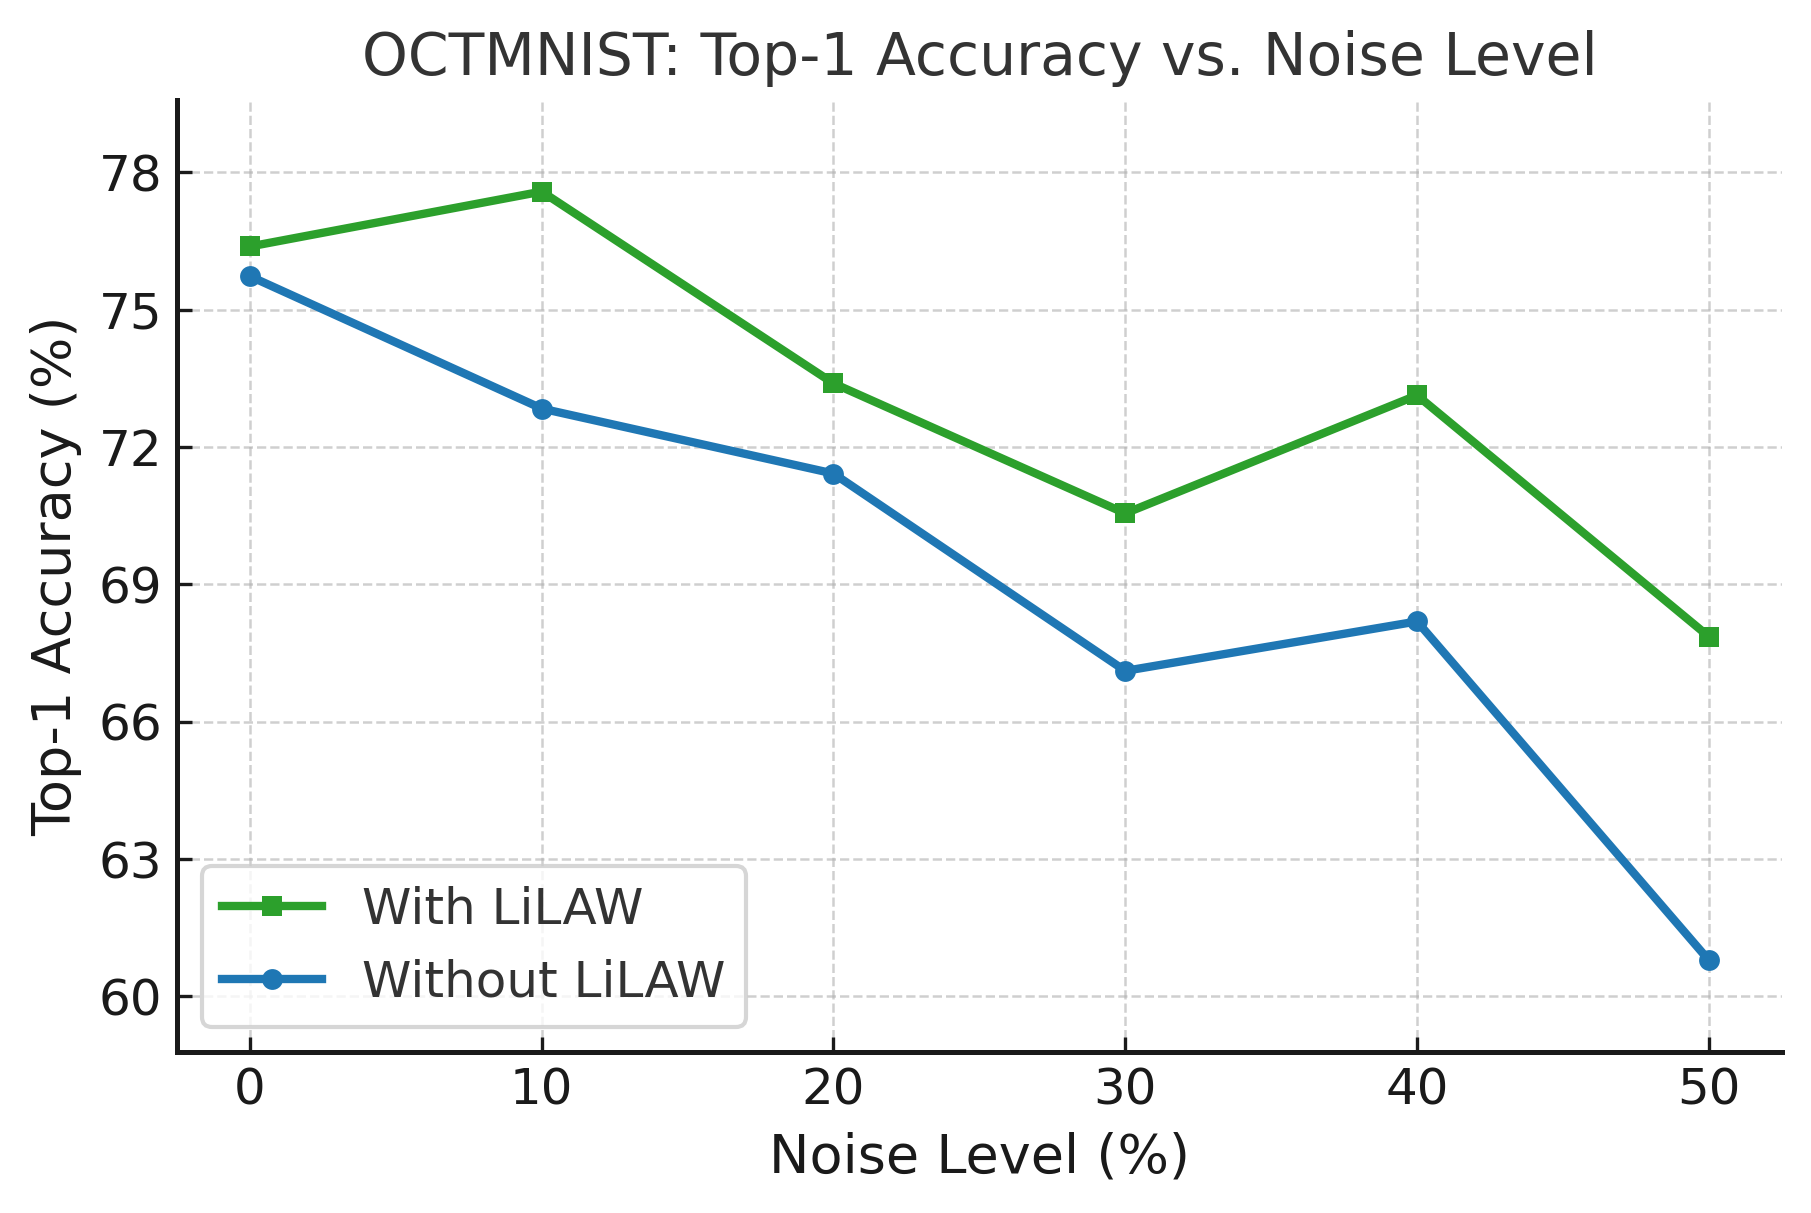
\includegraphics[scale=0.21]{oct.png}
    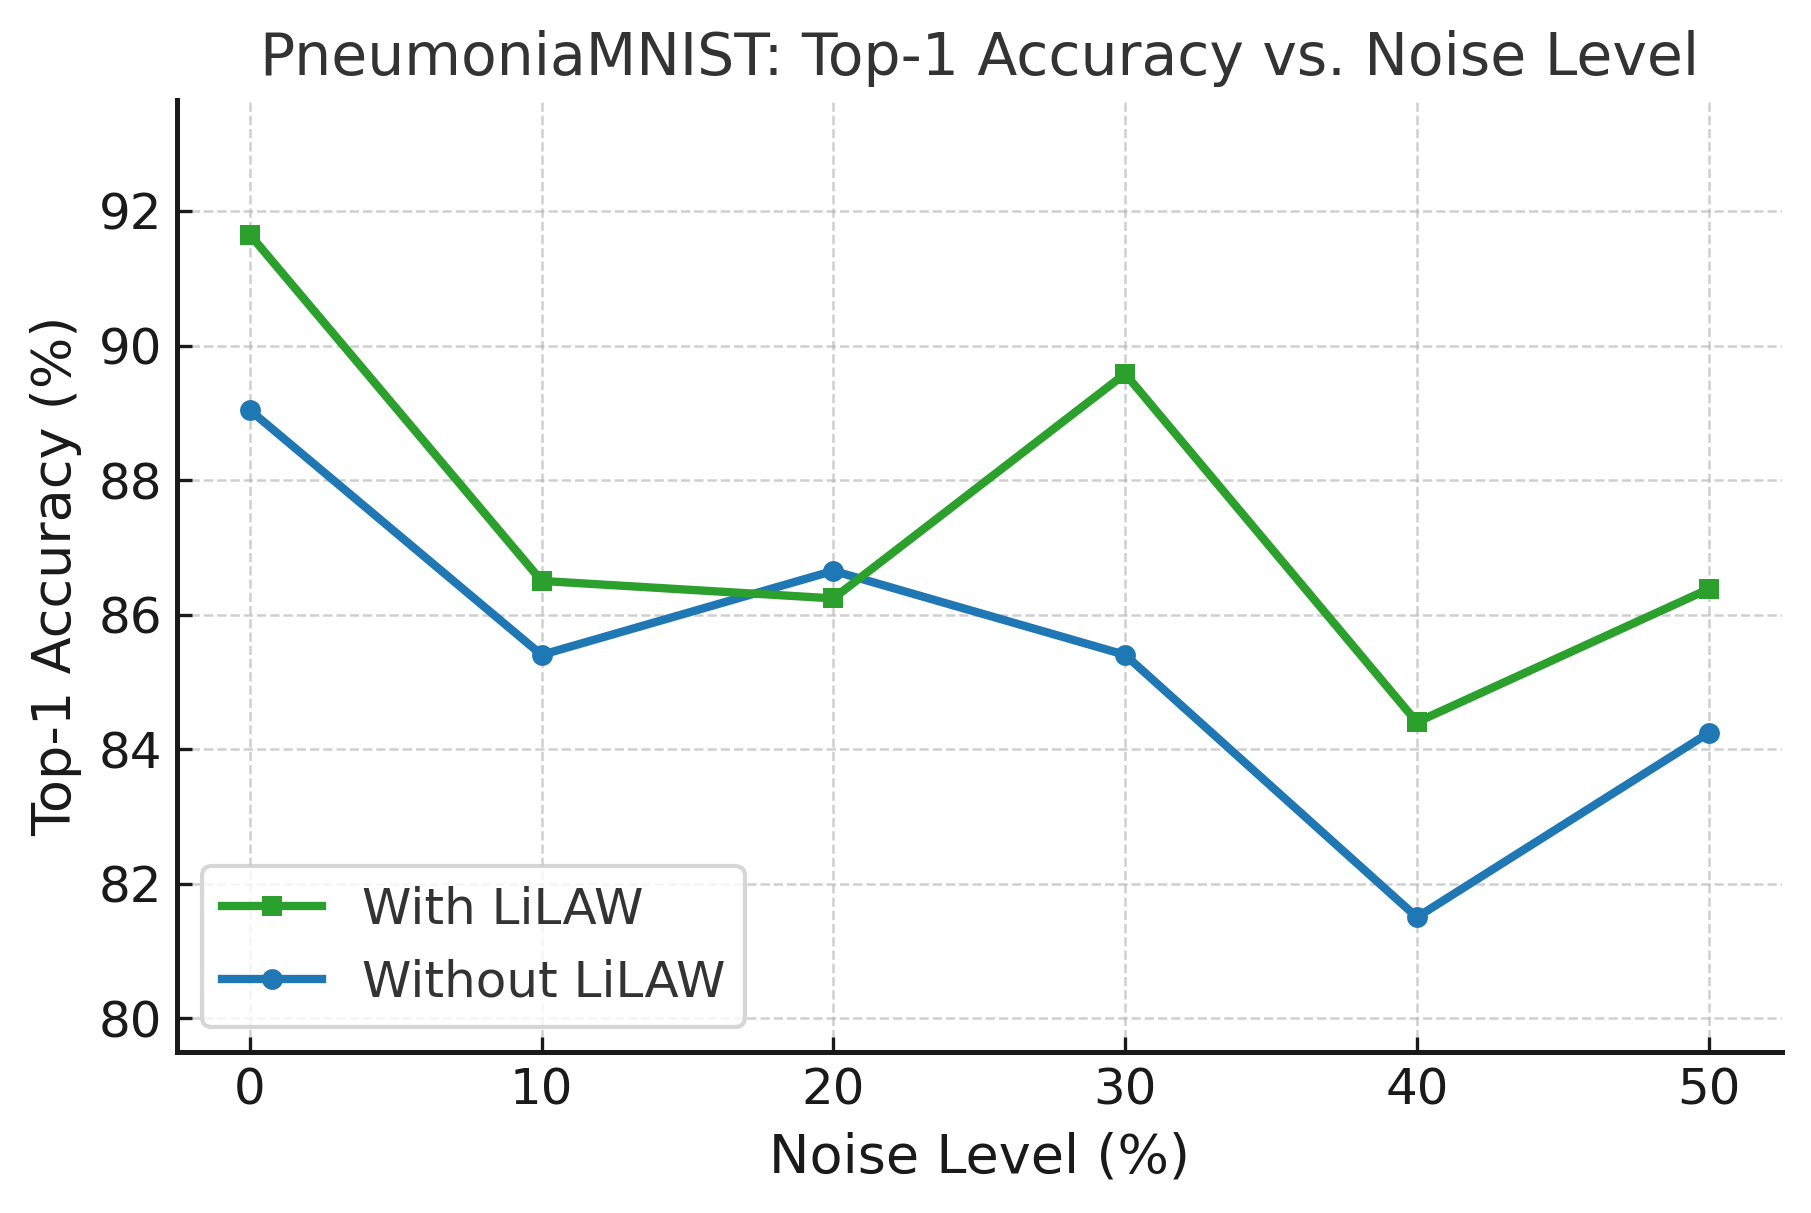
\includegraphics[scale=0.21]{pneumonia.png}
    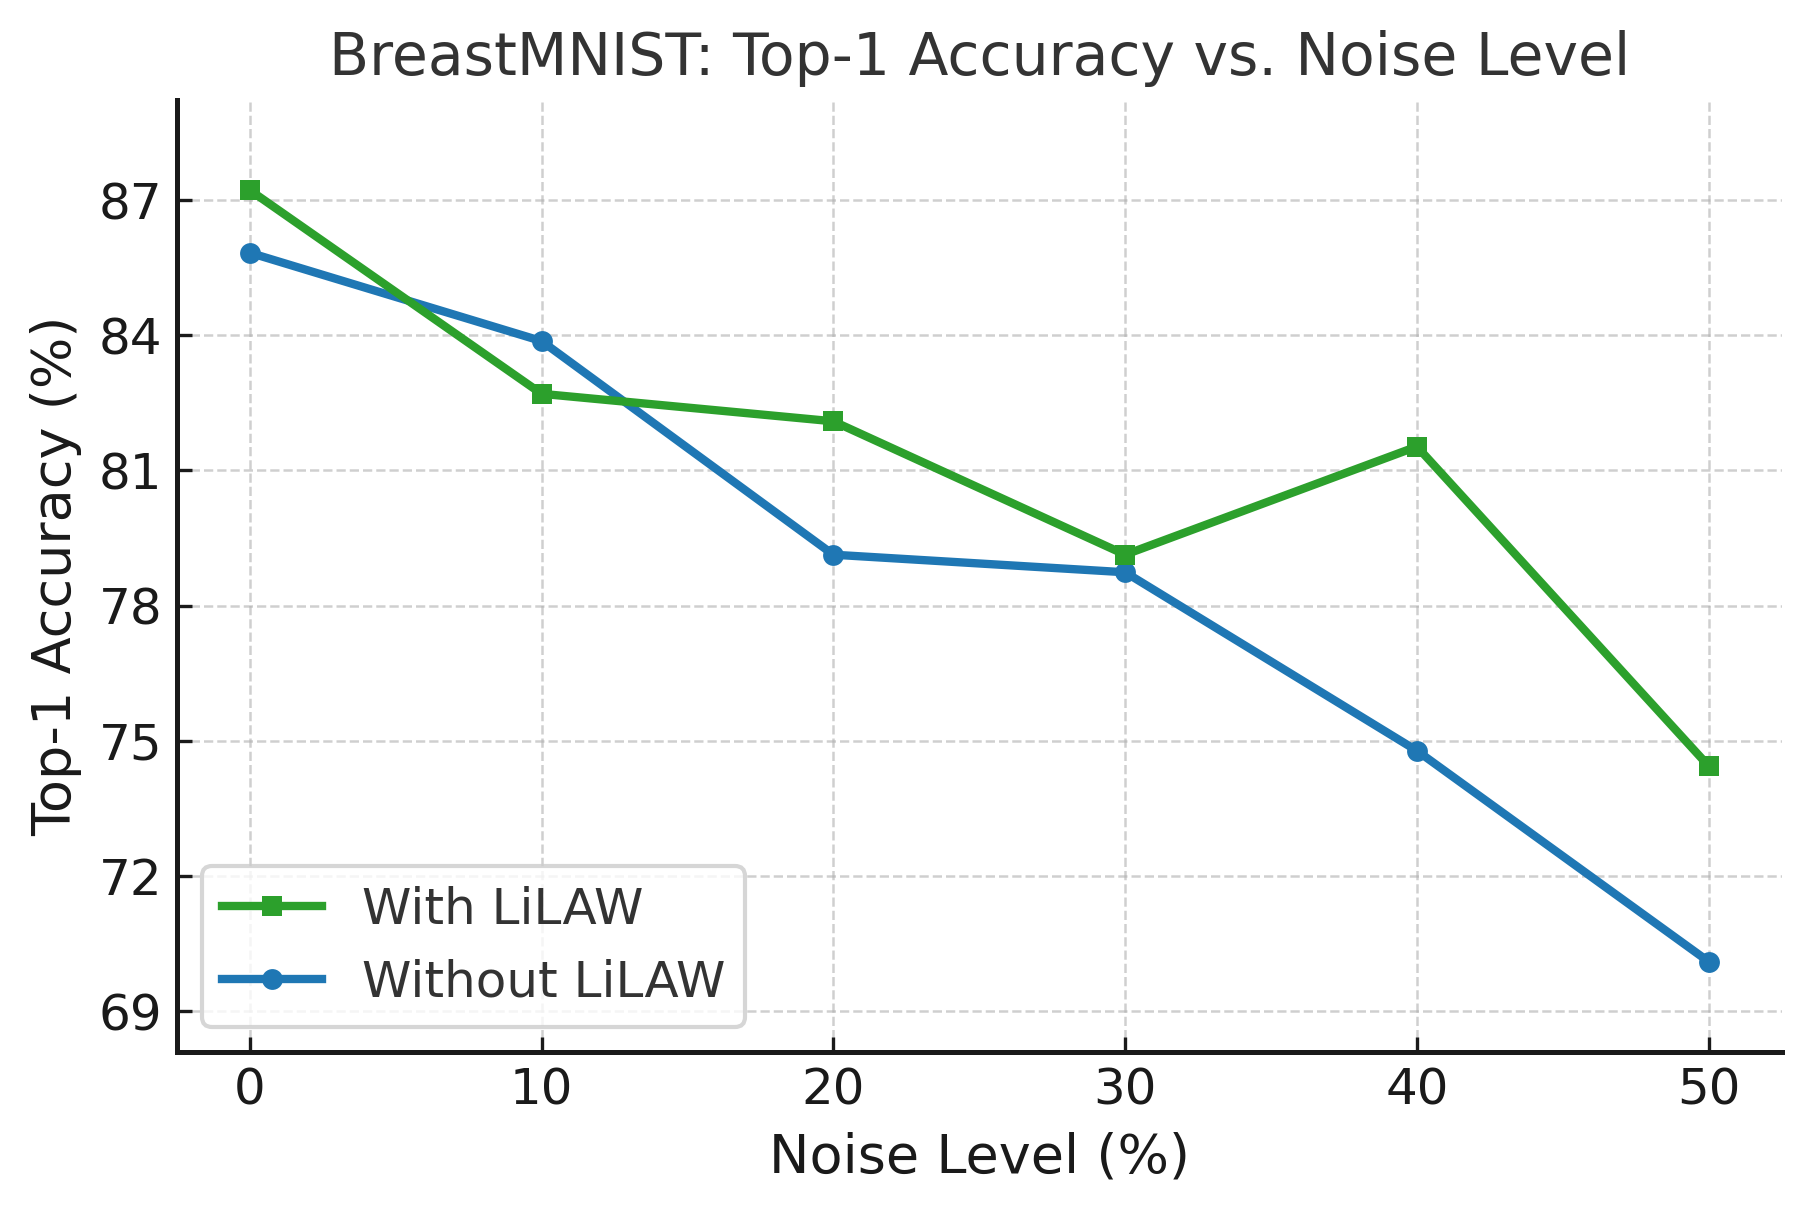
\includegraphics[scale=0.21]{breast.png}\\
    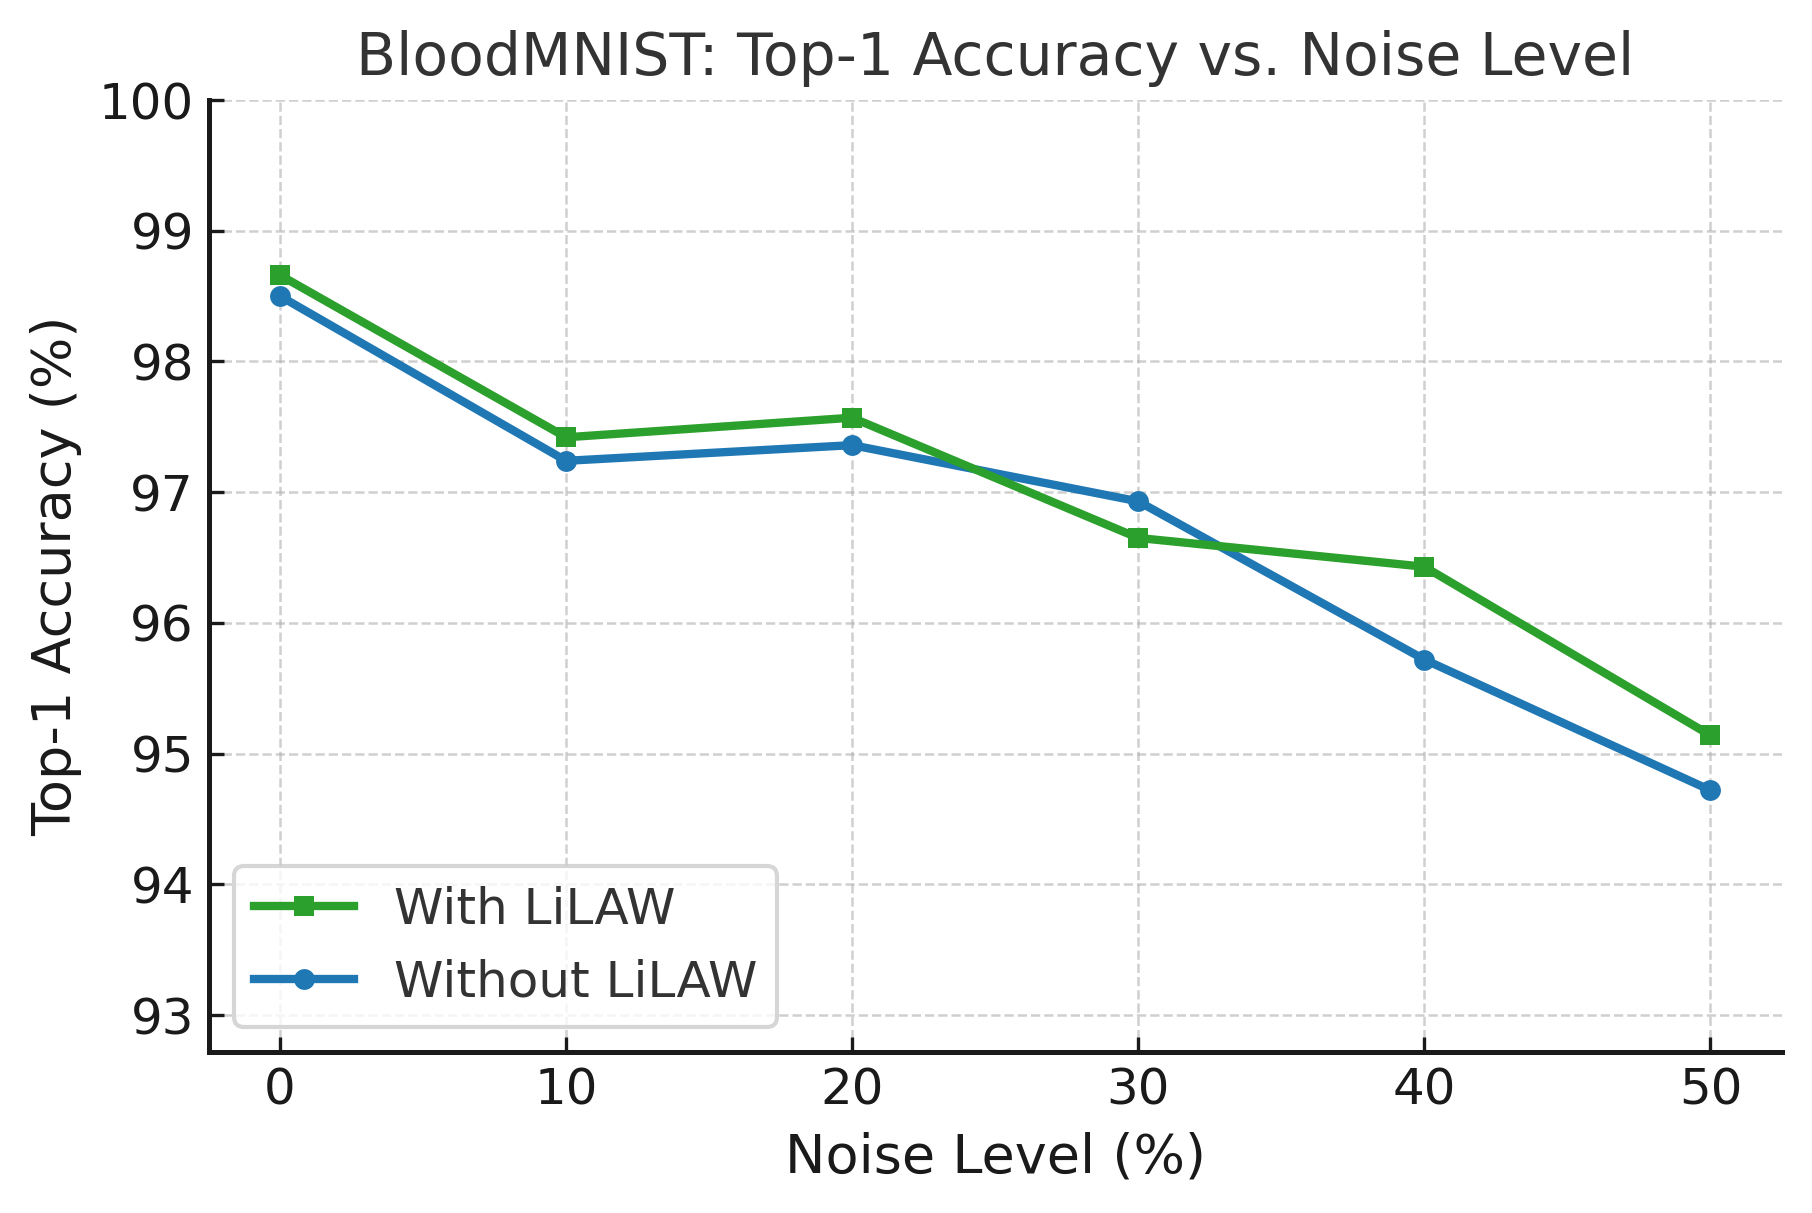
\includegraphics[scale=0.21]{blood.png}
    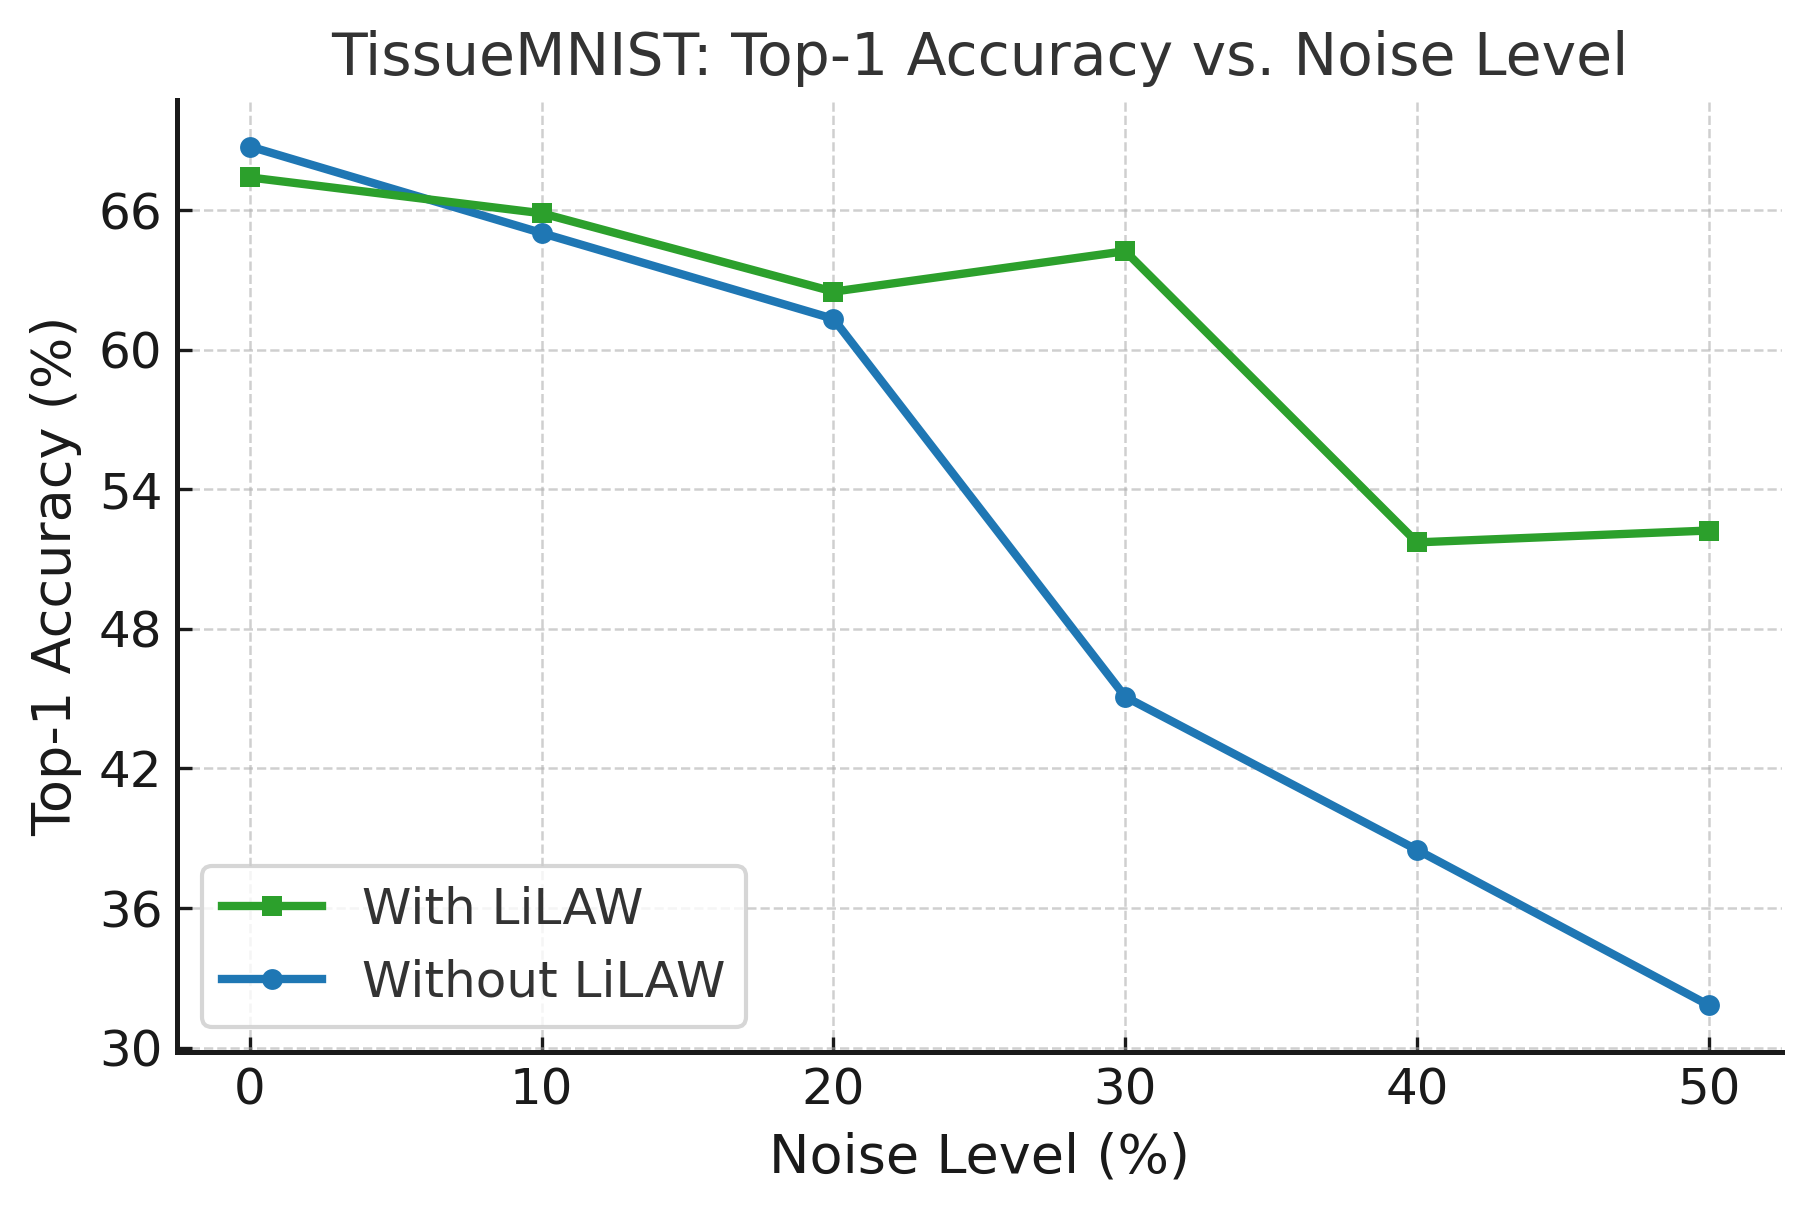
\includegraphics[scale=0.21]{tissue.png}
    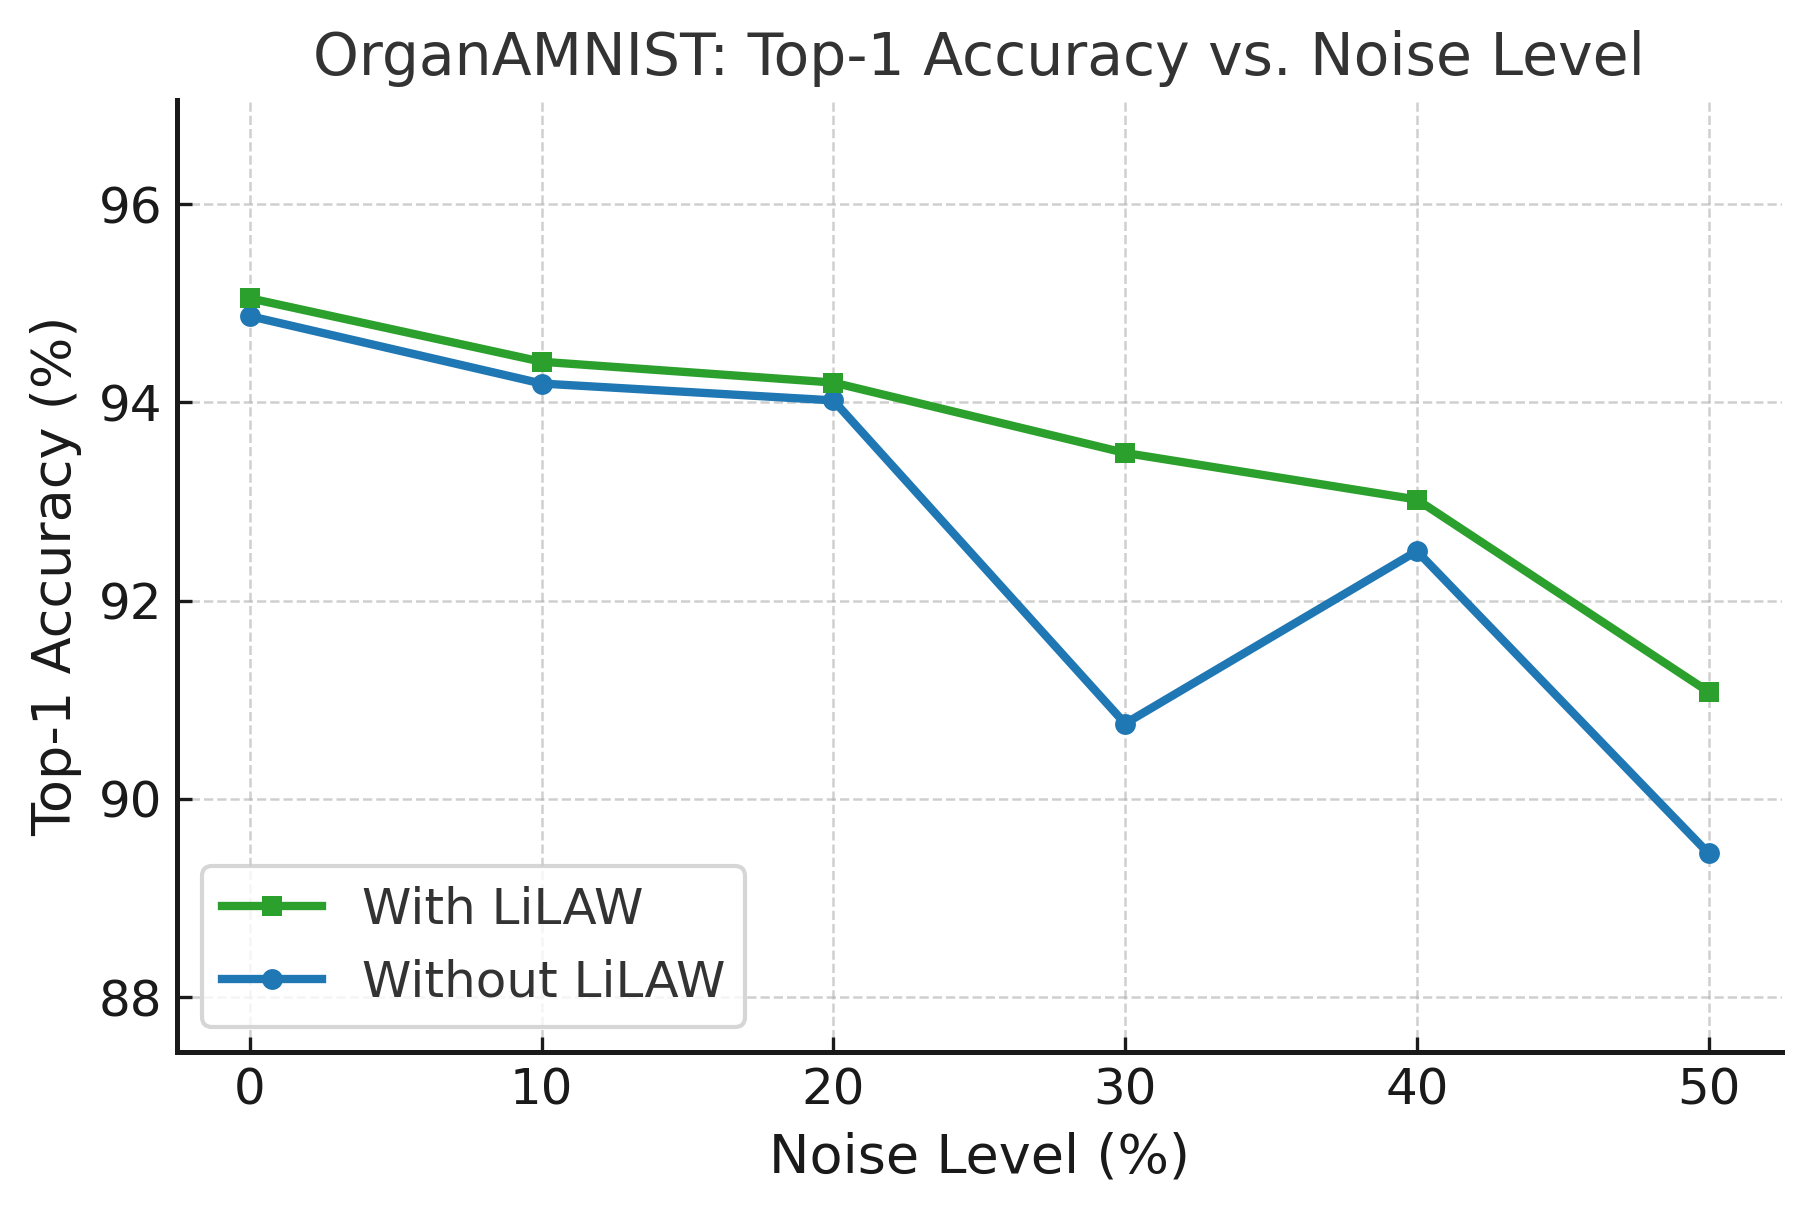
\includegraphics[scale=0.21]{organa.png}
    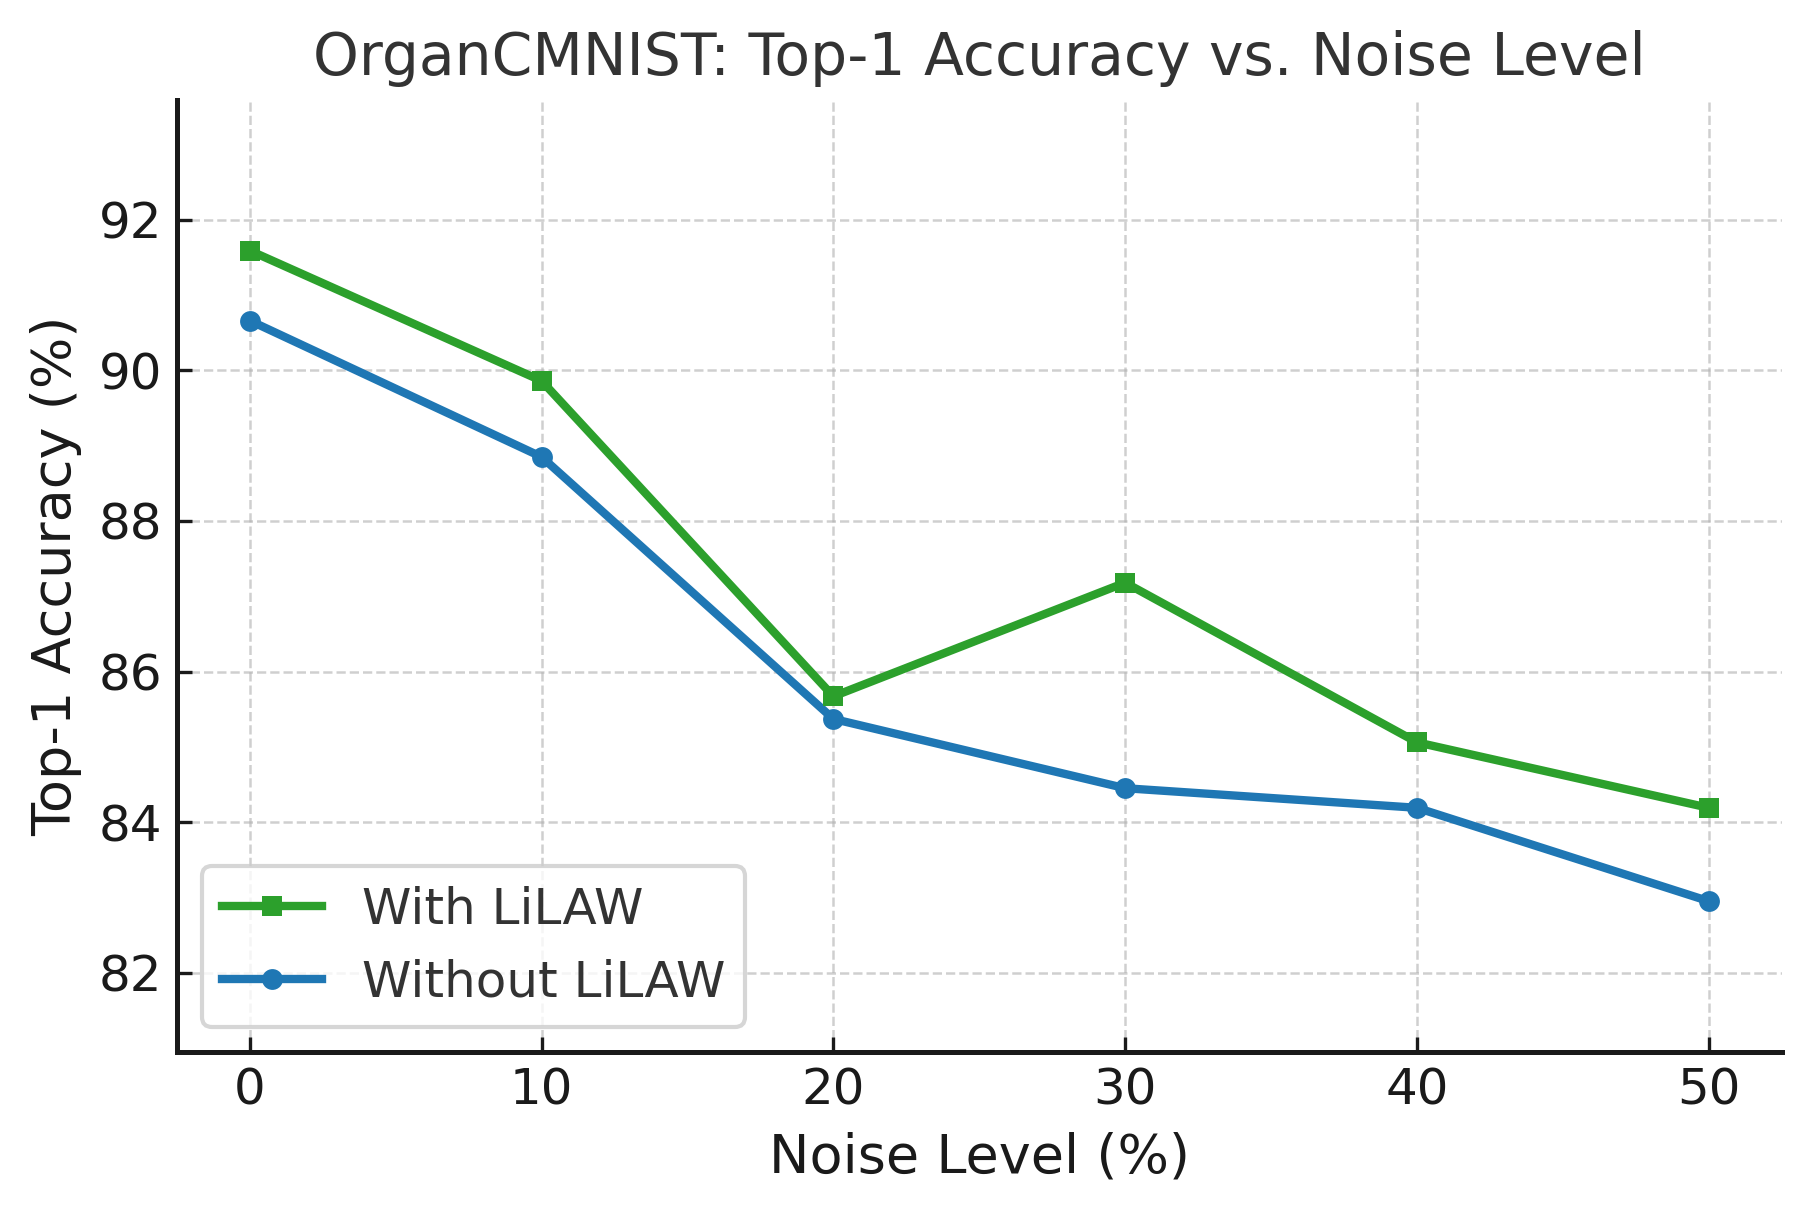
\includegraphics[scale=0.21]{organc.png}
    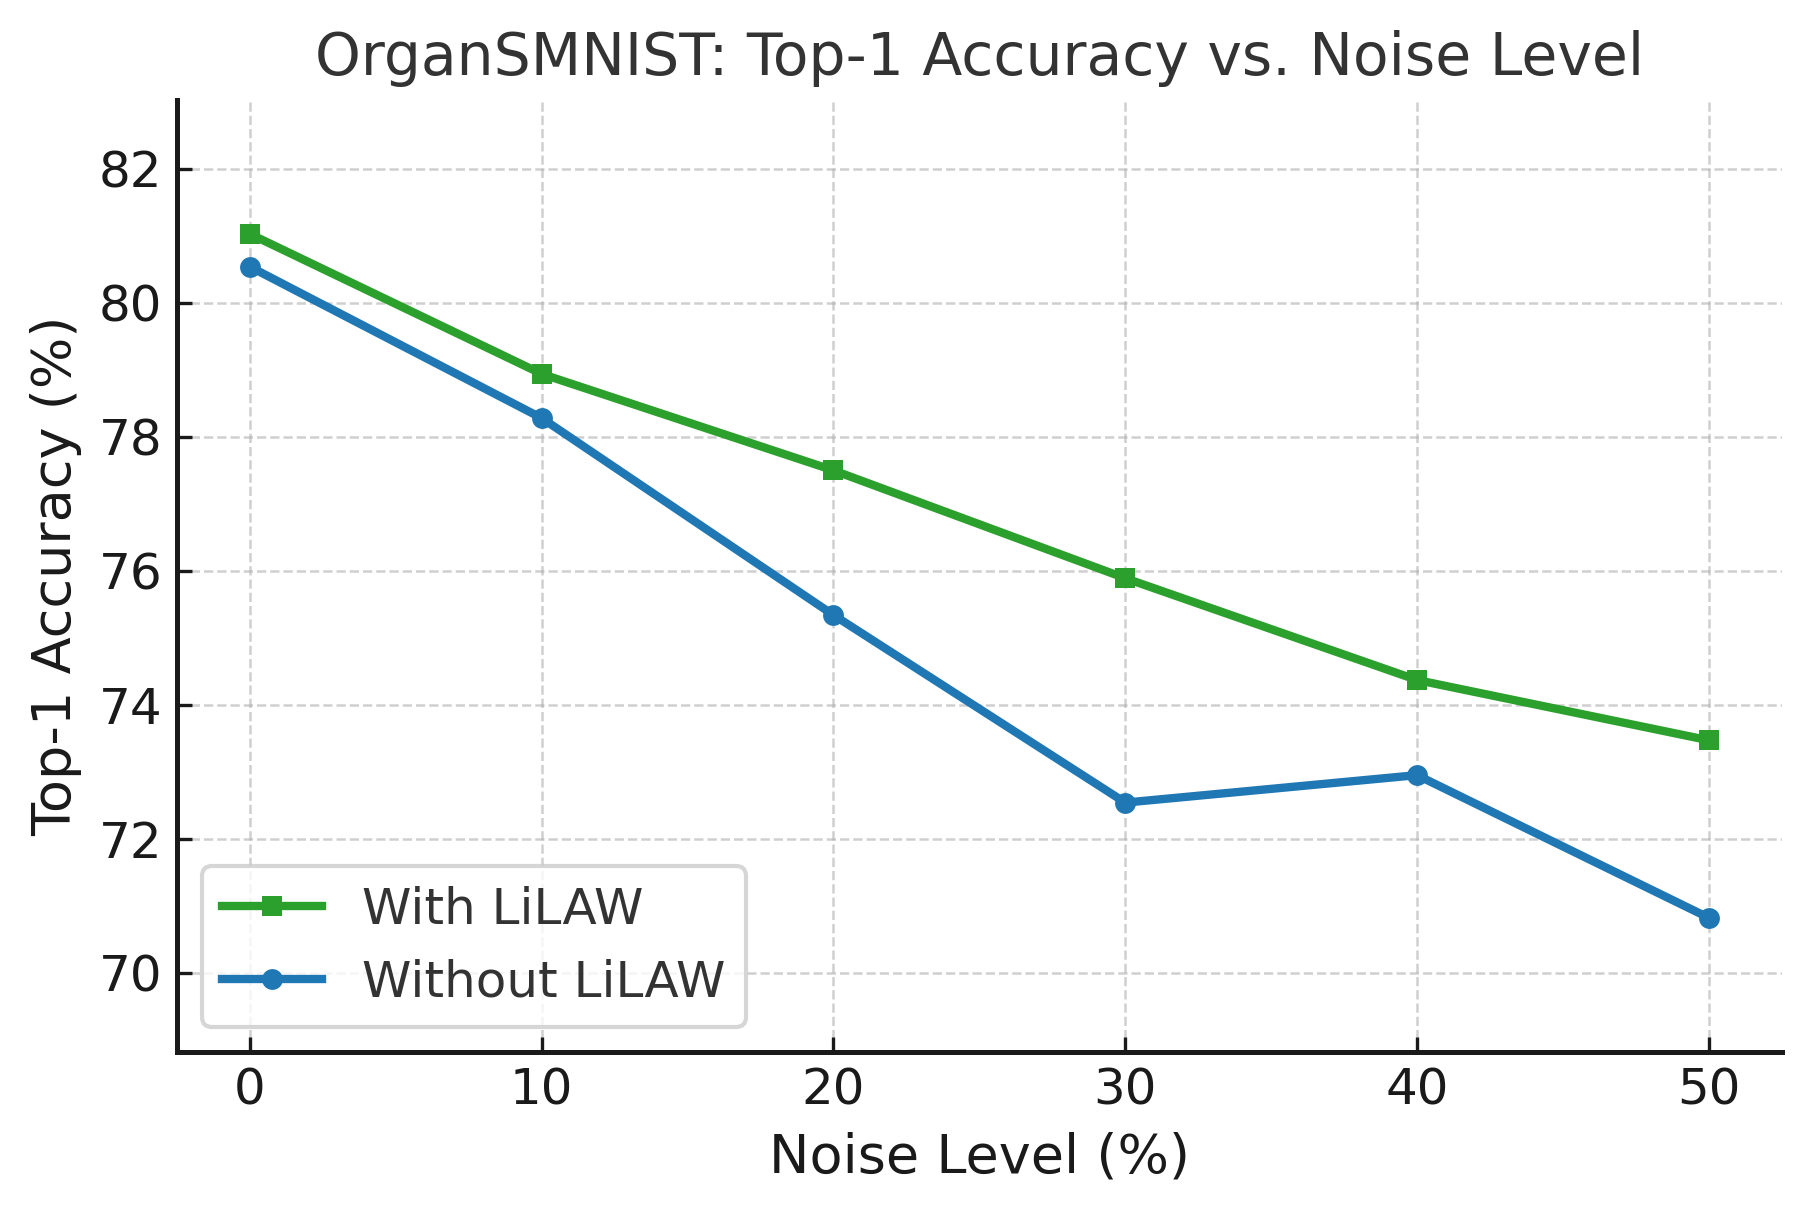
\includegraphics[scale=0.21]{organs.png}
    \caption{Accuracy with and without LiLAW on ten 2D datasets from MedMNISTv2.}
    \label{fig:med1}
    \vspace{-0.5em}
\end{figure*}

%Table~\ref{tab:ecg5000_results} highlights the effectiveness of LiLAW on ECG5000. Compared to standard training, LiLAW yields a substantial improvement in accuracy and AUROC, demonstrating its ability to enhance predictive performance and discrimination in inherently noisy domains. Namely, LiLAW can dynamically reweight samples based on difficulty to effectively mitigate the impact of inherent noise in physiological signals. This suggests that LiLAW provides a generalizable framework to improve robustness across modalities where label quality and data heterogeneity are common challenges.

\subsection{Performance Comparison: Identifying Mislabels}

LiLAW's high AUCROC \& AUCPRC values suggest that it is highly effective at identifying mislabeled samples at early-stage and late-stage training and consistently outperforms several methods for difficulty estimation, including Data-IQ~\citep{seedat_data-iq_2022}, DataMaps~\citep{swayamdipta_dataset_2020}, CNLCU-S~\citep{xia_sample_2021}, AUM~\citep{pleiss_identifying_2020}, EL2N~\citep{paul_deep_2023}, Grand~\citep{paul_deep_2023}, and Forgetting~\citep{toneva_empirical_2019} (see \ref{supp:comp}, Table \ref{table:comp}).

\subsection{Performance Comparison: Noisy-Label Learning}

Using the Clothing-1M dataset \citep{xiao2015learning}, a real-world noisy dataset, we evaluate LiLAW using ResNet-50 with ImageNet-21K pretraining. The same training method used in the 11 methods in Table~\ref{tab:noisy_label_results} (results obtained from the respective papers) was used with LiLAW. Several comparable noisy-label learning methods improve performance over standard cross-entropy, confirming their effectiveness in mitigating label corruption. Some methods however require substantially heavier training pipelines, pruning (worsening fairness), more data, or more models and are not directly comparable to our method. In contrast, our method achieves 71.44\% accuracy. This makes it competitive with many existing methods while maintaining a lightweight design without pruning or additional networks or prediction heads or computational overhead. This suggests LiLAW's practicality and scalability for real-world noisy-label settings. It is also important to note that the Clothing-1M dataset is \textbf{not} diagonally dominant in at least 2-3 classes~\cite{hedderich2021analysing}. Even so, our method improves performance.

\begin{table}[h!]
\centering
\begin{footnotesize}
\begin{tabular}{l|c}
\toprule
\textbf{Method} & \textbf{Accuracy (\%)} \\
\midrule
Cross-entropy & 69.21 \\
\midrule
Backward \citep{patrini2016making} & 69.13 \\
GCE \citep{zhang2018generalized} & 69.75 \\
Forward \citep{patrini2016making} & 69.84 \\
Co-teaching \citep{han2018co} & 70.15 \\
SEAL \citep{chen2021beyond} & 70.63 \\
SL \citep{wang2019symmetric} & 71.02 \\
Weakly Supervised \citep{zhang2019metacleaner} & 71.36 \\
LRT \citep{zheng2020error} & 71.74 \\
Joint-Optim \citep{tanaka2018joint} & 72.16 \\
MixNN \citep{lu2024mitigating} & 72.39 \\
MetaCleaner \citep{zhang2019metacleaner} & 72.50 \\ 
\midrule
LiLAW (ours) & 71.44 \\
\bottomrule
\end{tabular}
\caption{Noisy-label learning methods on Clothing-1M.}
\label{tab:noisy_label_results}
\end{footnotesize}
\vspace{-2.1em}
\end{table}

\subsection{Performance Comparison: Synthetic Datasets}
\label{sec:synthetic}

We achieve state-of-the-art results using LiLAW on the UofR dataset for pain detection with the incorporation of real data from UNBC and UofR and synthetic data from \synpain (see~\ref{sec:pain}, Table~\ref{x}). Also, we achieve state-of-the-art results using LiLAW on the PD-GaM dataset for gait classification with the incorporation of real data from the PD-GaM dataset and synthetic data from the \gaitgen dataset (see~\ref{sec:gait}, Table~\ref{tab:gait}). And finally, we achieve state-of-the-art results using LiLAW on the ECG5000 dataset using real data from ECG5000 and augmented data from ECG5000-A for heartbeat classification (see~\ref{sec:heart}, Table~\ref{tab:ecg}).

\subsection{Performance Comparison: Improving Fairness}
\label{sec:fairness}

Using LiLAW on the Adult dataset, we consistently improve overall performance (accuracy, average precision, recall, and F1-score). While the majority class benefits uniformly, the minority class has a small drop in recall for higher boost in precision and F1-score. Across sex, race, and age, LiLAW generally reduces disparities in demographic parity, equalized odds, and accuracy by implicitly giving more weight to harder samples (more common in disadvantaged groups), even though some trade-offs with predictive parity remain unavoidable. Further details and proof of fairness in~\ref{fairness}.
\vspace{-0.5em}
\section{Conclusion}
\label{sec:conclusion}
In this work, we introduced LiLAW, a simple, lightweight, adaptive weighting method that consistently improves training under noisy and heterogeneous conditions. By learning only three parameters that evolve with sample difficulty, LiLAW can be easily integrated into existing pipelines without added complexity, which is especially useful for data-constrained and resource-constrained settings. We highlight LiLAW's practical utility using medical, time-series, and synthetic data. It also helps with fairness, while handling imbalance more adaptively than static methods. LiLAW opens up opportunities for active learning (select difficult samples), continual learning (stabilize drift), and semi-supervised learning (deal with low-confidence pseudo-labels). 

\newpage

\section*{Impact Statement}
This paper presents work whose goal is to advance the field of machine learning. There are many potential societal consequences of our work, none of which we feel must be specifically highlighted here.

\section*{Acknowledgements}
We acknowledge the support of the Vector Institute for Artificial Intelligence, Ontario Graduate Scholarships, the Canadian Institutes of Health Research, the Natural Sciences and Engineering Research Council of Canada, and the University of Toronto.

\section*{Ethics Statement}
All datasets used in this work are publicly available and widely used for research purposes. This work does not present any known ethical concerns.

%\section*{Reproducibility Statement}

%The details provided about Datasets (see Section~\ref{sec:datasets}) and Models \& Implementation (see Section~\ref{sec:models}) along with the code provided in the Supplementary Material make this work reproducible.

\bibliography{example_paper}
\bibliographystyle{icml2026}

\newpage
\appendix
\onecolumn
\section{Appendix}
\label{supp}
\setcounter{section}{1}

\subsection{Motivating example}
\label{supp:example}

\begin{table}[ht] \centering \resizebox{\textwidth}{!}{
\begin{tabular}{l|c|c|c|c|ccccc|cccccc}
\toprule
Case (True Label is [1,0]) & Prediction & $s_y$ & $s_{\max}$ & CE
& \multicolumn{5}{c|}{$\alpha=10,\;\beta=2,\;\delta=6$} 
& \multicolumn{5}{c}{$\alpha=9,\;\beta=3,\;\delta=7$} \\
\cmidrule(lr){6-10} \cmidrule(lr){11-15}
&  &  &  &
 & $W_\alpha$ & $W_\delta$ & $W_\beta$ & $W$ & $\mathcal{L}_{W}$ 
 & $W_\alpha$ & $W_\delta$ & $W_\beta$ & $W$ & $\mathcal{L}_{W}$ \\
\midrule
Correct \& Confident     
 & [0.95,0.05] & 0.95 & 0.95 & \textbf{0.051}
& 0.999 & 0.199 & 0.500 & 1.698 & \textbf{0.087} 
& 0.999 & 0.000 & 0.130 & 1.129 & \textbf{0.058} \\
Correct \& Unconfident   
& [0.60,0.40] & 0.60 & 0.60 & \textbf{0.511}
 & 0.998 & 0.865 & 0.500 & 2.363 & \textbf{1.208} 
& 0.992 & 0.002 & 0.231 & 1.225 & \textbf{0.626} \\
Incorrect \& Unconfident 
 & [0.40,0.60] & 0.40 & 0.60 & \textbf{0.916}
 & 0.982 & 0.966 & 0.550 & 2.498 & \textbf{2.289} 
& 0.953 & 0.089 & 0.354 & 1.396 & \textbf{1.279} \\
Incorrect \& Confident   
 & [0.05,0.95] & 0.05 & 0.95 & \textbf{2.996}
 & 0.222 & 0.658 & 0.812 & 1.692 & \textbf{5.073} 
& 0.378 & 0.835 & 0.690 & 1.903 & \textbf{5.700} \\
\bottomrule
\end{tabular}}
\caption{Comparison of cross-entropy (CE) and LiLAW-weighted loss under two $\alpha,\beta,\delta$ settings.}
\label{tab:lilaw_toy}
\end{table}
\vspace{-1em}
As shown in Table~\ref{tab:lilaw_toy}, LiLAW adapts weighting beyond what CE alone provides. When predictions are correct and confident, LiLAW assigns relatively small weights, keeping the loss close to CE and preventing overfitting. When predictions are correct but unconfident, LiLAW amplifies the loss and gives importance to samples that CE might undervalue. When predictions are incorrect but unconfident, LiLAW boosts the loss to ensure that the model learns from these ambiguous samples. When predictions are incorrect and confident, LiLAW increases the penalty, discouraging the network from becoming overconfident in wrong answers. The main benefit of LiLAW comes from the dynamic nature of $\alpha,\beta,\delta$. If $\alpha=10\rightarrow 9$, $\beta=2 \rightarrow 3$, and $\delta=6\rightarrow 7$, then whereas CE still has the same penalties for the cases if they are seen again, LiLAW further decreases the penalty on the correct cases and unconfident cases, while increasing the penalty on the incorrect and confident cases, which causes the incorrect and confident cases to self-correct more effectively.

\subsection{Diagonally Dominant Noise}
\label{proof:diag}

Learning a reliable model under label noise with no assumptions about the noise transition matrix, which describes how labels are corrupted, is usually unrealistic. That said, \textit{our method does not require estimating this matrix or using it directly}. It only assumes a mild property of the noise transition matrix. A common assumption is that the noise is diagonally dominant~\citep{han2018co, yu2019does}, meaning that for each class, a sample is more likely to keep its true label than to be flipped to any one other class. This is different from assuming that the noise rate is below 50\% for every class. Even if more than half of the labels are wrong in a given class, the correct label can still be the most likely outcome when mistakes are spread across many different wrong classes. 

Under diagonally dominant noise, even when the learned model is only close to the optimal noisy-data classifier, \citet{gui2021towards} prove that examples whose observed label is actually correct tend to align better with the input patterns, so a reasonably trained model will usually assign them lower loss than mislabeled examples that share the same observed label. In practice, pruning can find a mostly clean subset and loss-based reweighting can downweigh mostly clean samples and upweigh noisier samples to potentially correct them. This is why both pruning-based and reweighting-based approaches often perform well under diagonally dominant noise.

\subsubsection{Proof that diagonally dominant noise is sufficient for LiLAW}

% Sigmoid:
\newcommand{\sigmoid}{\sigma}
\newcommand{\CE}{\ell_{\mathrm{CE}}}

We prove a corollary to Theorems~1 and 2 in~\citet{gui2021towards}, with a similar setup, to show that diagonally dominant noise is sufficient for LiLAW.

\begin{corollary}
Let $c\ge 2$ and assume label noise with transition matrix
$T\in[0,1]^{c\times c}$ where $T_{ij} := \mathbb{P}(\tilde y=j \mid y=i)$.
Assume the diagonally dominant condition used in Theorems~1 and 2 in \citet{gui2021towards}:
\begin{equation}
\label{eq:dd}
T_{ii} > \max\Bigl\{\max_{j\neq i} T_{ij},\ \max_{j\neq i} T_{ji}\Bigr\}\qquad \forall i\in\{0,\dots,c-1\}.
\end{equation}
Let $(x,\tilde y)$ be an input and observed label pair, let $f^*(x)\in\{0,\dots,c-1\}$ be the true label function (referred to as the target concept in~\citet{gui2021towards}), let $g^*(x)$ be the deep neural network minimizing the expected loss, and let $s=\mathrm{softmax}(g(x))$.
For LiLAW parameters $(\alpha,\beta,\delta)$, we define the per-sample LiLAW weight as in Sec.~\ref{sec:method}:
\begin{align}
    \mathcal{W}_\alpha (s, \tilde{y}) = \sigma(\alpha \cdot s[\tilde{y}] - \max(s))
\end{align}
\begin{align}
    \mathcal{W}_\beta (s, \tilde{y}) = \sigma(-(\beta \cdot s[\tilde{y}] - \max(s)))
\end{align}
\begin{align}
    \mathcal{W}_\delta (s, \tilde{y}) = \exp\biggl(-\frac{(\delta \cdot s[\tilde{y}] - \max(s))^2}{2}\biggr)
\end{align}

\noindent We calculate the weight for each sample as follows:
\begin{align}
    \mathcal{W}(s, \tilde{y}) = \mathcal{W}_\alpha (s, \tilde{y}) + \mathcal{W}_\beta (s, \tilde{y}) + \mathcal{W}_\delta (s, \tilde{y})
\end{align}

\noindent and define our LiLAW (weighted) loss function, in our case, $\ell$ is cross-entropy loss, as follows:
\begin{equation}
\label{eq:lilaw-loss}
\mathcal{L}_{W} = \mathcal{W}(s, \tilde{y}) \cdot \ell(g^*(x), \tilde{y})
\end{equation}

Fix any observed label $\tilde{y}$ and consider two points $(x_c,\tilde y)$ and $(x_n,\tilde y)$
with the same observed label, where $f^*(x_c)=\tilde y$ (clean label) and
$f^*(x_n)=i\neq \tilde y$ (noisy label).
Then, under diagonally dominant noise \eqref{eq:dd}, the following hold:
\begin{enumerate}[label=(\roman*),leftmargin=*]
\item \textbf{(Loss separates clean and noisy samples)} unweighted clean label loss is less than unweighted noisy label loss:
\[
\ell(g^*(x_c),\tilde y) < \ell(g^*(x_n),\tilde y)
\]
\item \textbf{(LiLAW geometry separates clean and noisy samples)} disagreement is 0 for clean labels and $> 0$ for noisy labels:
\[
m(x,\tilde y) = \max(s) - s[\tilde y] \implies m(x_c,\tilde y)=0 \wedge m(x_n,\tilde y)=T_{ii}-T_{i\tilde y}>0
\]
\item \textbf{(LiLAW weights separate clean and noisy samples)} if $\alpha\ge 1$ and $\beta\ge 1$, then:
\[
\mathcal{W}_{\alpha}(s(x_c),\tilde y) \;>\; \mathcal{W}_{\alpha}(s(x_n),\tilde y)
\qquad\text{and}\qquad
\mathcal{W}_{\beta}(s(x_c),\tilde y) \;<\; \mathcal{W}_{\beta}(s(x_n),\tilde y).
\]
\end{enumerate}
Consequently, diagonal dominance is sufficient to guarantee that the LiLAW values, $s[\tilde y]$ and $\max(s))$, and the LiLAW weights $\mathcal{W}_{\alpha},\mathcal{W}_{\beta},\mathcal{W}_{\delta}$ contain a strict clean vs.\ noisy separation signal for samples sharing the same observed label.
\end{corollary}

\begin{proof}
By Lemma~2 (used in the proof of Theorems~1 and 2 in the Appendix of~\cite{gui2021towards}), the deep neural network $g^*$ minimizing the expected loss satisfies:
\begin{equation}
\label{eq:gstar-row}
s(g^*(x))[j] = T_{f^*(x),j}\qquad \forall j.
\end{equation}

\noindent\emph{(i)}
If $f^*(x_c)=\tilde y$, then by \eqref{eq:gstar-row} we have $s(g^*(x_c))[\tilde y]=T_{\tilde y\tilde y}$.
If $f^*(x_n)=i\neq \tilde y$, then $s(g^*(x_n))[\tilde y]=T_{i\tilde y}$.

Since diagonal dominance \eqref{eq:dd} implies $T_{\tilde y\tilde y} > T_{i\tilde y} \implies -\log T_{\tilde y\tilde y} < -\log T_{i\tilde y} \implies \ell(g^*(x_c),\tilde y) < \ell(g^*(x_n),\tilde y)$.

\noindent\emph{(ii)}
For $x_c$ with true label $\tilde y$, \eqref{eq:gstar-row} and diagonal dominance \eqref{eq:dd} imply
\[
\max_j s(g^*(x_c))[j] = \max_j T_{\tilde y j} = T_{\tilde y\tilde y} = s(g^*(x_c))[\tilde y] \implies m(x_c,\tilde y)=0
\]
For $x_n$ with true label $i\neq \tilde y$, \eqref{eq:gstar-row} and diagonal dominance \eqref{eq:dd} imply
\[
\max_j s(g^*(x_n))[j] = \max_j T_{i j} = T_{ii} \text{ and } s(g^*(x_n))[\tilde y]=T_{i\tilde y} \implies m(x_n,\tilde y)=T_{ii}-T_{i\tilde y}>0 \text{ since } T_{ii}>\max_{j\neq i}T_{ij}\ge T_{i\tilde y}
\]

\noindent\emph{(iii)}
Because the sigmoid function is strictly increasing, it suffices to compare its arguments.

Let $s_c=s(g^*(x_c))[\tilde y]=T_{\tilde y\tilde y}$, $s_n=s(g^*(x_n))[\tilde y]=T_{i\tilde y}$, $M_c=\max_j s(g^*(x_c))[j]=s_c$, $M_n=\max_j s(g^*(x_n))[j]=T_{ii}$.

Then,
\begin{align*}
\bigl(\alpha s_c - M_c\bigr) - \bigl(\alpha s_n - M_n\bigr)
&= \alpha(s_c-s_n) - (M_c-M_n) \\
&= (\alpha-1)(s_c-s_n) + (M_n-s_n).
\end{align*}
Under \eqref{eq:dd}, we have $s_c>s_n$ and $M_n-s_n=T_{ii}-T_{i\tilde y}>0$,
so for $\alpha\ge 1$, $\mathcal{W}_{\alpha}(s(x_c),\tilde y)>\mathcal{W}_{\alpha}(s(x_n),\tilde y)$.

Similarly,
\begin{align*}
\bigl(M_n-\beta s_n\bigr) - \bigl(M_c-\beta s_c\bigr)
&= (M_n-M_c) - \beta(s_n-s_c) \\
&= (M_n-s_n) + (\beta-1)(s_c-s_n).
\end{align*}
Again, we have $M_n-s_n>0$ and $s_c-s_n>0$, so for $\beta\ge 1$, $\mathcal{W}_{\beta}(s(x_c),\tilde y)<\mathcal{W}_{\beta}(s(x_n),\tilde y)$.

Since \emph{(i), (ii), and (iii)} hold, we have shown that it is possible to separate (and appropriately weigh) correctly labeled samples and incorrectly labeled samples using LiLAW under the condition that we have diagonally dominant noise.

\end{proof}

\subsection{Derivatives of weight functions}
\label{supp:derivative}

We consider the derivatives of our weight functions based on $\alpha, \beta, \delta$ with respect to the LiLAW weighted loss function to study how they grow with those three parameters. Note that our weight functions are defined as in Sec.~\ref{sec:method}:
\begin{align}
    \mathcal{W}_\alpha (s_i, \widetilde{y_i}) = \sigma(\alpha \cdot s_i[\widetilde{y_i}] - \max(s_i))\nonumber
\end{align}
\begin{align}
    \mathcal{W}_\beta (s_i, \widetilde{y_i}) = \sigma(-(\beta \cdot s_i[\widetilde{y_i}] - \max(s_i)))\nonumber
\end{align}
\begin{align}
    \mathcal{W}_\delta (s_i, \widetilde{y_i}) = \exp\biggl(-\frac{(\delta \cdot s_i[\widetilde{y_i}] - \max(s_i))^2}{2}\biggr)\nonumber
\end{align}
\noindent We calculated the weight for each sample as follows:
\begin{align}
    \mathcal{W}(s_i, \widetilde{y_i}) = \mathcal{W}_\alpha (s_i, \widetilde{y_i}) + \mathcal{W}_\beta (s_i, \widetilde{y_i}) + \mathcal{W}_\delta (s_i, \widetilde{y_i})\nonumber
\end{align}
\noindent and defined our LiLAW weighted loss function as follows:
\begin{align}
\mathcal{L}_{W} &= \mathcal{W}(s_i, \widetilde{y_i}) \cdot \mathcal{L}\nonumber
\end{align}
\noindent Based on the above definitions, we have the following derivatives:
\begin{align}
    \nabla_{\alpha}\mathcal{L}_{W} &= \diffp{\mathcal{L}_{W}}{\alpha} = \diffp{}{\alpha} (\mathcal{W}_\alpha (s_i, \widetilde{y_i}) \cdot \mathcal{L}) \nonumber = \mathcal{L} \cdot \diffp{}{\alpha} \mathcal{W}_\alpha (s_i, \widetilde{y_i}) \nonumber \\ &= \mathcal{L} \cdot \diffp{}{\alpha} (\sigma(\alpha \cdot s_i[\widetilde{y_i}] - \max(s_i))) \nonumber \\ &= \frac{\mathcal{L} \cdot (\sigma(\alpha \cdot s_i[\widetilde{y_i}] - \max(s_i)))^2 \cdot s_i[\widetilde{y_i}]}{\exp\biggl(\alpha \cdot s_i[\widetilde{y_i}] - \max(s_i)\biggl)}\nonumber \\ &= \frac{\mathcal{L} \cdot \mathcal{W}_\alpha (s_i, \widetilde{y_i})^2 \cdot s_i[\widetilde{y_i}]}{\exp\biggl(\alpha \cdot s_i[\widetilde{y_i}] - \max(s_i)\biggl)}\nonumber
\end{align}
\noindent Note: $\nabla_{\alpha}\mathcal{L}_{W} \geq 0$ as $\mathcal{L} \geq 0$, $\mathcal{W}_\alpha (s_i, \widetilde{y_i})^2 > 0$, $s_i[\widetilde{y_i}] \geq 0$, and $\exp\biggl(\alpha \cdot s_i[\widetilde{y_i}] - \max(s_i)\biggl) > 0$.

\begin{align}
    \nabla_{\beta}\mathcal{L}_{W} &= \diffp{\mathcal{L}_{W}}{\beta} = \diffp{}{\beta} (\mathcal{W}_\beta (s_i, \widetilde{y_i}) \cdot \mathcal{L})= \mathcal{L} \cdot \diffp{}{\beta} \mathcal{W}_\beta (s_i, \widetilde{y_i}) \nonumber \\ &= \mathcal{L} \cdot \diffp{}{\beta} (\sigma(-(\beta \cdot s_i[\widetilde{y_i}] - \max(s_i)))) \nonumber \\ &= -\frac{\mathcal{L} \cdot (\sigma(-(\beta \cdot s_i[\widetilde{y_i}] - \max(s_i))))^2 \cdot s_i[\widetilde{y_i}]}{\exp\biggl(-(\beta \cdot s_i[\widetilde{y_i}] - \max(s_i))\biggl)}\nonumber \\ &= -\frac{\mathcal{L} \cdot \mathcal{W}_\beta (s_i, \widetilde{y_i})^2 \cdot s_i[\widetilde{y_i}]}{\exp\biggl(-(\beta \cdot s_i[\widetilde{y_i}] - \max(s_i))\biggl)}\nonumber
\end{align}
\noindent Note: $\nabla_{\beta}\mathcal{L}_{W} \leq 0$ as $\mathcal{L} \geq 0$, $\mathcal{W}_\beta (s_i, \widetilde{y_i})^2 > 0$, $s_i[\widetilde{y_i}] \geq 0$, and $\exp\biggl(-(\beta \cdot s_i[\widetilde{y_i}] - \max(s_i))\biggl) > 0$.
\begin{align}\nabla_{\delta}\mathcal{L}_{W} &= \diffp{\mathcal{L}_{W}}{\delta} = \diffp{}{\delta} (\mathcal{W}_\delta (s_i, \widetilde{y_i}) \cdot \mathcal{L}) = \mathcal{L} \cdot \diffp{}{\delta} \mathcal{W}_\delta (s_i, \widetilde{y_i}) \nonumber \\ &= \mathcal{L} \cdot \diffp{}{\delta} \biggl(\exp\biggl(-\frac{(\delta \cdot s_i[\widetilde{y_i}] - \max(s_i))^2}{2}\biggr)\biggr) \nonumber \\ &= -\frac{\mathcal{L} \cdot (\delta \cdot s_i[\widetilde{y_i}] - \max(s_i)) \cdot s_i[\widetilde{y_i}]}{\exp\biggl(\frac{(\delta \cdot s_i[\widetilde{y_i}] - \max(s_i))^2}{2}\biggr)}\nonumber \\ &= -\mathcal{L} \cdot \mathcal{W}_\delta (s_i, \widetilde{y_i}) \cdot (\delta \cdot s_i[\widetilde{y_i}] - \max(s_i)) \cdot s_i[\widetilde{y_i}]\nonumber
\end{align}
\noindent Note: $\mathcal{L} \geq 0$, $\mathcal{W}_\delta (s_i, \widetilde{y_i})^2 > 0$, and $s_i[\widetilde{y_i}] \geq 0$, we see that $\nabla_{\delta}\mathcal{L}_{W} \leq 0$ when $\delta \cdot s_i[\widetilde{y_i}] \geq \max(s_i)$ and $\nabla_{\delta}\mathcal{L}_{W} > 0$ when $\delta \cdot s_i[\widetilde{y_i}] < \max(s_i)$.

In summary, the gradients for the parameters are updated using autograd, but we show why $\alpha$ always decreases and $\beta$ always increases at different rates. On the other hand, $\delta$ could increase or decrease depending on the conditions above. This is the reason for our choice of high $\alpha$, low $\beta$, and $\delta$ in between (by default, $\alpha=10,\beta=2,\delta=6$). Figure~\ref{fig:abd} shows that $\alpha$ decreases, $\beta$ increases, and $\delta$ increases as discussed above. The reason $\alpha$ decreases faster, $\delta$ increases faster, and $\beta$ increases faster with 50\% noise than 0\% noise is because easy samples are less reliable sooner, moderate cases are more informative faster, and hard samples are also more informative faster, respectively.

\begin{figure}[h!]
    \centering
    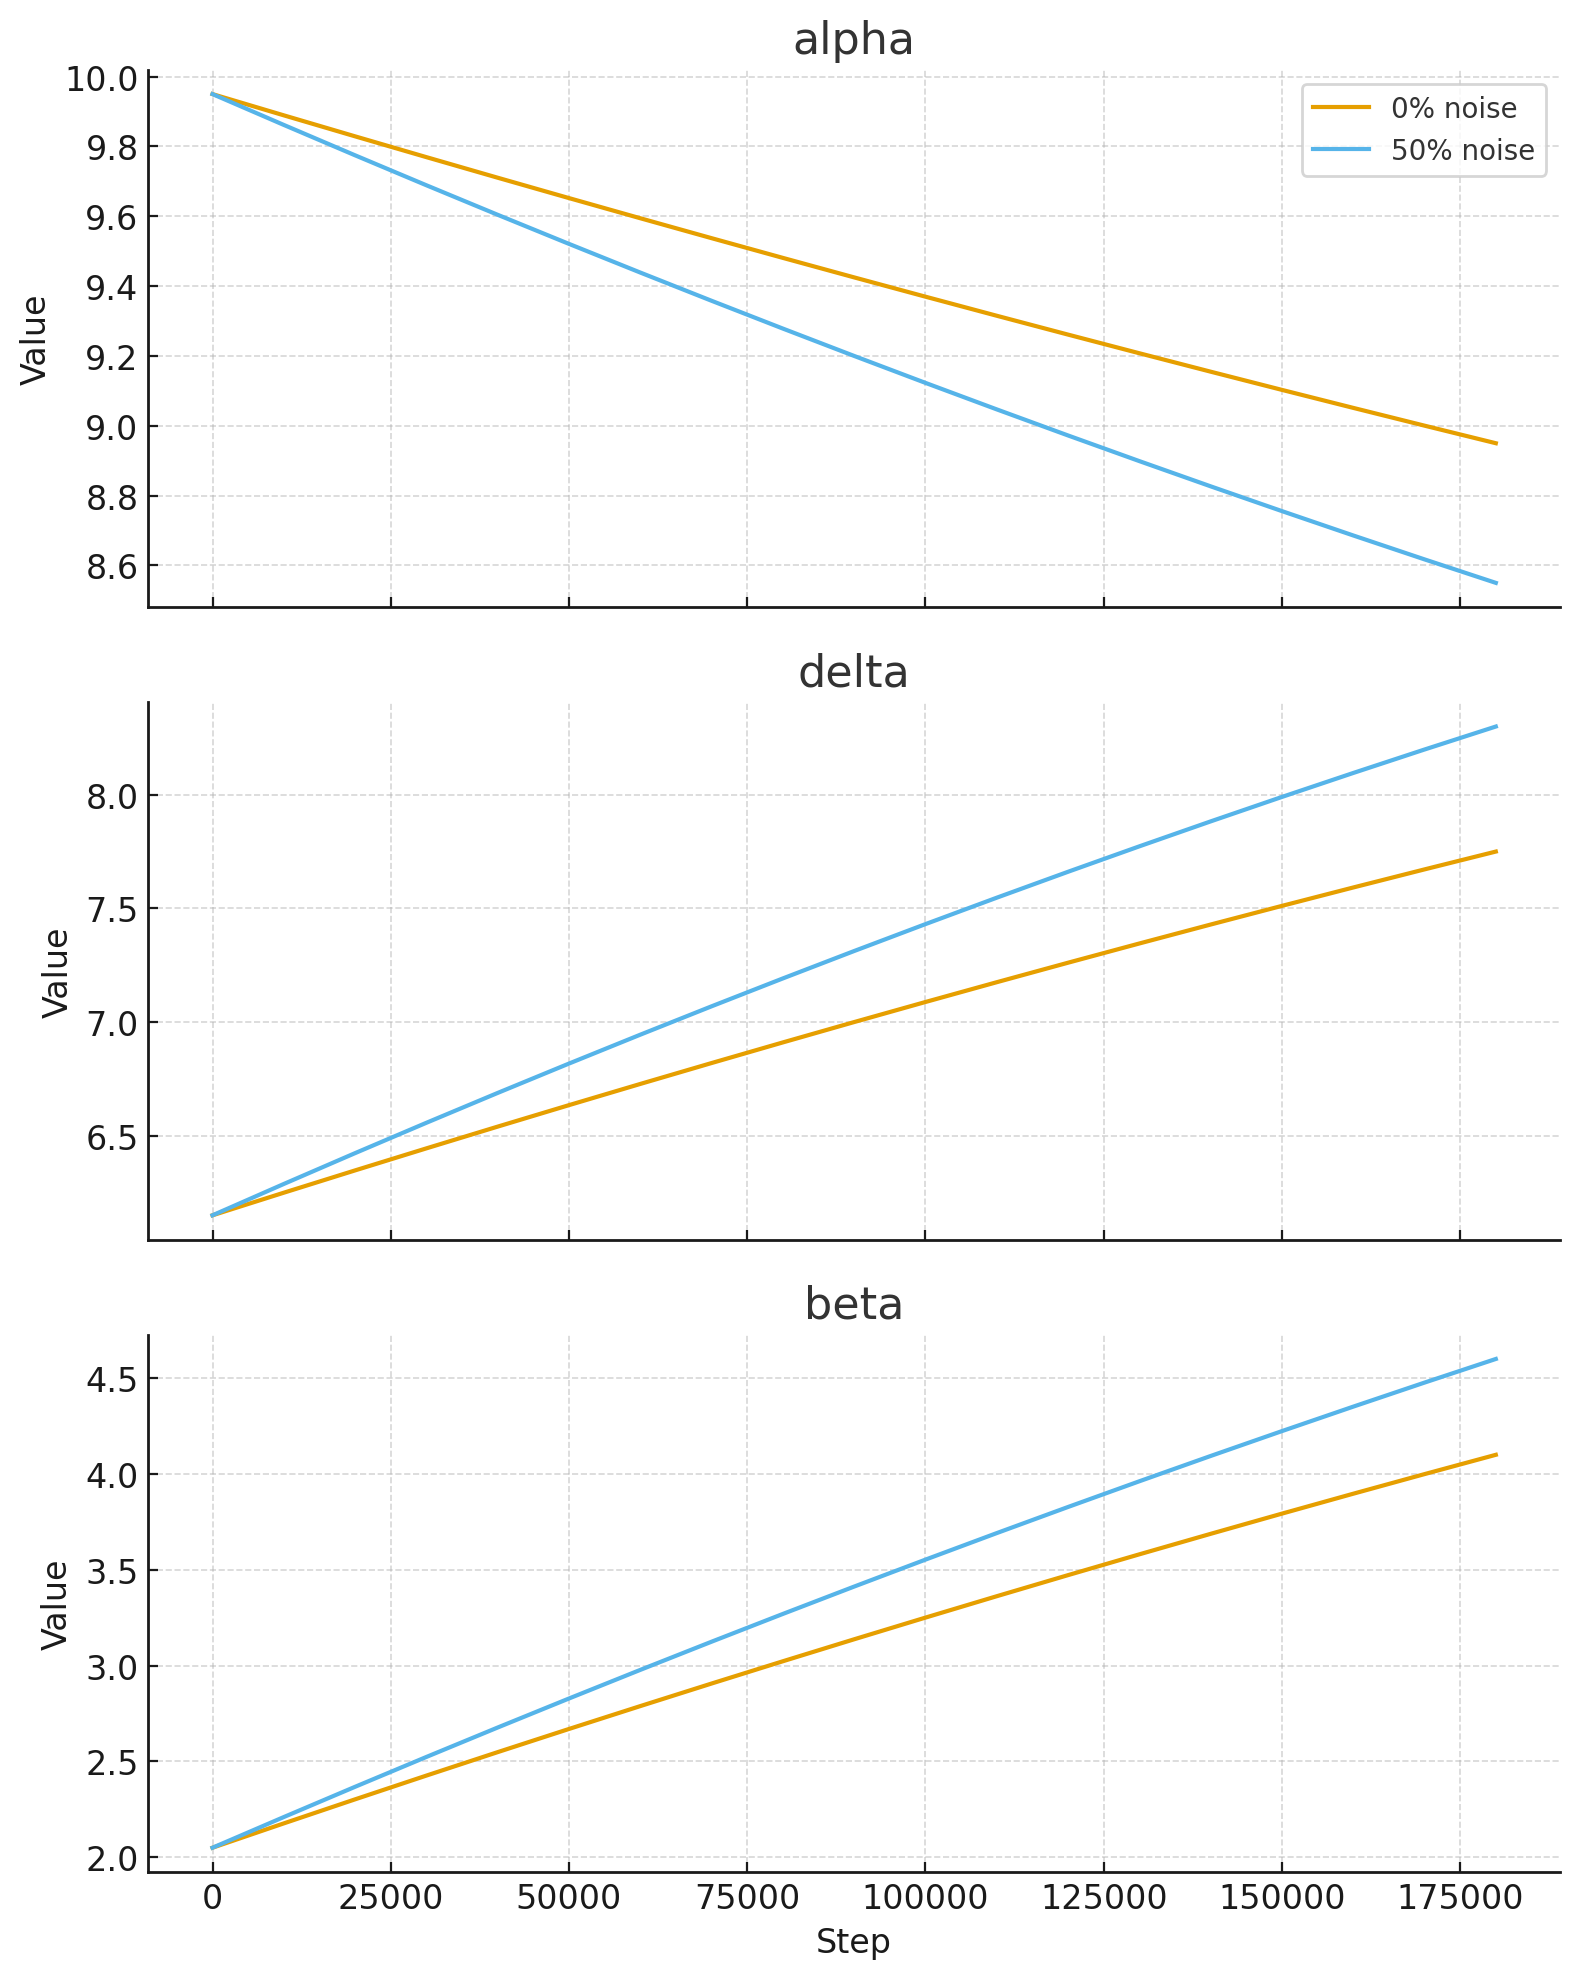
\includegraphics[scale=0.38]{abd.png}
    \caption{Plots showing how $\alpha,\beta,\delta$ change during training with 0\% symmetric noise and 50\% symmetric noise on CIFAR-100-M.}
    \label{fig:abd}
\end{figure}

\subsection{Time complexity analysis}
\label{supp:timecomplexity}

Without LiLAW, the runtime for each batch in each epoch in Algorithm~\ref{algo} is $O(|\theta| \cdot B)$ for the forward pass, loss calculation, backward pass, and update step, where $\theta$ are the model parameters and $B$ is the batch size. Going through all batches, we traverse the full dataset, so the runtime for each epoch is $O(|\theta| \cdot |\mathcal{D}_{t} + \mathcal{D}_{v}|)$. The total for $n$ epochs is $O(n \cdot |\theta| \cdot |\mathcal{D}_{t} + \mathcal{D}_{v}|)$.

With LiLAW, the runtime for the forward pass, loss calculation, backward pass, and update step is $O((|\theta| + 3) \cdot B) = O(|\theta| \cdot B)$ for each batch in each epoch in Algorithm~\ref{algo}, where $\theta$ are the model parameters, $B$ is the batch size (assuming the same batch size for training and validation), and 3 refers to the three LiLAW parameters. Going through all training batches and a single validation batch after each training batch, we have $O(|\theta| \cdot (|\mathcal{D}_{t} + \mathcal{D}_{v}| \cdot B)) = O(|\theta| \cdot|\mathcal{D}_{t} + \mathcal{D}_{v}|)$ as the runtime for each epoch. The total for $n$ epochs is $O(n \cdot |\theta| \cdot |\mathcal{D}_{t} + \mathcal{D}_{v}|)$, same as without LiLAW. We confirm empirically that across several runs of ViT-Base-16-224 with ImageNet-21K pretraining, on 224$\times$224 inputs with CIFAR-100-M trained for 10 epochs with batch size 16 with linear probing on the last two layers, we take about 45 minutes with or without LiLAW using one NVIDIA L40S GPU.

\subsection{Space complexity analysis}
\label{supp:spacecomplexity}

Without LiLAW, the space complexity for Algorithm~\ref{algo} is $O(|\theta|)$ for the model parameters $\theta$, $O(|\theta|)$ for the model parameter gradients, and $O(|\theta| \cdot B)$ for the activations during the forward pass, where $B$ is the batch size. The total is $O(|\theta| \cdot B)$.

With LiLAW, the space complexity for Algorithm~\ref{algo} is $O(|\theta| + 3) = O(|\theta|)$ for the model parameters, $\theta$, and the three LiLAW parameters, $\alpha, \beta, \delta$, $O(|\theta| + 3) = O(|\theta|)$ for the model parameter gradients and the LiLAW parameter gradients, and $O((|\theta| + 3) \cdot B) = O(|\theta| \cdot B)$ for the activations during the forward pass, where $B$ is the batch size (assuming the same batch size for training and validation). The total is $O(|\theta| \cdot B)$, same as without LiLAW.

\subsection{Extension of LiLAW to multi-label classification}
\label{sec:multilabel}
In the $c$-class multi-label classification case, we extend LiLAW as follows.

Let $\mathcal{D}_{t} = \{(x_i, \widetilde{y_i})\}^N_{i=1}$ represent the training set and $\mathcal{D}_{v} = \{(x_j, \widetilde{y_j})\}^{N+M}_{j=N+1}$ represent the validation set. As before, note that $(x_i, \widetilde{y_i})$ represents the pairs of inputs and observed (potentially synthetic/noisy) targets. For multi-label classification, $x_i \in \mathcal{X}$, where $\mathcal{X}$ is the input space and $\widetilde{y_i} \in \mathcal{Y} = \{0,1\}^c,$ is the output space with $c \in \mathbb{N}$ such that $c \ge 1$ is the total number of labels. Note that $\widetilde{y_i}[z]$ from $z \in \{0,...,c-1\}$ is 0 or 1 depending on whether the input has the observed label. Let $f_{\theta}: \mathcal{X} \rightarrow \mathcal{Y}$ be the neural network model, $\theta$ be its parameters, and $\sigma_i = \sigma(f_{\theta}(x_i))$ be the sigmoid of its logits. We keep a similar setup as before, except in $\mathcal{W}_\alpha$, $\mathcal{W}_\beta$, $\mathcal{W}_\delta$, we replace $s_i[\widetilde{y_i}]$ with $\frac{1}{k}\sum_i \sigma_i[\widetilde{y_i}]$ and $\max(s_i)$ with $\frac{1}{k}\sum\max_k{\sigma_i}$, where $k=\sum_i \widetilde{y_i}$ (total number of observed labels in $x_i$) and $\max_k{\sigma_i}$ is the $k$ max values in $\sigma_i$.

Instead of considering a single predicted value as in the multi-class classification case, we compute the average predicted probability for all $k$ observed labels corresponding to each sample. To determine the hardness of a sample, we also replace the single maximum probability with the average of the top $k$ probabilities since multiple labels may be relevant to each sample. The rest of the method remains the same, but this extension ensures that LiLAW can effectively weigh samples for multi-label classification, where each sample can have multiple observed labels rather than just one.

\subsection{Extension of LiLAW to regression}
\label{sec:regression}
In the regression case, we extend LiLAW as follows:

Let $\mathcal{D}_{t} = \{(x_i, \widetilde{y_i})\}^N_{i=1}$ represent the training set and $\mathcal{D}_{v} = \{(x_j, \widetilde{y_j})\}^{N+M}_{j=N+1}$ represent the validation set. As before, note that $(x_i, \widetilde{y_i})$ represents the pairs of inputs and observed (potentially synthetic/noisy) targets. However, for regression, $x_i \in \mathcal{X}$, where $\mathcal{X}$ is the input space and $\widetilde{y_i} \in \mathcal{Y} = \mathbb{R},$ is the output space. Let $f_{\theta}: \mathcal{X} \rightarrow \mathcal{Y}$ be the neural network model, $\theta$ be its parameters, and $f_{\theta}(x_i)$ be its output. Also, let $R$ be the range of the true targets, which is usually well-established in any given regression problem. We keep the setup similar to before, except in $\mathcal{W}_\alpha$, $\mathcal{W}_\beta$, $\mathcal{W}_\delta$, we replace $\alpha \cdot s_i[\widetilde{y_i}] - \max(s_i)$ with $\frac{1}{R}\cdot (\alpha \cdot f_{\theta}(x_i) - \widetilde{y_i})$, replace $\beta \cdot s_i[\widetilde{y_i}] - \max(s_i)$ with $\frac{1}{R}\cdot (\beta \cdot f_{\theta}(x_i) - \widetilde{y_i})$, and replace $\delta \cdot s_i[\widetilde{y_i}] - \max(s_i)$ with $\frac{1}{R}\cdot (\delta \cdot f_{\theta}(x_i) - \widetilde{y_i})$.

In the regression case, each sample has a real-valued target, so unlike classification tasks where samples can be labeled as correct or incorrect, regression tasks measure how far the model's prediction deviates from the observed target. This deviation therefore becomes the basis for determining sample difficulty: the smaller the deviation, the easier the sample and vice-versa. Since continuous targets can span vast numerical ranges, we normalize the difference by dividing by $R$, to prevent very large or very small absolute target values from disproportionately influencing the LiLAW weighting.

\subsection{Comparison of the three versions of LiLAW}
\label{comparison}
We compare the three weight functions ($\mathcal{W}_\alpha,\mathcal{W}_\beta,\mathcal{W}_\delta$) for the multi-class classification, multi-label classification, and regression cases. Note that the corresponding baseline loss function also changes accordingly.
\subsubsection{Multi-class classification}
\begin{align}
    \mathcal{W}_\alpha (s_i, \widetilde{y_i}) = \sigma(\alpha \cdot s_i[\widetilde{y_i}] - \max(s_i))\\
    \mathcal{W}_\beta (s_i, \widetilde{y_i}) = \sigma(-(\beta \cdot s_i[\widetilde{y_i}] - \max(s_i)))\\
    \mathcal{W}_\delta (s_i, \widetilde{y_i}) = \exp\biggl(-\frac{(\delta \cdot s_i[\widetilde{y_i}] - \max(s_i))^2}{2}\biggr)
\end{align}
\subsubsection{Multi-label classification}
\begin{align}
    \mathcal{W}_\alpha (s_i, \widetilde{y_i}) = \sigma\biggl(\alpha \cdot \frac{1}{k}\sum_i \sigma_i[\widetilde{y_i}] - \frac{1}{k}\sum\max_k{\sigma_i}\biggr)\\
    \mathcal{W}_\beta (s_i, \widetilde{y_i}) = \sigma\biggl(-\biggl(\beta \cdot \frac{1}{k}\sum_i \sigma_i[\widetilde{y_i}] - \frac{1}{k}\sum\max_k{\sigma_i}\biggr)\biggr)\\
    \mathcal{W}_\delta (s_i, \widetilde{y_i}) = \exp\biggl(-\frac{(\delta \cdot \frac{1}{k}\sum_i \sigma_i[\widetilde{y_i}] - \frac{1}{k}\sum\max_k{\sigma_i})^2}{2}\biggr)
\end{align}
\subsubsection{Regression}
\begin{align}
    \mathcal{W}_\alpha (s_i, \widetilde{y_i}) = \sigma\biggl(\frac{1}{R}\cdot (\alpha \cdot f_{\theta}(x_i) - \widetilde{y_i})\biggr)\\
    \mathcal{W}_\beta (s_i, \widetilde{y_i}) = \sigma\biggl(-\biggl(\frac{1}{R}\cdot (\beta \cdot f_{\theta}(x_i) - \widetilde{y_i})\biggr)\biggr)\\
    \mathcal{W}_\delta (s_i, \widetilde{y_i}) = \sigma\biggl(-\biggl(\frac{1}{R}\cdot (\delta \cdot f_{\theta}(x_i) - \widetilde{y_i})\biggr)\biggr)
\end{align}

\subsection{Implementation Details for General Imaging and Medical Imaging Dataset}
\label{imp}

\begin{enumerate}[leftmargin=*,labelindent=0pt,label=\textbf{--}]
    \itemsep-0.2em
    \item ViT-Base-16-224~\citep{vit}, with ImageNet-21K pretraining, on 224$\times$224 inputs with CIFAR-100-M, CIFAR-10-M, FashionMNIST-M, and MNIST-M. We trained for 10 epochs with batch size 16, learning rate $0.0002$, and weight decay $0$, using a linear learning rate scheduler. 
    \item ResNet-18~\citep{resnet}, with ImageNet-21K pretraining, on 224$\times$224 inputs with the MedMNISTv2 datasets. We trained for 100 epochs with batch size 128, learning rate $0.0001$, and weight decay $0$, using a multi-step learning rate scheduler with a $0.1$ decay at 50 epochs and 75 epochs, as mentioned in~\citet{medmnistv2}.
\end{enumerate}
\vspace{-1em}
All of the above models use the Adam optimizer~\citep{kingma2014adam} with early stopping. We use a warmup period of 1 epoch to ensure that the model briefly learns from the data before using LiLAW. The parameters are initialized to $\alpha_{init}, \beta_{init}, \delta_{init} = 10, 2, 6$, with learning rates $\alpha_{lr}, \beta_{lr}, \delta_{lr} = 0.005$, and weight decays $\alpha_{wd}, \beta_{wd}, \delta_{wd} = 0.0001$ for manual gradient descent. Our method is not too sensitive to these choices. We mainly use cross-entropy loss, but also evaluate using focal loss in~\ref{supp:loss}.

%Additionally, the CIFAR-100-M, CIFAR-10-M, FashionMNIST-M, and MNIST-M experiments with ViT-Base-16-224, with ImageNet-21K pretraining, on 224x224 inputs were compared with: fine-tuning on the full pretrained model (without LiLAW) and fine-tuning solely on the last 2 layers of the pretrained model (with LiLAW).

\subsection{Performance with various noise levels}
\label{supp:noiselevel}

\begin{table}[h!] \centering  \begin{tabular}{cccc} \hline \textbf{Noise Level (\%)} & \textbf{Top-1 Acc. (\%)} & \textbf{Top-5 Acc. (\%)} & \textbf{AUROC} \\ \hline 0 & \hspace{0.5em}76.41 \textcolor{Green}{$\uparrow$} \hspace{0.5em}4.44 \textcolor{BrickRed}{$\downarrow$} 0.01\hspace{0.5em} & \hspace{0.5em}95.39 \textcolor{Green}{$\uparrow$} \hspace{0.5em}0.68 \textcolor{Green}{$\uparrow$} 0.16\hspace{0.5em} & 0.9926 \textcolor{BrickRed}{$\downarrow$} 0.0038 \textcolor{BrickRed}{$\downarrow$} 0.0005 \\ 10 & \hspace{0.5em}75.45 \textcolor{Green}{$\uparrow$} \hspace{0.5em}4.14 \textcolor{Green}{$\uparrow$} 0.20\hspace{0.5em} & \hspace{0.5em}94.62 \textcolor{Green}{$\uparrow$} \hspace{0.5em}0.70 \textcolor{Green}{$\uparrow$} 0.14\hspace{0.5em} & 0.9910 \textcolor{BrickRed}{$\downarrow$} 0.0050 \textcolor{BrickRed}{$\downarrow$} 0.0002 \\ 20 & \hspace{0.5em}74.54 \textcolor{Green}{$\uparrow$} \hspace{0.5em}4.18 \textcolor{Green}{$\uparrow$} 0.66\hspace{0.5em} & \hspace{0.5em}93.48 \textcolor{Green}{$\uparrow$} \hspace{0.5em}1.32 \textcolor{Green}{$\uparrow$} 0.23\hspace{0.5em} & 0.9867 \textcolor{Green}{$\uparrow$} 0.0003 \textcolor{Green}{$\uparrow$} 0.0001 \\ 30 & \hspace{0.5em}68.97 \textcolor{Green}{$\uparrow$} \hspace{0.5em}8.89 \textcolor{Green}{$\uparrow$} 0.74\hspace{0.5em} & \hspace{0.5em}91.11 \textcolor{Green}{$\uparrow$} \hspace{0.5em}3.18 \textcolor{Green}{$\uparrow$} 0.30\hspace{0.5em} & 0.9821 \textcolor{Green}{$\uparrow$} 0.0012 \textcolor{Green}{$\uparrow$} 0.0006 \\ 40 & 64.25 \textcolor{Green}{$\uparrow$} 12.52 \textcolor{Green}{$\uparrow$} 0.88 & \hspace{0.5em}88.15 \textcolor{Green}{$\uparrow$} \hspace{0.5em}5.40 \textcolor{Green}{$\uparrow$} 0.49\hspace{0.5em} & 0.9748 \textcolor{Green}{$\uparrow$} 0.0087 \textcolor{Green}{$\uparrow$} 0.0010 \\ 50 & 58.03 \textcolor{Green}{$\uparrow$} 17.17 \textcolor{Green}{$\uparrow$} 1.35 & \hspace{0.5em}85.42 \textcolor{Green}{$\uparrow$} \hspace{0.5em}7.19 \textcolor{Green}{$\uparrow$} 0.67\hspace{0.5em} & 0.9706 \textcolor{Green}{$\uparrow$} 0.0105 \textcolor{Green}{$\uparrow$} 0.0013 \\ 60 & 52.32 \textcolor{Green}{$\uparrow$} 21.30 \textcolor{Green}{$\uparrow$} 1.80 & 80.38 \textcolor{Green}{$\uparrow$} 10.84 \textcolor{Green}{$\uparrow$} 1.10 & 0.9588 \textcolor{Green}{$\uparrow$} 0.0183 \textcolor{Green}{$\uparrow$} 0.0022 \\ 70 & 13.87 \textcolor{Green}{$\uparrow$} 56.96 \textcolor{Green}{$\uparrow$} 2.63 & 37.87 \textcolor{Green}{$\uparrow$} 51.11 \textcolor{Green}{$\uparrow$} 1.39 & 0.8335 \textcolor{Green}{$\uparrow$} 0.1378 \textcolor{Green}{$\uparrow$} 0.0033 \\ 80 & \hspace{0.5em}7.78 \textcolor{Green}{$\uparrow$} 58.86 \textcolor{Green}{$\uparrow$} 3.20 & 25.45 \textcolor{Green}{$\uparrow$} 59.92 \textcolor{Green}{$\uparrow$} 1.93 & 0.7509 \textcolor{Green}{$\uparrow$} 0.2082 \textcolor{Green}{$\uparrow$} 0.0052 \\ 90 & \hspace{0.5em}1.48 \textcolor{Green}{$\uparrow$} 51.55 \textcolor{Green}{$\uparrow$} 2.66 & 6.96\hspace{0.5em} \textcolor{Green}{$\uparrow$} 66.58 \textcolor{Green}{$\uparrow$} 1.74 & 0.5952 \textcolor{Green}{$\uparrow$} 0.3268 \textcolor{Green}{$\uparrow$} 0.0036 \\ \hline \end{tabular} \caption{Results with different levels of symmetric noise on CIFAR-100-M. \label{table:noiselevels}} \vspace{-1em}\end{table}

In Table~\ref{table:noiselevels}, we report test performance across noise levels from 0\% to 90\% in increments of 10\%. At every setting, LiLAW consistently improves both accuracy and AUROC over the baseline. Notably, linear probing with LiLAW, top-1 accuracy under up to 50\% noise matches that of noiseless full fine-tuning.
\newpage

\subsection{Ablation study on $\alpha,\beta,\delta$}
\label{supp:ablation}

\begin{table*}[!htb] \centering \begin{tabular}{lccccc} \hline \textbf{Parameters Used} & \textbf{Noise Level (\%)} & \textbf{Top-1 Acc. (\%)} & \textbf{Top-5 Acc. (\%)} & \textbf{AUROC} \\ \hline \multirow{2}{*}{$\alpha, \beta, \delta$} & 0 & \hspace{0.5em}76.41 \textcolor{Green}{$\uparrow$} \hspace{0.5em}4.44 \textcolor{BrickRed}{$\downarrow$} 0.10\hspace{0.5em} & 95.39 \textcolor{Green}{$\uparrow$} 0.68 \textcolor{Green}{$\uparrow$} 0.00 & 0.9926 \textcolor{BrickRed}{$\downarrow$} 0.0038  \textcolor{BrickRed}{$\downarrow$} 0.0011 \\ & 50 & 58.03 \textcolor{Green}{$\uparrow$} 17.17 \textcolor{Green}{$\uparrow$} 1.36 & 85.42 \textcolor{Green}{$\uparrow$} 7.19 \textcolor{Green}{$\uparrow$} 0.67 & 0.9706 \textcolor{Green}{$\uparrow$} 0.0105 \textcolor{Green}{$\uparrow$} 0.0013 \\ \hline \multirow{2}{*}{$\alpha, \beta$} & 0 & \hspace{0.5em}76.41 \textcolor{Green}{$\uparrow$} \hspace{0.5em}4.44 \textcolor{Green}{$\uparrow$} 0.07\hspace{0.5em} & 95.39 \textcolor{Green}{$\uparrow$} 0.68  \textcolor{Green}{$\uparrow$} 0.06 & 0.9926 \textcolor{BrickRed}{$\downarrow$} 0.0038  \textcolor{BrickRed}{$\downarrow$} 0.0002 \\ & 50 & 58.03 \textcolor{Green}{$\uparrow$} 17.17  \textcolor{Green}{$\uparrow$} 0.35 & 85.42 \textcolor{Green}{$\uparrow$} 7.19 \textcolor{Green}{$\uparrow$} 0.07 & 0.9706 \textcolor{Green}{$\uparrow$} 0.0105 \textcolor{Green}{$\uparrow$} 0.0001 \\ \hline \multirow{2}{*}{$\alpha, \delta$} & 0 & \hspace{0.5em}76.41 \textcolor{Green}{$\uparrow$} \hspace{0.5em}4.44 \textcolor{Green}{$\uparrow$} 0.01\hspace{0.5em} & 95.39 \textcolor{Green}{$\uparrow$} 0.68 \textcolor{BrickRed}{$\downarrow$} 0.01 & 0.9926 \textcolor{BrickRed}{$\downarrow$} 0.0038  \textcolor{BrickRed}{$\downarrow$} 0.0008 \\ & 50 & 58.03 \textcolor{Green}{$\uparrow$} 17.17  \textcolor{BrickRed}{$\downarrow$} 0.69 & 85.42 \textcolor{Green}{$\uparrow$} 7.19 \textcolor{BrickRed}{$\downarrow$} 0.31 & 0.9706 \textcolor{Green}{$\uparrow$} 0.0105 \textcolor{BrickRed}{$\downarrow$} 0.0012 \\ \hline \multirow{2}{*}{$\beta, \delta$} & 0 & \hspace{0.5em}76.41 \textcolor{Green}{$\uparrow$} \hspace{0.5em}4.44 \textcolor{BrickRed}{$\downarrow$} 1.59\hspace{0.5em} & 95.39 \textcolor{Green}{$\uparrow$} 0.68 \textcolor{BrickRed}{$\downarrow$} 0.29 & 0.9926 \textcolor{BrickRed}{$\downarrow$} 0.0038  \textcolor{BrickRed}{$\downarrow$} 0.0023 \\ & 50 & 58.03 \textcolor{Green}{$\uparrow$} 17.17 \textcolor{BrickRed}{$\downarrow$} 0.14 & 85.42 \textcolor{Green}{$\uparrow$} 7.19 \textcolor{Green}{$\uparrow$} 0.35 & 0.9706 \textcolor{Green}{$\uparrow$} 0.0105 \textcolor{Green}{$\uparrow$} 0.0005 \\ \hline \multirow{2}{*}{$\alpha$} & 0 & \hspace{0.5em}76.41 \textcolor{Green}{$\uparrow$} \hspace{0.5em}4.44 \textcolor{BrickRed}{$\downarrow$} 1.10 \hspace{0.5em} & 95.39 \textcolor{Green}{$\uparrow$} 0.68  \textcolor{Green}{$\uparrow$} 0.05 & 0.9926 \textcolor{BrickRed}{$\downarrow$} 0.0038  \textcolor{BrickRed}{$\downarrow$} 0.0001 \\ & 50 & 58.03 \textcolor{Green}{$\uparrow$} 17.17 \textcolor{BrickRed}{$\downarrow$} 0.69 & 85.42 \textcolor{Green}{$\uparrow$} 7.19 \textcolor{BrickRed}{$\downarrow$} 0.30 & 0.9706 \textcolor{Green}{$\uparrow$} 0.0105 \textcolor{BrickRed}{$\downarrow$} 0.0007 \\ \hline \multirow{2}{*}{$\beta$} & 0 & \hspace{0.5em}76.41 \textcolor{Green}{$\uparrow$} \hspace{0.5em}4.44 \textcolor{BrickRed}{$\downarrow$} 1.23\hspace{0.5em} & 95.39 \textcolor{Green}{$\uparrow$} 0.68 \textcolor{BrickRed}{$\downarrow$} 0.21 & 0.9926 \textcolor{BrickRed}{$\downarrow$} 0.0038  \textcolor{BrickRed}{$\downarrow$} 0.0011 \\ & 50 & 58.03 \textcolor{Green}{$\uparrow$} 17.17  \textcolor{BrickRed}{$\downarrow$} 0.69 & 85.42 \textcolor{Green}{$\uparrow$} 7.19 \textcolor{BrickRed}{$\downarrow$} 0.31 & 0.9706 \textcolor{Green}{$\uparrow$} 0.0105 \textcolor{BrickRed}{$\downarrow$} 0.0007 \\ \hline \multirow{2}{*}{$\delta$} & 0 & \hspace{0.5em}76.41 \textcolor{Green}{$\uparrow$} \hspace{0.5em}4.44 \textcolor{BrickRed}{$\downarrow$} 1.90 \hspace{0.5em} & 95.39 \textcolor{Green}{$\uparrow$} 0.68 \textcolor{BrickRed}{$\downarrow$} 0.26 & 0.9926 \textcolor{BrickRed}{$\downarrow$} 0.0038  \textcolor{BrickRed}{$\downarrow$} 0.0026 \\ & 50 & 58.03 \textcolor{Green}{$\uparrow$} 17.17  \textcolor{BrickRed}{$\downarrow$} 0.68 & 85.42 \textcolor{Green}{$\uparrow$} 7.19 \textcolor{BrickRed}{$\downarrow$} 0.30 & 0.9706 \textcolor{Green}{$\uparrow$} 0.0105 \textcolor{BrickRed}{$\downarrow$} 0.0007 \\ \hline \end{tabular} \caption{Results of ablating the parameters with different levels of symmetric noise on CIFAR-100-M. \label{table:ablation}} \end{table*}
\vspace{-1em}
In Table \ref{table:ablation}, we present an ablation study examining the impact of different combinations of the LiLAW parameters ($ \alpha,\beta,\delta$) on model performance under varying noise levels. Using all three parameters yields the highest performance gains, which are especially significant at higher noise levels. This demonstrates the full potential of LiLAW in improving model robustness and accuracy. Excluding two of the weights results in very poor performance. Including two of the weights occasionally results in minor improvements in performance, however including all three yields the best results.
\vspace{-0.5em}
\subsection{Performance with and without calibration}
\label{supp:calibration}

\begin{table*}[h!] \centering { \begin{tabular}{l|cccc} \hline \textbf{Calibration} & \textbf{Noise Level (\%)} & \textbf{Top-1 Acc. (\%)} & \textbf{Top-5 Acc. (\%)} & \textbf{AUROC} \\ \hline \multirow{2}{*}{Without calibration} & 0 & \hspace{0.5em}76.41 \textcolor{Green}{$\uparrow$} \hspace{0.5em}4.44 \textcolor{BrickRed}{$\downarrow$} 0.01\hspace{0.5em} & \hspace{0.5em}95.39 \textcolor{Green}{$\uparrow$} 0.68 \textcolor{Green}{$\uparrow$} 0.16\hspace{0.5em} & 0.9926 \textcolor{BrickRed}{$\downarrow$} 0.0038 \textcolor{BrickRed}{$\downarrow$} 0.0005 \\ & 50 & 58.03 \textcolor{Green}{$\uparrow$} 17.17 \textcolor{Green}{$\uparrow$} 1.35 & \hspace{0.5em}85.42 \textcolor{Green}{$\uparrow$} 7.19 \textcolor{Green}{$\uparrow$} 0.67\hspace{0.5em} & 0.9706 \textcolor{Green}{$\uparrow$} 0.0105 \textcolor{Green}{$\uparrow$} 0.0013 \\ \hline \multirow{2}{*}{With calibration} & 0 & 76.24 \textcolor{Green}{$\uparrow$} \hspace{0.5em}3.79 \textcolor{BrickRed}{$\downarrow$} 0.01 & 95.34 \textcolor{Green}{$\uparrow$} 0.11 \textcolor{Green}{$\uparrow$} 0.07 & 0.9923 \textcolor{Green}{$\uparrow$} 0.0044 \textcolor{BrickRed}{$\downarrow$} 0.0001 \\ & 50 & 58.43 \textcolor{Green}{$\uparrow$} 16.77 \textcolor{Green}{$\uparrow$} 1.32 & 84.32 \textcolor{Green}{$\uparrow$} 8.29 \textcolor{Green}{$\uparrow$} 0.67 & 0.9715 \textcolor{Green}{$\uparrow$} 0.0112 \textcolor{Green}{$\uparrow$} 0.0013 \\ \hline \end{tabular}} \caption{Results with and without calibration with different levels of symmetric noise on CIFAR-100-M.\label{table:calibration}} \end{table*}
\vspace{-0.5em}
According to Table \ref{table:calibration}, with and without noise, applying LiLAW leads to significant performance gains, regardless of calibration. When calibration is combined with LiLAW, it works synergistically to enhance robustness to noise. The performance boost at 50\% noise indicates that LiLAW effectively mitigates the effects of label noise. Using LiLAW with 50\% noise surpasses the top-1 accuracy of not using LiLAW with 0\% noise. We note that there is a reasonable boost in test accuracy when using LiLAW even when there is 0\% noise since we are pushing unconfident predictions to be more confident. There is a slight decrease in AUROC in nearly all cases where there is 0\% noise since the model may need to be slightly less confident on the thresholds to improve accuracy.

\subsection{Performance with and without a clean validation set}
\label{supp:cleanvalset}

In Table \ref{table:cleanval}, we show test performance with and without a clean validation set. We see that LiLAW enhances performance even without a clean validation set, demonstrating its robustness in practical scenarios where obtaining a clean validation set may be challenging. The improvements with a clean validation set are comparable to those without one, indicating that LiLAW does not heavily rely on validation set cleanliness and can easily adapt to noisy validation data. In addition, training on only 50\% of the data that is clean (without using the 50\% noisy data) achieves worse performance than using LiLAW without a clean validation set, further supporting our claim that LiLAW is robust to noise and more effective than pruning.

\begin{table*}[h!] \centering \resizebox{\textwidth}{!}{ \begin{tabular}{l|cccc} \hline \textbf{Validation set cleanliness} & \textbf{Noise Level (\%)} & \textbf{Top-1 Acc. (\%)} & \textbf{Top-5 Acc. (\%)} & \textbf{AUROC} \\ \hline \multirow{2}{*}{Without a clean validation set} & 0 & \hspace{0.5em}76.41 \textcolor{Green}{$\uparrow$} \hspace{0.5em}4.44 \textcolor{BrickRed}{$\downarrow$} 0.01\hspace{0.5em} & \hspace{0.5em}95.39 \textcolor{Green}{$\uparrow$} 0.68 \textcolor{Green}{$\uparrow$} 0.16\hspace{0.5em} & 0.9926 \textcolor{BrickRed}{$\downarrow$} 0.0038 \textcolor{BrickRed}{$\downarrow$} 0.0005 \\ & 50 & 58.03 \textcolor{Green}{$\uparrow$} 17.17 \textcolor{Green}{$\uparrow$} 1.35 & \hspace{0.5em}85.42 \textcolor{Green}{$\uparrow$} 7.19 \textcolor{Green}{$\uparrow$} 0.67\hspace{0.5em} & 0.9706 \textcolor{Green}{$\uparrow$} 0.0105 \textcolor{Green}{$\uparrow$} 0.0013 \\ \hline \multirow{2}{*}{With a clean validation set} & 0 & 77.40 \textcolor{Green}{$\uparrow$} \hspace{0.5em}2.63 \textcolor{Green}{$\uparrow$} 0.01 & 95.56 \textcolor{Green}{$\uparrow$} 0.11 \textcolor{BrickRed}{$\downarrow$} 0.07 & 0.9934 \textcolor{BrickRed}{$\downarrow$} 0.0052 \textcolor{BrickRed}{$\downarrow$} 0.0001 \\ & 50 & 55.42 \textcolor{Green}{$\uparrow$} 19.78 \textcolor{Green}{$\uparrow$} 1.29 & 84.72 \textcolor{Green}{$\uparrow$} 7.89 \textcolor{Green}{$\uparrow$} 0.70 & 0.9734 \textcolor{Green}{$\uparrow$} 0.0077 \textcolor{Green}{$\uparrow$} 0.0013 \\ \hline Trained on 50\% of data that is clean & 0 & 74.34 & 94.94 & 0.9919 \\ \hline \end{tabular}} \caption{Results with and without a clean validation set on CIFAR-100-M with 50\% symmetric noise. We also compare these results to when the model is trained only on the 50\% of the data that is clean. \label{table:cleanval}} \end{table*}

\subsection{Performance under different random seeds}
\label{supp:randseed}

Table~\ref{table:seeds} shows that the improvements observed with LiLAW are consistent across five different random initializations and choices of meta-validation sets, as reflected by the low standard deviations over five independent runs. Under 0\% noise and 50\% noise, LiLAW not only achieves much higher accuracy but also reduces variability across the runs. This demonstrates that LiLAW yields reliable performance improvements across various training conditions, highlighting its robustness to noise and stochasticity. 

Using LiLAW without linear probing also leads to a boost from full-training without LiLAW, however, performance becomes very stable as can be seen with very low standard deviations. To allow the model to not only be robust to noise, but correct some of it, LiLAW needs to be used in conjunction with linear probing.

\begin{table}[h!]
\centering
\begin{tabular}{cccccc}
\hline
\textbf{Noise Level (\%)} & \textbf{LiLAW} & \textbf{Top-1 Acc. (\%)} & \textbf{Top-5 Acc. (\%)} & \textbf{AUROC} \\
\hline
\multirow{2}{*}{0}  & {\color{BrickRed}\texttimes} (full fine-tuning) & 74.93 $\pm$ 1.07 & 94.56 $\pm$ 0.51 & 0.9918 $\pm$ 0.0009 \\
& {\color{BrickRed}\texttimes} (linear probing) & 81.01 $\pm$ 0.15 & 94.84 $\pm$ 0.10 & 0.9887 $\pm$ 0.0003 \\
  & {\color{Green}\checkmark} (linear probing) & 80.87 $\pm$ 0.27 & 95.91 $\pm$ 0.08 & 0.9881 $\pm$ 0.0003 \\ \hline
\multirow{2}{*}{50} & {\color{BrickRed}\texttimes} (full fine-tuning) & 46.32 $\pm$ 7.82 & 76.12 $\pm$ 5.98 & 0.9537 $\pm$ 0.0142 \\
& {\color{BrickRed}\texttimes} (linear probing) & 75.00 $\pm$ 0.42 & 92.31 $\pm$ 0.28 & 0.9822 $\pm$ 0.0036 \\
 & {\color{Green}\checkmark} (linear probing) & 75.68 $\pm$ 1.03 & 92.91 $\pm$ 0.53 & 0.9820 $\pm$ 0.0012 \\
\hline
\end{tabular}
\caption{Performance (mean $\pm$ std over 5 runs with different random seeds) on CIFAR-100-M across different noise levels with (\color{Green}{\checkmark}\color{Black}) and without (\color{BrickRed}{\texttimes}\color{Black}) LiLAW.}
\label{table:seeds}
\end{table}

\iffalse
\begin{figure}[h!]
    \centering
    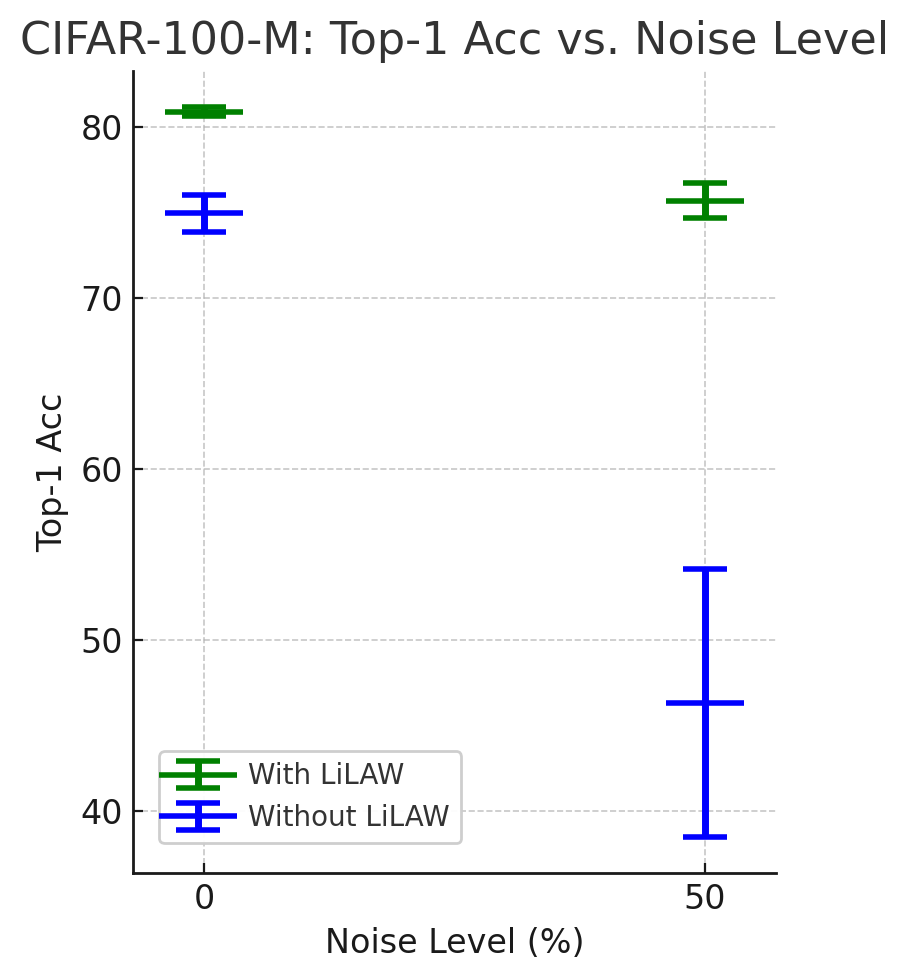
\includegraphics[scale=0.38]{top1vnoise.png}
    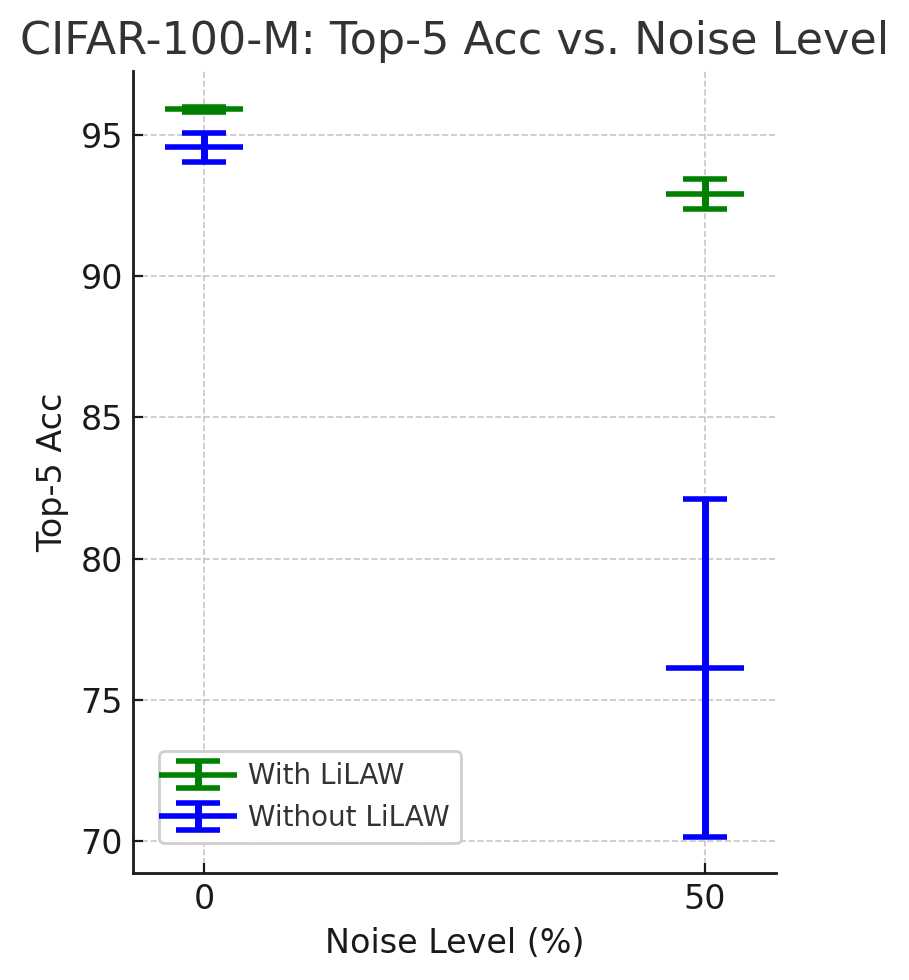
\includegraphics[scale=0.38]{top5vnoise.png}
    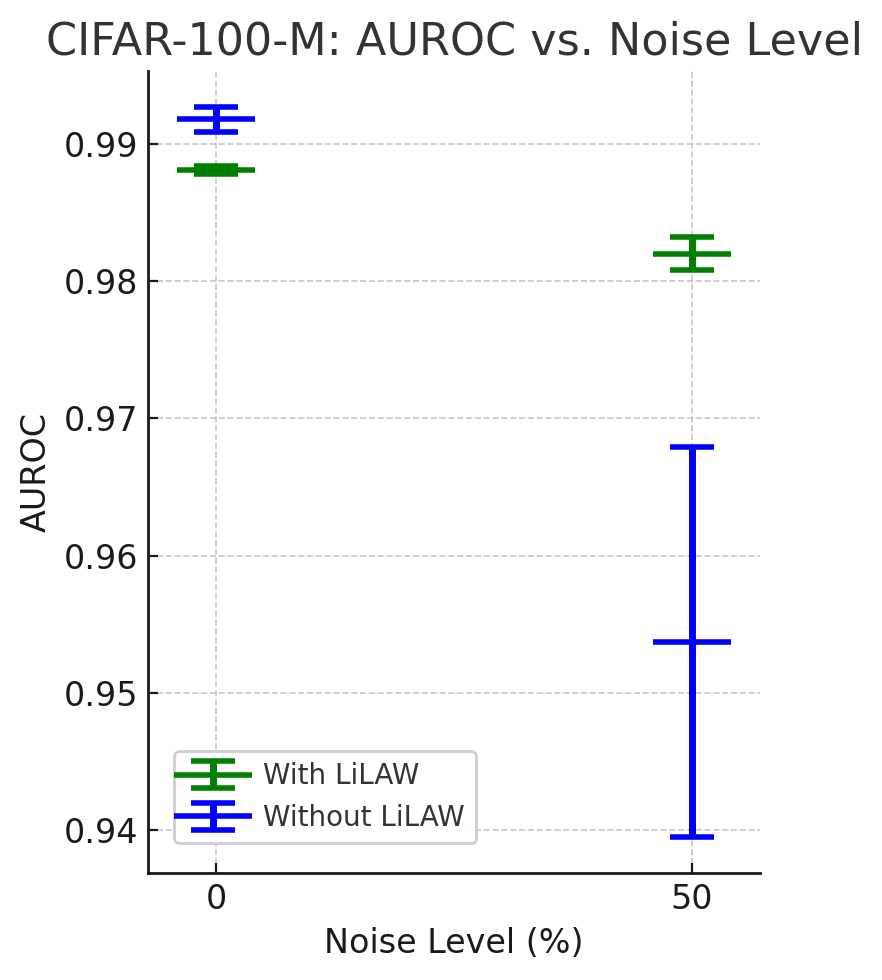
\includegraphics[scale=0.38]{aurocvnoise.png}
    \caption{Plots with means and standard deviations of top-1 accuracy, top-5 accuracy, and AUROC across 5 runs with different random seeds on CIFAR-100-M under different noise levels.}
    \label{fig:seeds}
\end{figure}
\fi
\subsection{Performance under different loss functions}
\label{supp:loss}

In Table \ref{table:losses}, we see that LiLAW provides performance gains with both cross-entropy and focal loss functions, indicating its versatility even when we use different loss landscapes that are already designed to handle issues such as class imbalance. Although noisy labels can negatively affect training with either of these two losses, LiLAW's adaptive weighting helps mitigate the impact of mislabeled or noisy data by dynamically adjusting the loss weight of each sample. Note that the boosts with LiLAW with cross-entropy loss and with focal loss reach similar accuracies.

\begin{table*}[h!] \centering \resizebox{\textwidth}{!}{ \begin{tabular}{lccccc} \hline \textbf{Loss Function} & \textbf{Noise Level (\%)} & \textbf{Top-1 Acc. (\%)} & \textbf{Top-5 Acc. (\%)} & \textbf{AUROC} \\ \hline \multirow{2}{*}{Cross-Entropy} & 0 & \hspace{0.5em}76.41 \textcolor{Green}{$\uparrow$} \hspace{0.5em}4.44 \textcolor{BrickRed}{$\downarrow$} 0.01\hspace{0.5em} & \hspace{0.5em}95.39 \textcolor{Green}{$\uparrow$} 0.68 \textcolor{Green}{$\uparrow$} 0.16\hspace{0.5em} & 0.9926 \textcolor{BrickRed}{$\downarrow$} 0.0038 \textcolor{BrickRed}{$\downarrow$} 0.0005 \\ & 50 & 58.03 \textcolor{Green}{$\uparrow$} 17.17 \textcolor{Green}{$\uparrow$} 1.35 & \hspace{0.5em}85.42 \textcolor{Green}{$\uparrow$} 7.19 \textcolor{Green}{$\uparrow$} 0.67\hspace{0.5em} & 0.9706 \textcolor{Green}{$\uparrow$} 0.0105 \textcolor{Green}{$\uparrow$} 0.0013 \\ \hline \multirow{2}{*}{Focal Loss~\citep{focalloss}} & 0 & 78.51 \textcolor{Green}{$\uparrow$} \hspace{0.5em}1.63 \textcolor{BrickRed}{$\downarrow$} 0.18 & 96.70 \textcolor{Green}{$\uparrow$} 0.84 \textcolor{BrickRed}{$\downarrow$} 0.06 & 0.9940 \textcolor{Green}{$\uparrow$} 0.0065 \textcolor{BrickRed}{$\downarrow$} 0.0001 \\ & 50 & 56.66 \textcolor{Green}{$\uparrow$} 18.61 \textcolor{Green}{$\uparrow$} 1.15 & 85.36 \textcolor{Green}{$\uparrow$} 7.34 \textcolor{Green}{$\uparrow$} 0.62 & 0.9746 \textcolor{Green}{$\uparrow$} 0.0047 \textcolor{Green}{$\uparrow$} 0.0014 \\ \hline \end{tabular}} \caption{Results of two loss functions with varying levels of symmetric noise on CIFAR-100-M. \label{table:losses}} \end{table*}

\subsection{Effect of validation set size}
\label{supp:valsize}

In Table \ref{table:valsize}, we analyze the effect of varying the validation set size (as a percentage of the training set size) on the test performance. We see that we do not need too much validation data to obtain high performance using LiLAW. Note that we only use one random batch from the validation set. We see that a 15\% validation set size strikes a good balance between having enough validation data for LiLAW while leaving sufficient data for model training. Simply increasing the validation set size does not guarantee better performance. As a result, we conclude that there is minor variability in the boost from LiLAW depending on the validation set size, but LiLAW consistently improves accuracy across all validation set sizes, demonstrating its robustness in noisy settings.

\begin{table}[h!] \centering  \begin{tabular}{cccc} \hline \textbf{Validation Set Size (\%)} & \textbf{Top-1 Acc. (\%)} & \textbf{Top-5 Acc. (\%)} & \textbf{AUROC} \\ \hline 5 & 47.43 \textcolor{Green}{$\uparrow$} 28.40 \textcolor{Green}{$\uparrow$} 1.13 & 76.95 \textcolor{Green}{$\uparrow$} 15.75 \textcolor{Green}{$\uparrow$} 0.59 & 0.9513 \textcolor{Green}{$\uparrow$} 0.0300 \textcolor{Green}{$\uparrow$} 0.0012 \\ 10 & 42.58 \textcolor{Green}{$\uparrow$} 32.62 \textcolor{Green}{$\uparrow$} 1.62 & 72.63 \textcolor{Green}{$\uparrow$} 19.66 \textcolor{Green}{$\uparrow$} 1.03 & 0.9445 \textcolor{Green}{$\uparrow$} 0.0359 \textcolor{Green}{$\uparrow$} 0.0015 \\ 15 & 58.03 \textcolor{Green}{$\uparrow$} 17.17 \textcolor{Green}{$\uparrow$} 1.35 & \hspace{0.5em}85.42 \textcolor{Green}{$\uparrow$} \hspace{0.5em}7.19 \textcolor{Green}{$\uparrow$} 0.67\hspace{0.5em} & 0.9706 \textcolor{Green}{$\uparrow$} 0.0105 \textcolor{Green}{$\uparrow$} 0.0013 \\ 20 & 38.21 \textcolor{Green}{$\uparrow$} 36.89 \textcolor{Green}{$\uparrow$} 0.90 & 70.51 \textcolor{Green}{$\uparrow$} 22.16 \textcolor{Green}{$\uparrow$} 0.56 & 0.9417 \textcolor{Green}{$\uparrow$} 0.0383 \textcolor{Green}{$\uparrow$} 0.0051 \\ 25 & 59.32 \textcolor{Green}{$\uparrow$} 15.89 \textcolor{Green}{$\uparrow$} 1.37 & 85.20 \textcolor{Green}{$\uparrow$} \hspace{0.5em}7.08 \textcolor{Green}{$\uparrow$} 0.73 & 0.9679 \textcolor{Green}{$\uparrow$} 0.0117 \textcolor{Green}{$\uparrow$} 0.0015 \\ 30 & 61.66 \textcolor{Green}{$\uparrow$} 13.46 \textcolor{Green}{$\uparrow$} 1.56 & 85.75 \textcolor{Green}{$\uparrow$} \hspace{0.5em}6.12 \textcolor{Green}{$\uparrow$} 1.06 & 0.9717 \textcolor{Green}{$\uparrow$} 0.0066 \textcolor{Green}{$\uparrow$} 0.0017 \\ \hline \end{tabular} \caption{Results with different validation set sizes (as a \% of the training set size) on CIFAR-100-M with 50\% symmetric noise. \label{table:valsize}} \end{table}

\subsection{Effect of validation set distribution}
\label{supp:valdist}

In Table \ref{table:valdist}, we explore the effect of the validation set distribution on test performance. Namely, we compare a validation set drawn from the same distribution as the training set versus one drawn from a different distribution (created through augmentations like random flipping, rotations, and color jitter). Results indicate that LiLAW is slightly more effective when the validation set matches the training set distribution, though the difference is relatively small. We conclude that the distribution of the validation set has a minor impact on the effectiveness of LiLAW and that LiLAW remains robust even when the validation set distribution differs, which may be useful in cases where all the training data has to be used for training. This suggests that while matching the validation set distribution to the training set is ideal, LiLAW can still provide improvements in noisy settings even when this condition is not perfectly met.

\begin{table*}[h!] 
\centering \resizebox{\textwidth}{!}{\begin{tabular}{lcccc} 
\hline \textbf{Validation Set Distribution} & \textbf{Noise Level (\%)} & \textbf{Top-1 Acc. (\%)} & \textbf{Top-5 Acc. (\%)} & \textbf{AUROC} \\ \hline 
\multirow{2}{*}{Same distribution} & 0 & \hspace{0.5em}76.41 \textcolor{Green}{$\uparrow$} \hspace{0.5em}4.44 \textcolor{BrickRed}{$\downarrow$} 0.01\hspace{0.5em} & \hspace{0.5em}95.39 \textcolor{Green}{$\uparrow$} 0.68 \textcolor{Green}{$\uparrow$} 0.16\hspace{0.5em} & 0.9926 \textcolor{BrickRed}{$\downarrow$} 0.0038 \textcolor{BrickRed}{$\downarrow$} 0.0005 \\ & 50 & 58.03 \textcolor{Green}{$\uparrow$} 17.17 \textcolor{Green}{$\uparrow$} 1.35 & \hspace{0.5em}85.42 \textcolor{Green}{$\uparrow$} 7.19 \textcolor{Green}{$\uparrow$} 0.67\hspace{0.5em} & 0.9706 \textcolor{Green}{$\uparrow$} 0.0105 \textcolor{Green}{$\uparrow$} 0.0013 \\ \hline \multirow{2}{*}{Different distribution} & 0 & 76.41 \textcolor{Green}{$\uparrow$} \hspace{0.5em}4.44 \textcolor{BrickRed}{$\downarrow$} 0.08 & 95.39 \textcolor{Green}{$\uparrow$} 0.60 \textcolor{BrickRed}{$\downarrow$} 0.48 & 0.9926 \textcolor{Green}{$\uparrow$} 0.0038 \textcolor{BrickRed}{$\downarrow$} 0.0007 \\ & 50 & 58.03 \textcolor{Green}{$\uparrow$} 17.49 \textcolor{Green}{$\uparrow$} 1.01 & 85.42 \textcolor{Green}{$\uparrow$} 6.96 \textcolor{Green}{$\uparrow$} 0.91 & 0.9706 \textcolor{Green}{$\uparrow$} 0.0098 \textcolor{Green}{$\uparrow$} 0.0020 \\ \hline  \end{tabular}} \caption{Results with a validation set from the same distribution as the training set and with a validation set from a different distribution than the training set (through random flipping, rotations, and color jitter augmentations) on CIFAR-100-M with 50\% symmetric noise. \label{table:valdist}} \end{table*}

%\newpage

\subsection{Results on additional general imaging datasets}
\label{supp:moredatasets}

In Table \ref{table:datasets}, we note that LiLAW improves accuracy on all of the datasets (with only a minor drop in some cases). In nearly all cases, the improvement with LiLAW when there is 50\% noise is close to the performance without LiLAW when there is 0\% noise. This suggests that LiLAW is beneficial for both simple and complex classification tasks.

\begin{table*}[h!] \centering \footnotesize{ \begin{tabular}{l|cccc} \hline \textbf{Dataset} & \textbf{Noise Level (\%)} & \textbf{Top-1 Acc. (\%)} & \textbf{Top-5 Acc. (\%)} & \textbf{AUROC} \\ \hline
\multirow{2}{*}{MNIST-M} & 0 & 97.16 \textcolor{Green}{$\uparrow$} \hspace{0.5em}0.60 \textcolor{BrickRed}{$\downarrow$} 0.08  & 99.97 \textcolor{Green}{$\uparrow$} 0.00 \textcolor{Green}{$\uparrow$} 0.01 & 0.9984 \textcolor{BrickRed}{$\downarrow$} 0.0038 \textcolor{BrickRed}{$\downarrow$} 0.0002 \\ & 50 & 77.52 \textcolor{Green}{$\uparrow$} 17.82 \textcolor{Green}{$\uparrow$} 0.55 & 98.32 \textcolor{Green}{$\uparrow$} 1.53 \textcolor{Green}{$\uparrow$} 0.04 & 0.9822 \textcolor{Green}{$\uparrow$} 0.0137 \textcolor{Green}{$\uparrow$} 0.0002 \\ \hline 

\multirow{2}{*}{FashionMNIST-M} & 0 & 89.67 \textcolor{Green}{$\uparrow$} \hspace{0.5em}1.86 \textcolor{BrickRed}{$\downarrow$} 0.05 & 99.85 \textcolor{Green}{$\uparrow$} 0.09 \textcolor{Green}{$\uparrow$} 0.00 & 0.9855 \textcolor{Green}{$\uparrow$} 0.0019 \textcolor{BrickRed}{$\downarrow$} 0.0019 \\ & 50 & 79.41 \textcolor{Green}{$\uparrow$} \hspace{0.5em}8.33 \textcolor{Green}{$\uparrow$} 0.02 & 98.29 \textcolor{Green}{$\uparrow$} 1.17 \textcolor{Green}{$\uparrow$} 0.11 & 0.9751 \textcolor{Green}{$\uparrow$} 0.0086 \textcolor{Green}{$\uparrow$} 0.0019 \\ \hline 

\multirow{2}{*}{CIFAR-10-M} & 0 & 92.15 \textcolor{Green}{$\uparrow$} \hspace{0.5em}2.48 \textcolor{Green}{$\uparrow$} 0.03 & 99.80 \textcolor{Green}{$\uparrow$} 0.00 \textcolor{Green}{$\uparrow$} 0.02 & 0.9942 \textcolor{BrickRed}{$\downarrow$} 0.0001 \textcolor{BrickRed}{$\downarrow$} 0.0002 \\ & 50 & 85.65 \textcolor{Green}{$\uparrow$} \hspace{0.5em}6.65 \textcolor{Green}{$\uparrow$} 0.40 & 98.15 \textcolor{Green}{$\uparrow$} 1.11 \textcolor{Green}{$\uparrow$} 0.05 & 0.9787 \textcolor{Green}{$\uparrow$} 0.0111 \textcolor{Green}{$\uparrow$} 0.0007 \\  \hline 

\multirow{2}{*}{CIFAR-100-M} & 0 & \hspace{0.5em}76.41 \textcolor{Green}{$\uparrow$} \hspace{0.5em}4.44 \textcolor{BrickRed}{$\downarrow$} 0.01\hspace{0.5em} & \hspace{0.5em}95.39 \textcolor{Green}{$\uparrow$} 0.68 \textcolor{Green}{$\uparrow$} 0.16\hspace{0.5em} & 0.9926 \textcolor{BrickRed}{$\downarrow$} 0.0038 \textcolor{BrickRed}{$\downarrow$} 0.0005 \\ & 50 & 58.03 \textcolor{Green}{$\uparrow$} 17.17 \textcolor{Green}{$\uparrow$} 1.35 & \hspace{0.5em}85.42 \textcolor{Green}{$\uparrow$} 7.19 \textcolor{Green}{$\uparrow$} 0.67\hspace{0.5em} & 0.9706 \textcolor{Green}{$\uparrow$} 0.0105 \textcolor{Green}{$\uparrow$} 0.0013 \\ \hline
\end{tabular}} \caption{Results on various datasets with different levels of symmetric noise. \label{table:datasets}} \end{table*}

\subsection{AUROC for MedMNISTv2}
\label{supp:medmnist}

\begin{table*}[h!]\resizebox{\textwidth}{!}{
\centering
\begin{tabular}{l|cccccc}
\hline
 & & & \textbf{AUROC} & & & \\
\hline
\textbf{Dataset} & \textbf{0\% Noise} & \textbf{10\% Noise} & \textbf{20\% Noise} & \textbf{30\% Noise} & \textbf{40\% Noise} & \textbf{50\% Noise} \\
\hline
PathMNIST & 0.9968 \textcolor{Green}{$\uparrow$} 0.0001 & 0.9952 \textcolor{Green}{$\uparrow$} 0.0009 & 0.9920 \textcolor{Green}{$\uparrow$} 0.0011 & 0.9811 \textcolor{Green}{$\uparrow$} 0.0014 & 0.9873 \textcolor{Green}{$\uparrow$} 0.0012 & 0.9887 \textcolor{Green}{$\uparrow$} 0.0015 \\
\hline
DermaMNIST & 0.9206 \textcolor{Green}{$\uparrow$} 0.0095 & 0.8647 \textcolor{Green}{$\uparrow$} 0.0026 & 0.8606 \textcolor{BrickRed}{$\downarrow$} 0.0179 & 0.8322 \textcolor{Green}{$\uparrow$} 0.0070 & 0.7930 \textcolor{BrickRed}{$\downarrow$} 0.0153 & 0.7712 \textcolor{Green}{$\uparrow$} 0.0039 \\
\hline
OCTMNIST & 0.9925 \textcolor{Green}{$\uparrow$} 0.0004 & 0.9757 \textcolor{Green}{$\uparrow$} 0.0082 & 0.9840 \textcolor{BrickRed}{$\downarrow$} 0.0013 & 0.9727 \textcolor{Green}{$\uparrow$} 0.0097 & 0.9649 \textcolor{Green}{$\uparrow$} 0.0128 & 0.9289 \textcolor{Green}{$\uparrow$} 0.0451 \\
\hline
PneumoniaMNIST & 0.9803 \textcolor{Green}{$\uparrow$} 0.0049 & 0.9700 \textcolor{BrickRed}{$\downarrow$} 0.0064 & 0.9536 \textcolor{Green}{$\uparrow$} 0.0209 & 0.9123 \textcolor{Green}{$\uparrow$} 0.0237 & 0.8758 \textcolor{Green}{$\uparrow$} 0.0238 & 0.9424 \textcolor{Green}{$\uparrow$} 0.0058 \\
\hline
BreastMNIST & 0.8638 \textcolor{Green}{$\uparrow$} 0.0089 & 0.8620 \textcolor{Green}{$\uparrow$} 0.0043 & 0.8549 \textcolor{BrickRed}{$\downarrow$} 0.0074 & 0.8065 \textcolor{Green}{$\uparrow$} 0.0099 & 0.7424 \textcolor{Green}{$\uparrow$} 0.0150 & 0.7562 \textcolor{BrickRed}{$\downarrow$} 0.0010 \\
\hline
BloodMNIST & 0.9990 \textcolor{Green}{$\uparrow$} 0.0001 & 0.9980 \textcolor{Green}{$\uparrow$} 0.0002 & 0.9981 \textcolor{Green}{$\uparrow$} 0.0003 & 0.9974 \textcolor{BrickRed}{$\downarrow$} 0.0002 & 0.9953 \textcolor{Green}{$\uparrow$} 0.0010 & 0.9935 \textcolor{Green}{$\uparrow$} 0.0001 \\
\hline
TissueMNIST & 0.9159 \textcolor{BrickRed}{$\downarrow$} 0.0046 & 0.9058 \textcolor{Green}{$\uparrow$} 0.0009 & 0.8853 \textcolor{Green}{$\uparrow$} 0.0074 & 0.8495 \textcolor{Green}{$\uparrow$} 0.0472 & 0.8245 \textcolor{Green}{$\uparrow$} 0.0463 & 0.8135 \textcolor{Green}{$\uparrow$} 0.0432 \\
\hline
OrganAMNIST & 0.9968 \textcolor{Green}{$\uparrow$} 0.0003 & 0.9955 \textcolor{Green}{$\uparrow$} 0.0001 & 0.9952 \textcolor{Green}{$\uparrow$} 0.0007 & 0.9897 \textcolor{Green}{$\uparrow$} 0.0039 & 0.9925 \textcolor{Green}{$\uparrow$} 0.0007 & 0.9897 \textcolor{Green}{$\uparrow$} 0.0026 \\
\hline
OrganCMNIST & 0.9928 \textcolor{Green}{$\uparrow$} 0.0004 & 0.9865 \textcolor{Green}{$\uparrow$} 0.0025 & 0.9858 \textcolor{BrickRed}{$\downarrow$} 0.0013 & 0.9829 \textcolor{Green}{$\uparrow$} 0.0032 & 0.9806 \textcolor{Green}{$\uparrow$} 0.0010 & 0.9805 \textcolor{Green}{$\uparrow$} 0.0010 \\
\hline
OrganSMNIST & 0.9770 \textcolor{Green}{$\uparrow$} 0.0004 & 0.9732 \textcolor{BrickRed}{$\downarrow$} 0.0002 & 0.9664 \textcolor{Green}{$\uparrow$} 0.0038 & 0.9583 \textcolor{Green}{$\uparrow$} 0.0097 & 0.9595 \textcolor{Green}{$\uparrow$} 0.0026 & 0.9536 \textcolor{Green}{$\uparrow$} 0.0083 \\
\hline
\end{tabular}}\caption{AUROC on ten 2D datasets from MedMNISTv2 at different levels of symmetric noise. \label{table:medmnist2}}
\end{table*}
\vspace{-1em}
In Table \ref{table:medmnist2} and Figure \ref{fig:med2}, we present the AUCROC for ten 2D medical imaging datasets from MedMNISTv2 at varying levels of label noise. Across most datasets and noise levels, LiLAW enhances the AUCROC scores, ranging from minor to substantial gains. In general, LiLAW provides modest improvements or minor deteriorations and in all noise levels.

\begin{figure}[h!]
    \centering
    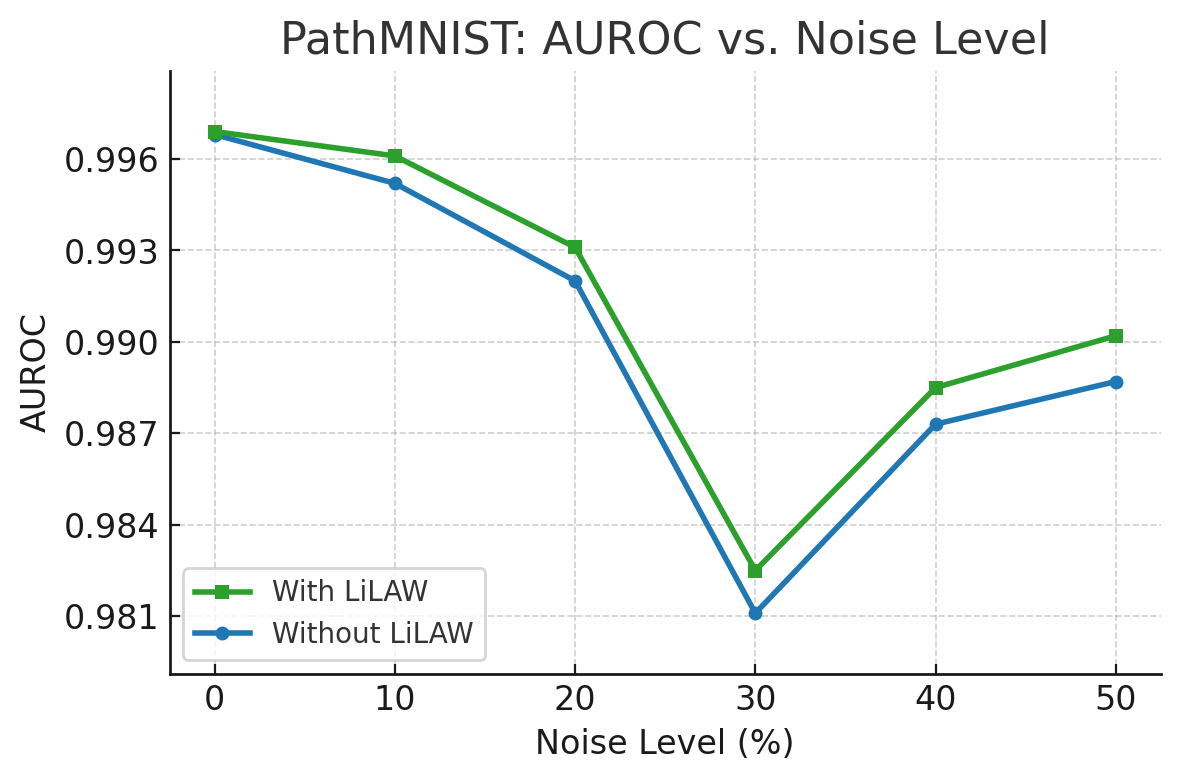
\includegraphics[scale=0.21]{path2.png}
    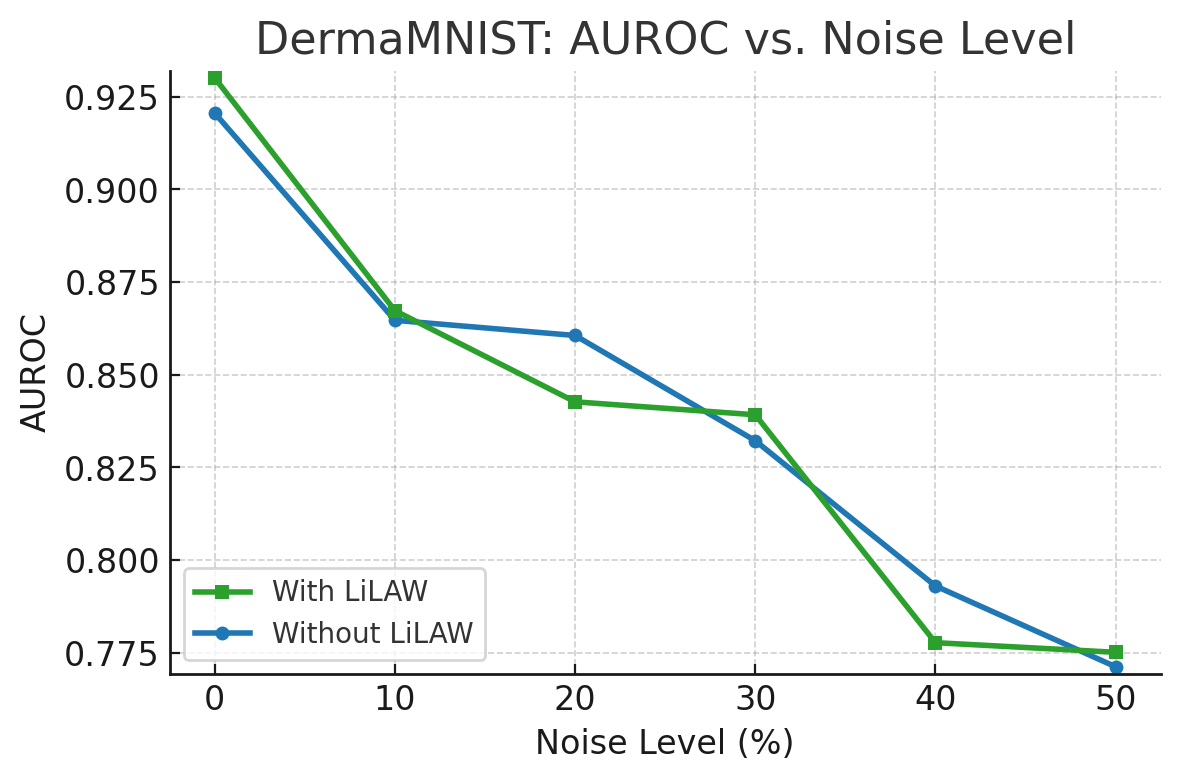
\includegraphics[scale=0.21]{derma2.png}
    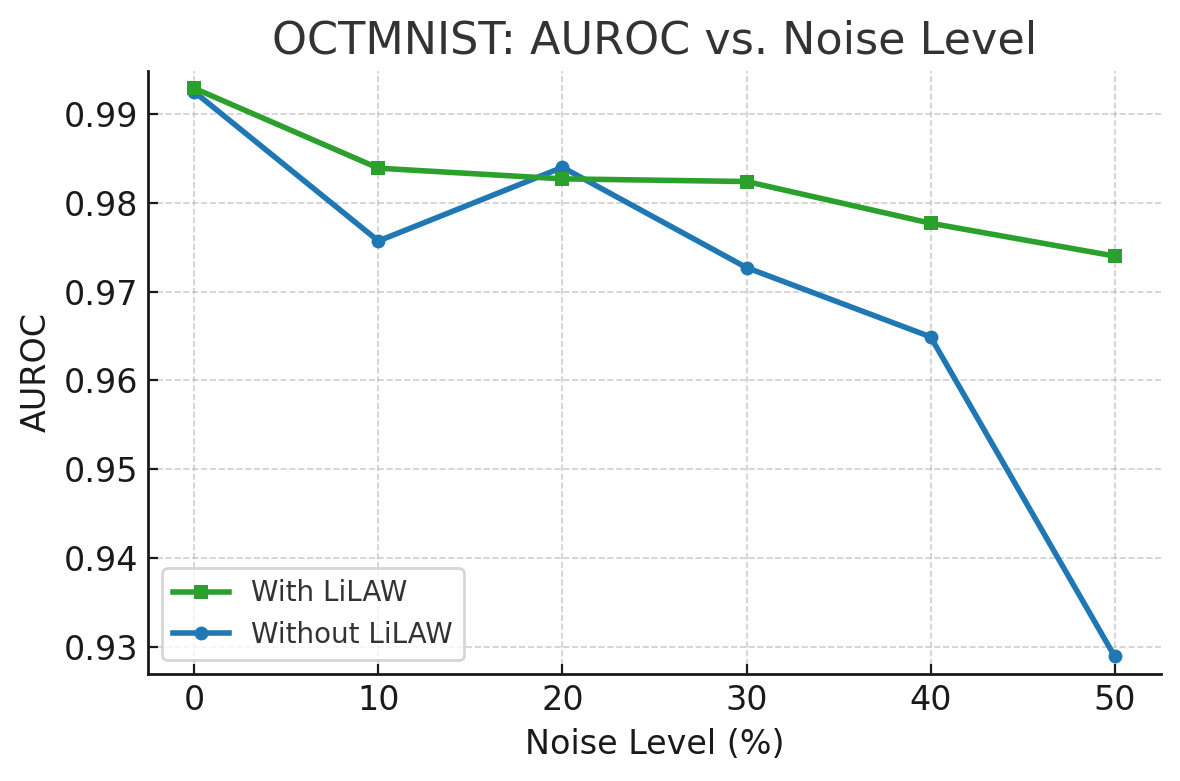
\includegraphics[scale=0.21]{oct2.png}
    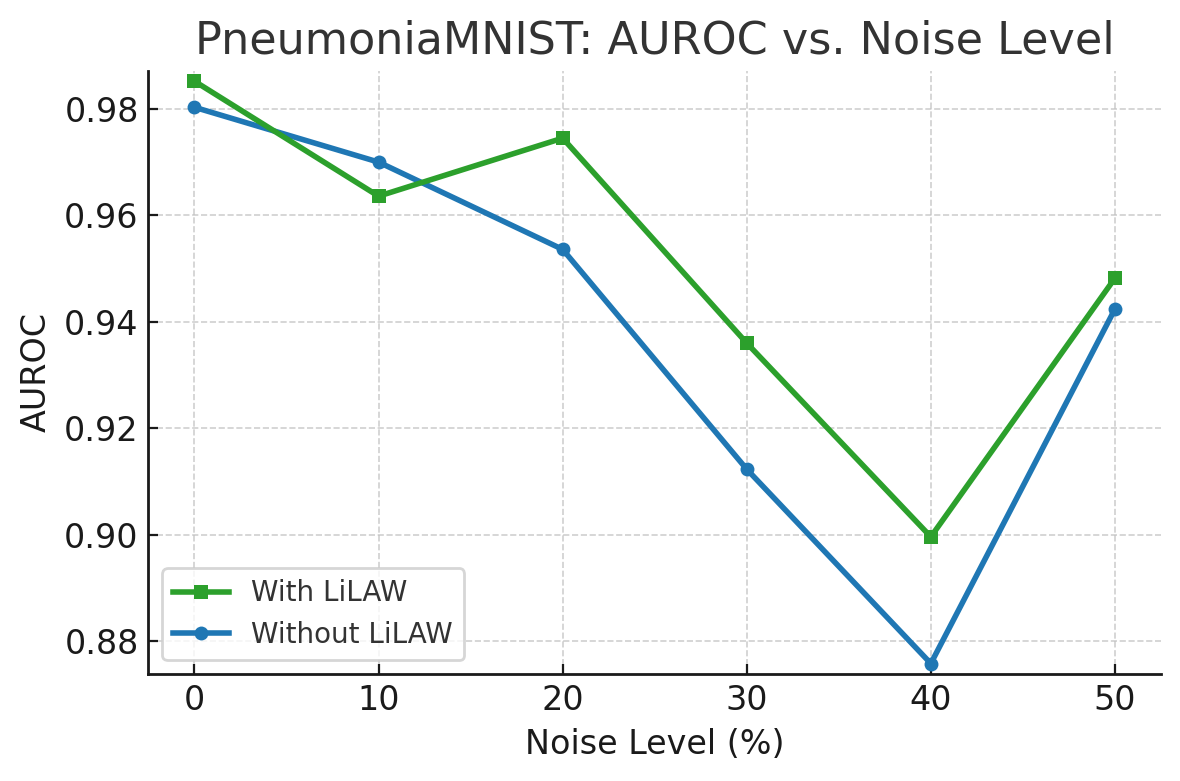
\includegraphics[scale=0.21]{pneumonia2.png}
    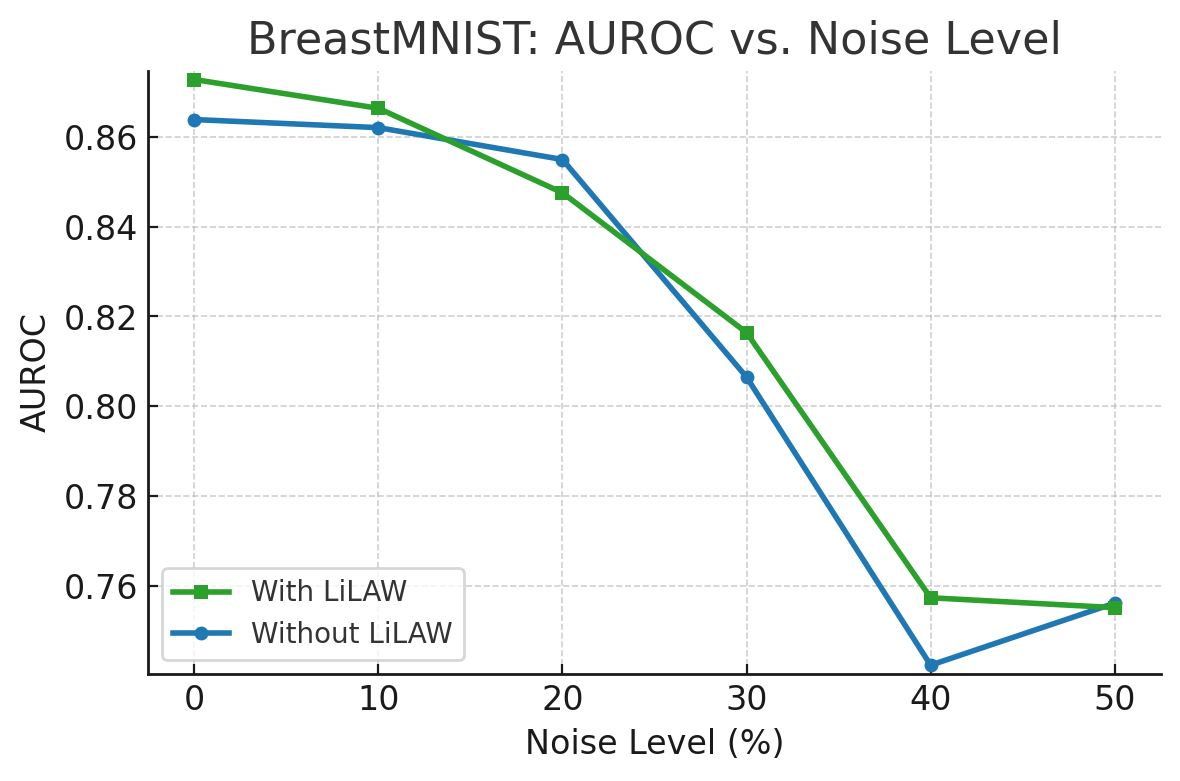
\includegraphics[scale=0.21]{breast2.png}\\
    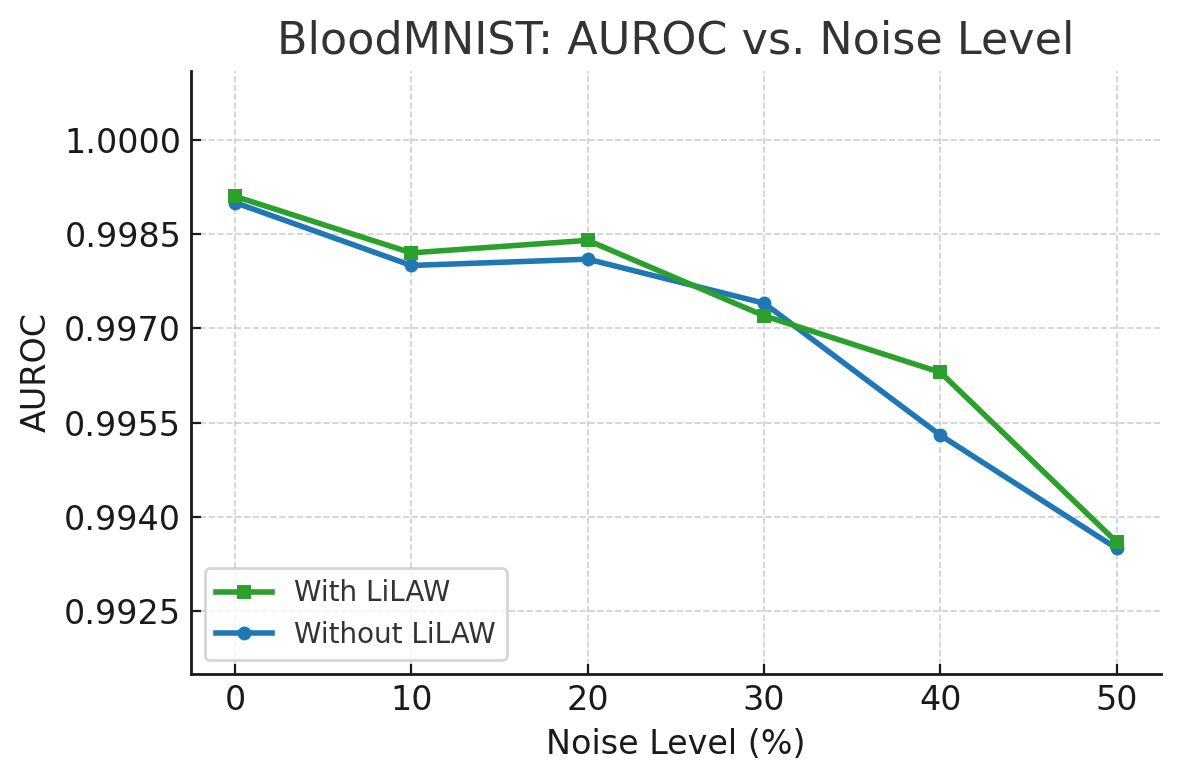
\includegraphics[scale=0.21]{blood2.png}
    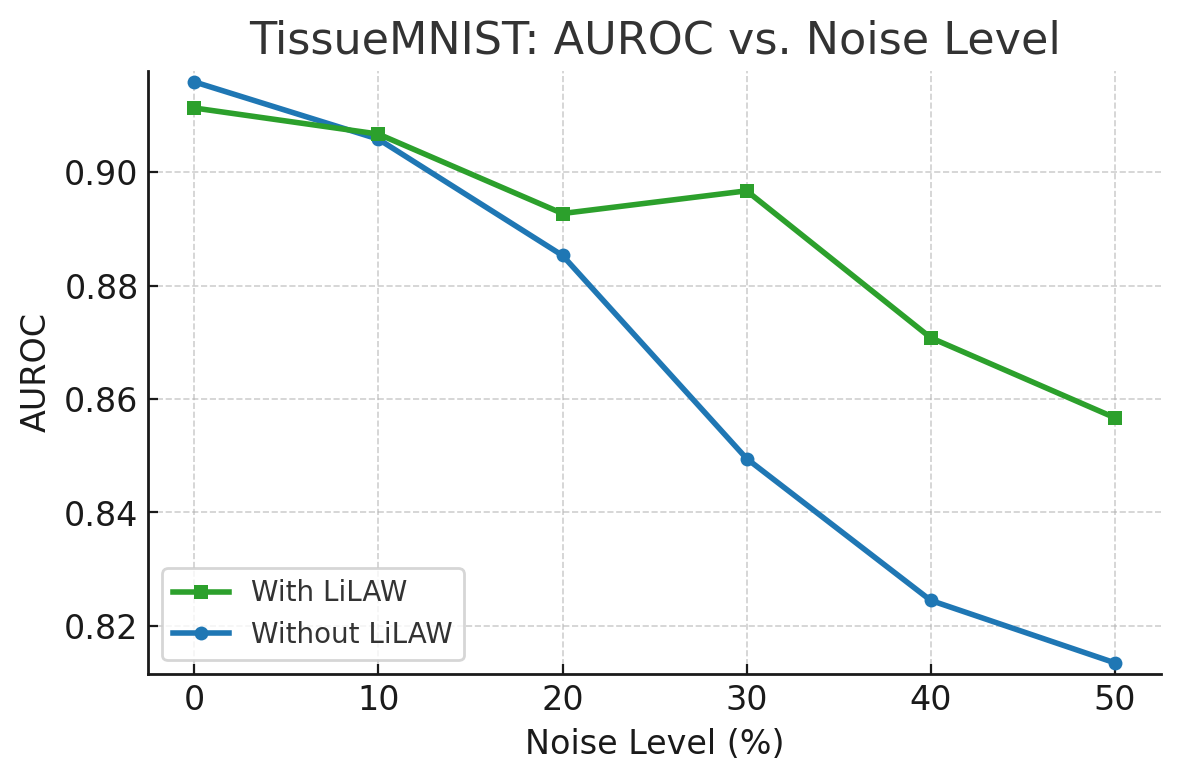
\includegraphics[scale=0.21]{tissue2.png}
    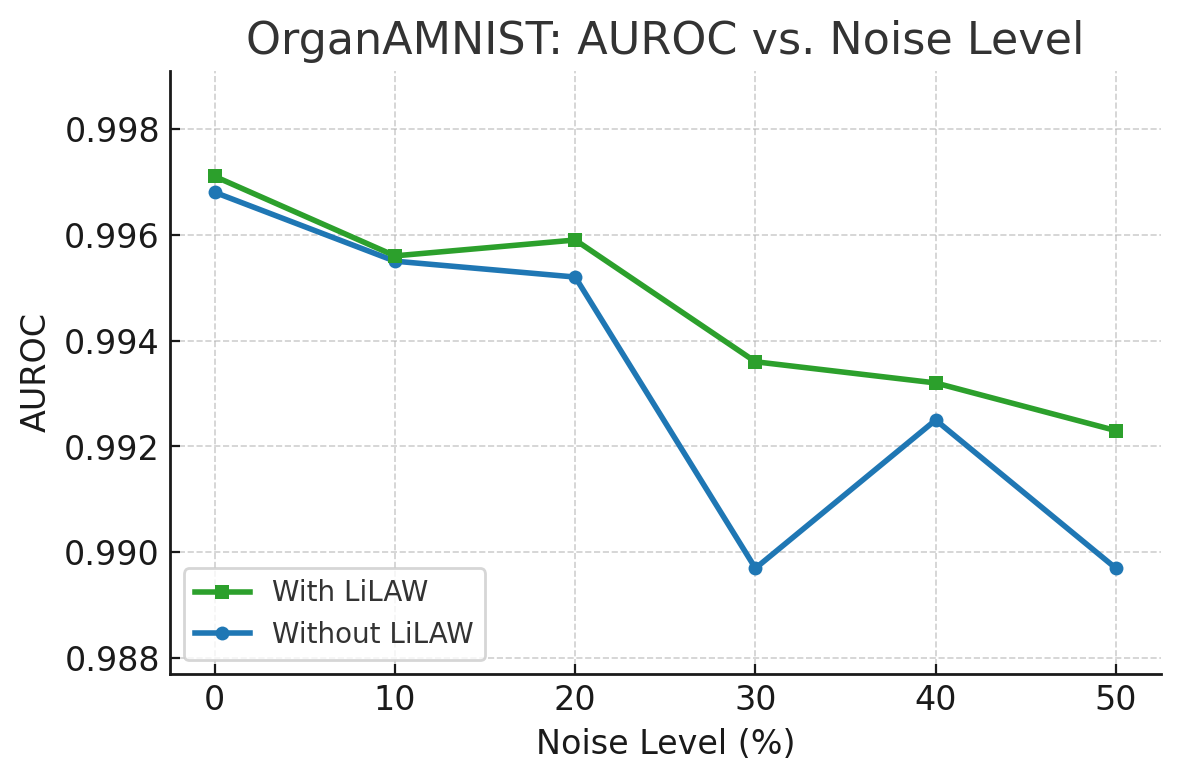
\includegraphics[scale=0.21]{organa2.png}
    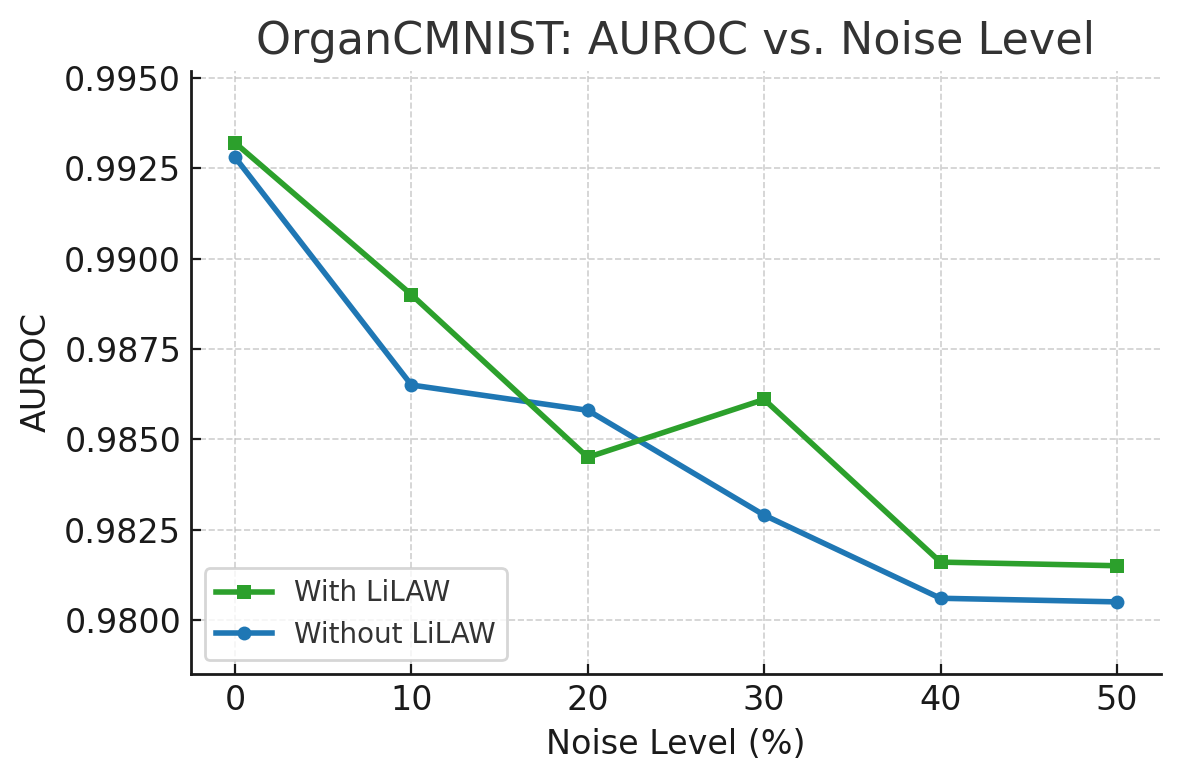
\includegraphics[scale=0.21]{organc2.png}
    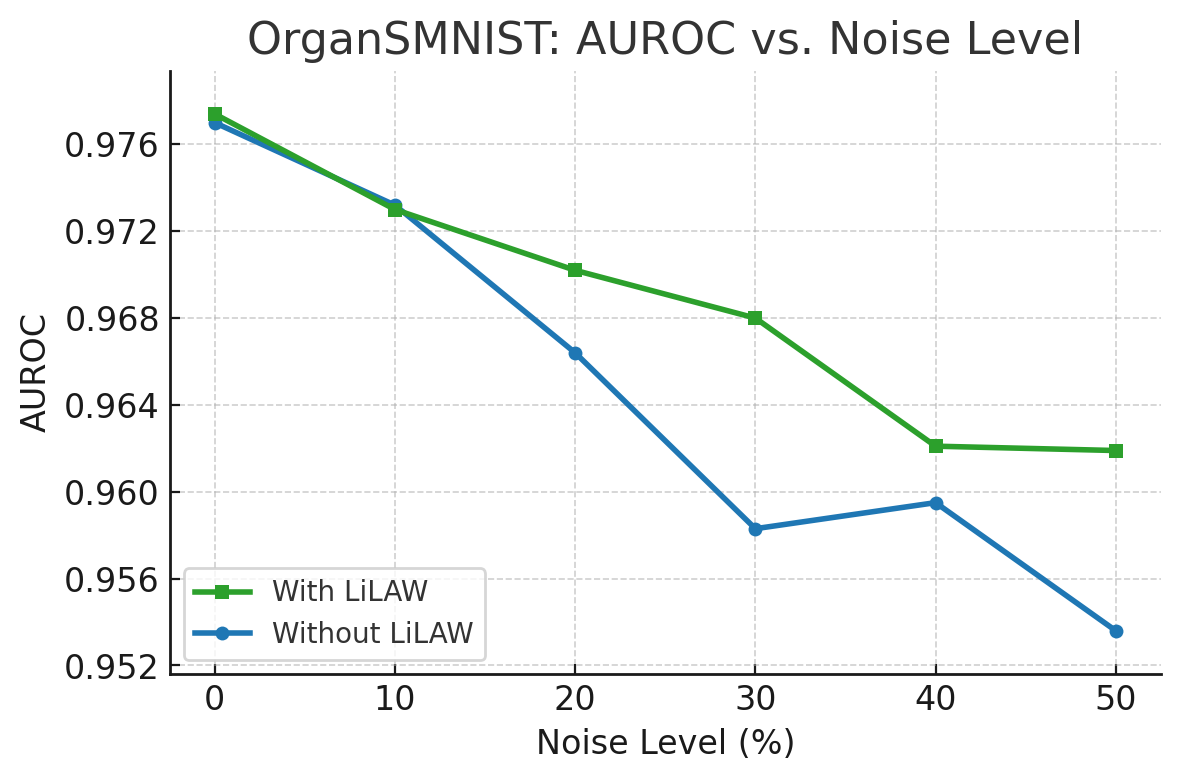
\includegraphics[scale=0.21]{organs2.png}
    \caption{AUROC with and without LiLAW on ten 2D datasets from MedMNISTv2.}
    \label{fig:med2}
\end{figure}
\vspace{-1em}
\subsection{Comparison to baselines for identifying mislabels}
\label{supp:comp}

In Table~\ref{table:comp}, we evaluate mislabel detection on CIFAR-100 with 50\% symmetric noise at an early training stage (epoch~3) and later training stage (epoch~10). Early-stage signals are very informative for LiLAW with $\mathcal{W}_\alpha$ achieving the best AUROC and the best AUPRC at both stages, with minor changes, compared to all 7 other methods. This indicates that, early in training, we can surface mislabeled points and $\mathcal{W}_\alpha$ captures this separation robustly over time. $\mathcal{W}_\beta$ attains high AUROC but low AUPRC, suggesting it ranks many mislabeled items highly but also hard and correct samples highly. $\mathcal{W}_\delta$ improves AUROC with training while maintaining low AUPRC, suggesting that hard samples get easier to identify over time. % but there may be more false positives. %Note that $\mathcal{W}$ takes the sum of $\mathcal{W}_\alpha$, $\mathcal{W}_\beta$, and $\mathcal{W}_\delta$ to aggregate signal from easy, moderate, and hard samples.

\begin{table*}[h!]
\centering
\footnotesize{
\begin{tabular}{l|cc|cc}
\toprule
\multirow{2}{*}{\textbf{Method}} & \multicolumn{2}{c|}{\textbf{AUROC}} & \multicolumn{2}{c}{\textbf{AUPRC}} \\
 & \textbf{Epoch 3} & \textbf{Epoch 10} & \textbf{Epoch 3} & \textbf{Epoch 10} \\
\midrule
Data-IQ \citep{seedat_data-iq_2022}      & 0.9363 & 0.8348 & 0.9290 & 0.9746 \\
DataMaps \citep{swayamdipta_dataset_2020}     & 0.5000 & 0.6989 & 0.5000 & 0.8320 \\
CNLCU-S \citep{xia_sample_2021}        & 0.9438 & 0.9026 & 0.3119 & 0.3181 \\
AUM \citep{pleiss_identifying_2020}        & 0.9680 & 0.9635 & 0.9649 & 0.9610 \\
EL2N \citep{paul_deep_2023}        & 0.9180 & 0.7567 & 0.3161 & 0.3604 \\
GraNd \citep{paul_deep_2023}       & 0.6402 & 0.7034 & 0.4820 & 0.4054 \\
Forgetting \citep{toneva_empirical_2019}  & 0.5000 & 0.5782 & 0.5000 & 0.5740 \\ \midrule
$\mathcal{W}_\alpha$        & \textbf{0.9838} & \textbf{0.9782} & \textbf{0.9810} & \textbf{0.9755} \\
$\mathcal{W}_\beta$         & 0.9719 & 0.9768 & 0.3086 & 0.3085 \\
$\mathcal{W}_\delta$        & 0.8434 & 0.9258 & 0.3454 & 0.3164 \\
$\mathcal{W}$       & 0.7103 & 0.9069 & 0.4985 & 0.3268 \\
\bottomrule
\end{tabular}}
\caption{AUROC and AUPRC comparison of metrics from our method ($\mathcal{W}_\alpha$, $\mathcal{W}_\beta$, $\mathcal{W}_\delta$, $\mathcal{W}$) to identify mislabels (in CIFAR-100 with 50\% symmetric noise) in early-stage (epoch 3) and late-stage (epoch 10) training with 7 other difficulty estimation methods.} % (Note: non-LiLAW metrics were obtained while training without LiLAW).}
\label{table:comp}
\end{table*}

\newpage

\subsection{Pain Detection}
\label{sec:pain}

\textbf{UNBC}-McMaster~\citep{lucey2011painful} (we use UNBC in this paper) contains video data from 25 participants (13 females) with shoulder injuries, recorded during both painful and non-painful movements. The videos were recorded at 30 fps and had a total of 48,391 frames. Each frame is manually annotated with FACS~\citep{ekman1978facial} codes, allowing calculation of the Prkachin and Solomon Pain Intensity (PSPI)~\citep{prkachin2008structure} score. This dataset is publicly available and widely used as a benchmark for pain expression recognition research.

\textbf{UofR}~\citep{rezaei2020unobtrusive} contains video recordings of 102 older adult participants, both with and without dementia. Each session was recorded at 15 fps across two conditions: a baseline lying state and an examination state where a licensed physiotherapist assisted movements to locate painful areas. After removing non-frontal frames, UofR has a total of 162,629 frames. Manual annotations were provided for 95 participants (74 females) using both PSPI and PACSLAC-II pain rating scales, of which 47 cognitively healthy older adults and 48 were residents of long-term care with severe dementia. The test results are reported on the subset of participants with dementia (\textbf{Dementia}) and without dementia (\textbf{Healthy}). Additionally, results on the entire test set are also reported (\textbf{All}). 

\textbf{\synpain}~\citep{taati2025synpain} contains synthetic image pairs consisting of one neutral expression and one expressive image for each identity. Using Ideogram 2.0's commercial API, the authors generated synthetic identities along with their corresponding neutral and expressive image pairs. The dataset encompasses the following demographic and expression categories: age groups include young (20-35) and old (75+); ethnicity/race covers White, Black, South Asian, East Asian, and Middle Eastern; gender represents male and female; expression types span pain (proxy PSPI score of 1) and non-pain (proxy PSPI score of 0). Each synthetic identity comprises two corresponding images (neutral and expressive), with a total of 10,710 images across 5,355 pairs. \textbf{\synpain-Old} refers to the subset of \synpain which only contains images of the old (75+) age group. There are a total of 5,790 images across 2,895 pairs across in \synpain-Old.

\textit{Model.} Pairwise with Contrastive Training (\textbf{PwCT}~\citep{rezaei2020unobtrusive}) is the current state-of-the-art model for detecting painful expressions in older adults. It is trained on UNBC and UofR datasets for regression (so we use R=16 since PSPI $\in [0,16]$, as mentioned in \ref{sec:regression}), but we threshold the results to obtain binary pain classification. The two key ideas of PwCT are personalized neutral baselines comparing each test expression to that person's own neutral face to reduce age-related idiosyncrasies and contrastive representation learning to improve cross-dataset generalization. The model has been externally validated in vivo and is currently being evaluated in situ. We use the pre-trained PwCT model and fine-tune it with \synpain in this paper using the setup described in~\citet{rezaei2020unobtrusive}.

\begin{table*}[h!]
\centering
\begin{footnotesize}{
\begin{tabular}{cc|ccc}
\toprule
 \multicolumn{2}{c}{\textbf{Dataset configurations}} & \multicolumn{3}{c}{\textbf{AUROC}} \\ \midrule
\textbf{Training} & \textbf{Meta-validation (LiLAW)} & \textbf{Dementia} & \textbf{Healthy} & \textbf{All} \\ \midrule
UofR, UNBC & - & \textbf{0.787} & 0.763 & 0.775 \\ \midrule
& - & 0.761 & 0.774 & 0.767 \\
UofR, UNBC, \synpain & UofR & 0.767 & 0.801 & 0.784 \\
& UofR, \synpain & 0.778 & 0.794 & 0.786 \\ \midrule
& - & 0.778 & 0.779 & 0.778 \\
& UofR, \synpain-Old & 0.782 & 0.796 & \textbf{0.789} \\
UofR, UNBC, \synpain-Old  & UofR, UNBC, \synpain-Old & 0.763 & 0.796 & 0.780 \\
 & \synpain-Old & 0.754 & \textbf{0.803} & 0.779 \\
 & UofR & \textbf{0.784} & \textbf{0.803} & \textbf{0.793} \\
\bottomrule
\end{tabular}}
\caption{Results of fine-tuning the PwCT model with and without LiLAW under different dataset configurations (UofR, UNBC, \synpain, and \synpain-Old). The top 2 results from each column of the UofR test set (Dementia, Healthy, and All) are in \textbf{bold}.}
\label{x}
\end{footnotesize}
\end{table*}
\vspace{-2em}
The results on pain classification in Table~\ref{x} demonstrate the interaction between heterogeneous real datasets, synthetic data augmentations, and LiLAW within the PwCT framework. When trained only on UofR and UNBC, PwCT achieves strong baseline AUROC on the Dementia subgroup (0.787), but relatively weaker performance on Healthy participants (0.763). Incorporating synthetic data from \synpain or \synpain-Old without LiLAW gives inconsistent results: while Healthy AUROC occasionally improves, Dementia AUROC and All AUROC often stagnate or decline, suggesting that naively combining real and synthetic samples risks degradation. With LiLAW, however, meta-validation effectively reweighs real and synthetic examples. The best outcome is observed when training on UofR, UNBC, and \synpain-Old while meta-validating on UofR, resulting in AUROCs of 0.784 (Dementia), 0.803 (Healthy), and 0.793 (All). These results highlight that LiLAW selectively downweighs misleading or difficult synthetic samples. We also achieve state-of-the-art results on the UofR test set. LiLAW enables PwCT to integrate synthetic data in a controlled and clinically meaningful way.

\subsection{Gait classification}
\label{sec:gait}
\textbf{PD-GaM}~\citep{adeli2025gaitgen} is a fully anonymized, publicly available 3D mesh dataset of parkinsonian gait derived from PD4T~\citep{dadashzadeh2023pecopparameterefficientcontinual}. It contains 1,701 segmented walking sequences from 30 individuals with Parkinson's disease, each labeled by an expert with UPDRS-gait scores from 0 to 3 (score 4 is typically non-ambulatory). Sequences are extracted from video at 25 fps, with post-processing to correct global trajectory artifacts. PD-GaM is the largest public UPDRS-gait-annotated mesh dataset, designed to mitigate data scarcity (especially at higher severities) and to support clinically relevant evaluation metrics. We use the validation set for LiLAW's meta-validation.

\textbf{\gaitgen}~\citep{adeli2025gaitgen} is a generative framework that synthesizes realistic gait sequences conditioned on Parkinson's severity (UPDRS-gait scores from 0 to 3). It disentangles motion dynamics from pathology using a Conditional Residual VQ-VAE, then generates base sequences with a Mask Transformer and refines details via a Residual Transformer, enabling precise control over impairment level. Clinician studies report near-chance discrimination between real and synthetic clips.

\textit{Model.} We use the \textbf{MotionClassifier}~\citep{adeli2025gaitgen} model to train a lightweight supervised head on a fixed 512-D motion embeddings extracted from each gait sequence by the evaluation backbone. The classifier is a 3-layer MLP that produces class logits optimized using Adam for 7000 epochs with batch size 256 and learning rate 0.00001 when synthetic data is used and 0.0001 when synthetic data is not used. We train the MLP from scratch using the same setup as before.

\begin{table*}[h!] \centering
\begin{tabular}{c|ccc}
\hline
\textbf{Dataset} & \textbf{Recall} & \textbf{Precision} & \textbf{Macro-F1} \\
\hline
PD-GaM & 70.09 \textcolor{Green}{$\uparrow$} 0.03\hspace{0.5em} & 75.32 \textcolor{Green}{$\uparrow$} 1.15\hspace{0.5em} & 70.29 \textcolor{Green}{$\uparrow$} 0.98\hspace{0.5em} \\
PD-GaM + \gaitgen & 73.94 \textcolor{Green}{$\uparrow$} 3.51\hspace{0.5em} & 80.20 \textcolor{Green}{$\uparrow$} 1.17\hspace{0.5em} & 75.95 \textcolor{Green}{$\uparrow$} 2.60\hspace{0.5em} \\
\hline
\end{tabular}
\caption{Results of the MotionClassifier model with PD-GaM and with both PD-GaM + \gaitgen without LiLAW along with the increase (signified by \textcolor{Green}{$\uparrow$}) in performance with LiLAW.}
\label{tab:gait}
\end{table*}

\iffalse
\begin{figure}
    \centering
    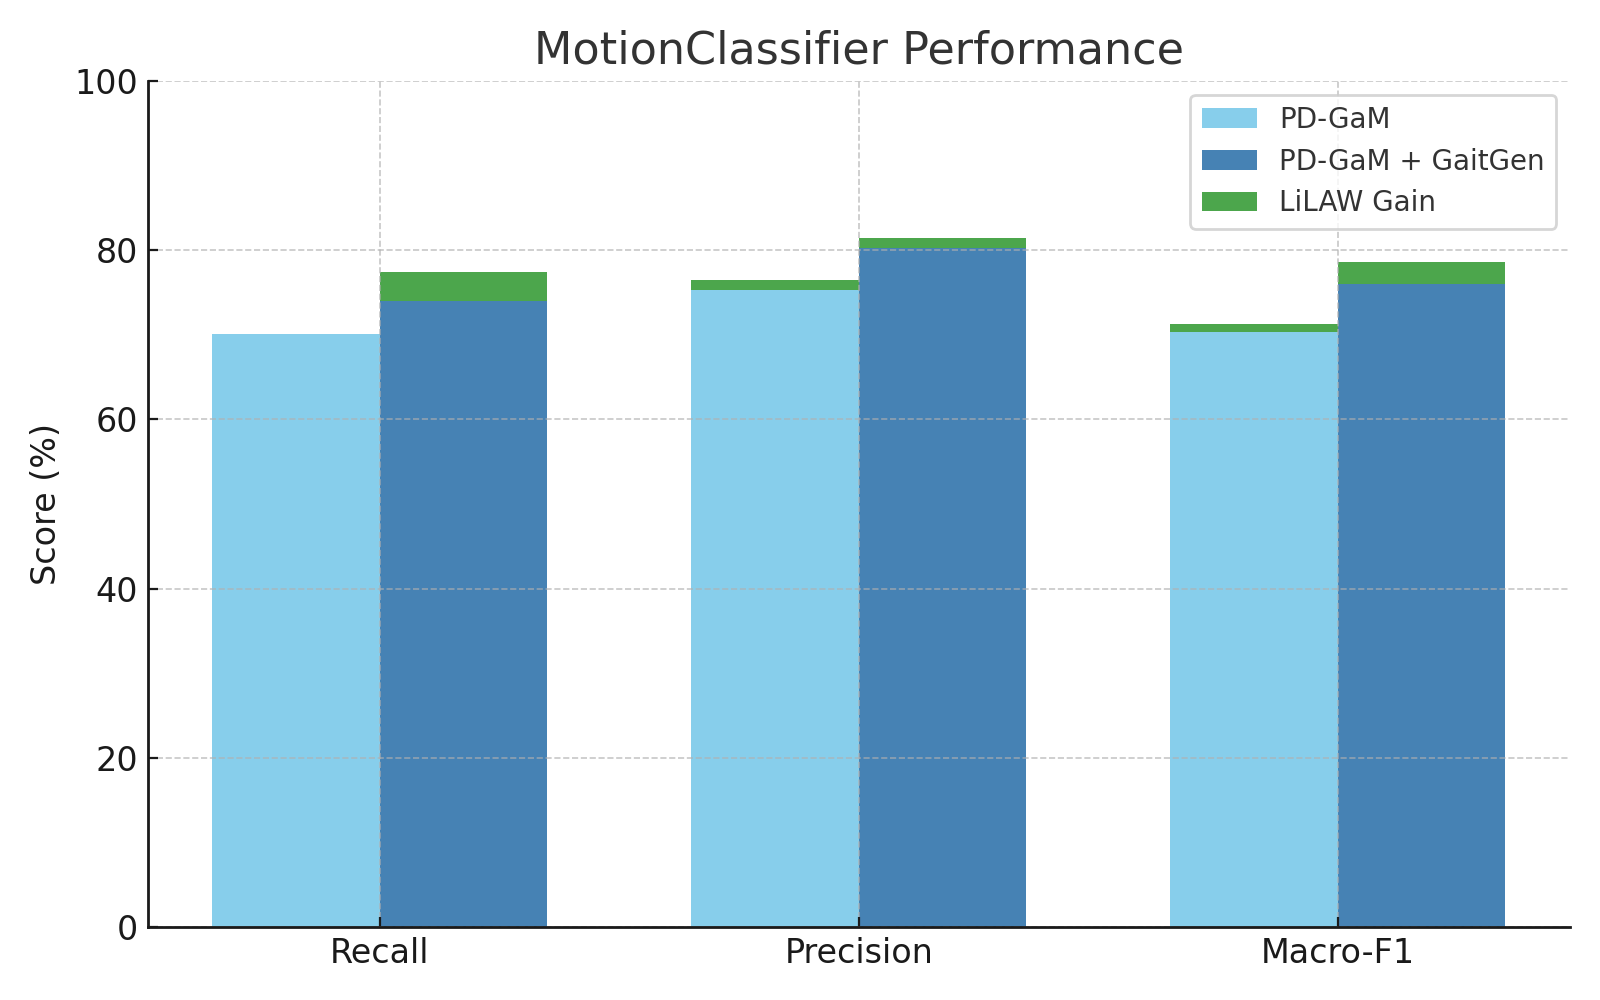
\includegraphics[scale=0.4]{motionclassifier.png}
    \caption{Recall, precision, and macro-F1 scores of the MotionClassifer with and without synthetic data and with and without LiLAW.}
    \label{fig:motionclassifier}
\end{figure}
\fi 
\vspace{-1.5em}
In the gait classification task, Table~\ref{tab:gait} shows how LiLAW enhances the MotionClassifier trained on PD-GaM and synthetic gait sequences generated by \gaitgen. On PD-GaM alone, the MotionClassifier achieves recall of 70.09, precision of 75.32, and macro-F1 of 70.29. With LiLAW, each metric improves modestly, stabilizing training even without synthetic data. However, when synthetic \gaitgen samples are introduced, baseline performance rises substantially to a recall of 73.94, precision of 80.20, macro-F1 of 75.95, but LiLAW amplifies these gains even further, with recall increasing by 3.51, precision by 1.17, and macro-F1 by 2.60. These results achieve state-of-the-art for the PD-GaM test dataset. These gains are especially important clinically, as recall corresponds to sensitivity in detecting higher-severity Parkinsonian gait impairments. Rather than overfitting to synthetic distributions, LiLAW leverages them and demonstrates that synthetic augmentation paired with LiLAW can help improve subgroup generalization.
\vspace{-0.5em}
\subsection{Heartbeat classification}
\label{sec:heart}
\textbf{ECG5000}~\citep{goldberger2000physiobank} is a five-class heartbeat dataset derived from a single 20-hour ECG tracing in the BIDMC Congestive Heart Failure Database (in PhysioNet). The preprocessing isolates individual heartbeats and interpolates each to a fixed length. 5,000 heartbeats are then randomly selected. Labels are obtained via automated annotation. We reserve 5\% of the training set for LiLAW's meta-validation.

To introduce variability and simulate sensor and physiological noise, we augment 50\% of the training heartbeats with additive Gaussian perturbations that combine a random offset and stochastic variance. We call this augmented dataset \textbf{ECG5000-A}. For a heartbeat sequence $x$, the augmented sample is:
\[
\tilde{x} \;=\; x \;+\; b \;+\; \sigma \varepsilon,\quad
b \sim \mathcal{U}[-0.2,\,0.2],\ \ \sigma=\sqrt{u},\ u \sim \mathcal{U}[0.05,\,0.1],\ \ \varepsilon \sim \mathcal{N}(0,I).
\]
Class labels are retained for augmented samples.

\textit{Model.} We train on ECG5000 using a simple \textbf{Stacked LSTM} model (containing 2 LSTM layers) from scratch. We use the Adam optimizer for 500 epochs with batch size 512 and learning rate 0.001. %We train the model using the same setup as before.

\begin{table}[ht]
\begin{footnotesize}
\centering
\begin{tabular}{c|cc}
\hline
\textbf{Dataset} & \textbf{Acc. (\%)} & \textbf{AUROC} \\
\hline
ECG5000 & 93.60 \textcolor{Green}{$\uparrow$} 3.20 & 0.9982 \textcolor{Green}{$\uparrow$} 0.0005 \\
ECG5000-A & 96.80 \textcolor{Green}{$\uparrow$} 3.20 & 0.9907 \textcolor{Green}{$\uparrow$} 0.0093 \\
\hline
\end{tabular}
\caption{Results of the Stacked LSTM model with ECG5000 and with ECG5000-A without LiLAW along with the increase (signified by \textcolor{Green}{$\uparrow$}) in performance with LiLAW.}
\label{tab:ecg}
\end{footnotesize}
\end{table}

\iffalse
\begin{figure}
    \centering
    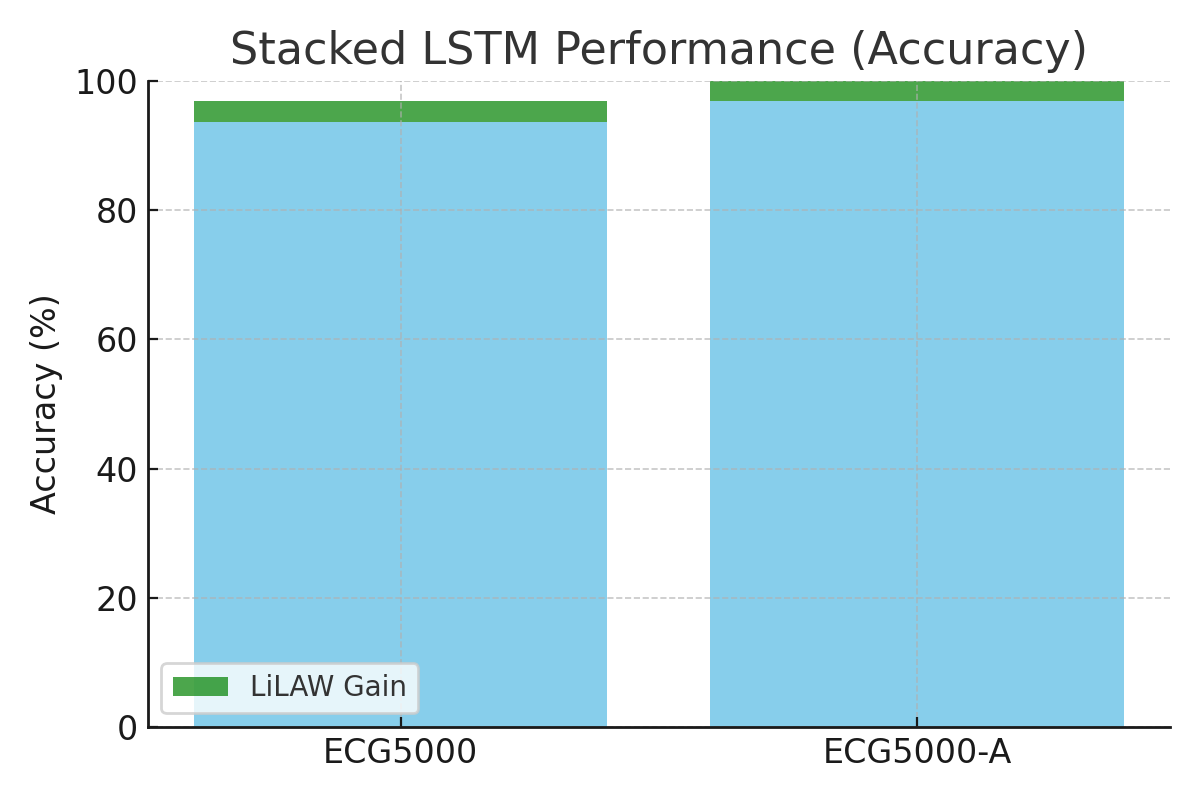
\includegraphics[scale=0.4]{ecg5000_accuracy.png}
    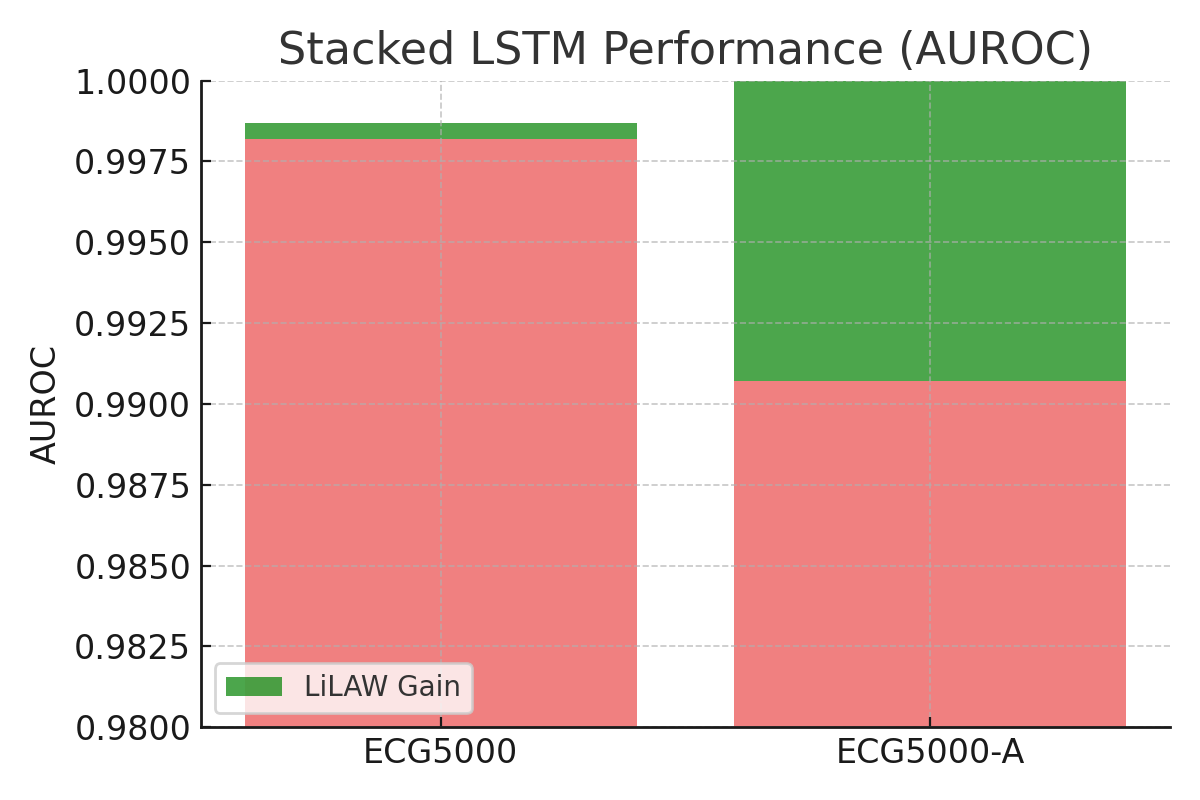
\includegraphics[scale=0.4]{ecg5000_auroc.png}
    \caption{Accuracy and AUROC of Stacked LSTM model with and without augmented data and with and without LiLAW.}
    \label{fig:ecg5000}
\end{figure}
\fi

The ECG heartbeat classification results in Table~\ref{tab:ecg} highlight LiLAW's utility in time-series domains where baseline performance is already saturated. Using a Stacked LSTM trained from scratch, ECG5000 alone achieves 93.60\% accuracy and an AUROC of 0.9982. Even in this high-performing setting, LiLAW yields improvements (accuracy up by 3.20\%, AUROC  up by 0.0005). When training on ECG5000-A, which contains classical data augmentations, accuracy increases to 96.80\%, but AUROC drops to 0.9907, suggesting that the augmentation increases accuracy but decreases confidence. LiLAW mitigates this imbalance by improving the AUROC by 0.0093 while preserving accuracy gains. These results achieve state-of-the-art for the ECG5000 test dataset.

Compared to standard training, LiLAW yields a substantial improvement in accuracy and AUROC, demonstrating its ability to enhance predictive performance and discrimination in inherently noisy domains. Namely, LiLAW can dynamically reweight samples based on difficulty to effectively mitigate the impact of inherent noise in physiological signals. This suggests that LiLAW provides a generalizable framework to improve robustness across modalities where label quality and data heterogeneity are common challenges.

\vspace{-0.5em}
\subsection{Improving Fairness}
\label{fairness}

Using the Adult dataset for income prediction with a 70-30 train-test split (with 10\% of the training set used for validation), we study how using LiLAW on a 3-layer MLP generally improves performance and fairness across five different common fairness metrics~\cite{garg2020fairness}. We first report the performance boost when we use LiLAW in Table~\ref{tab:adult}.

\newcommand{\Up}{\textcolor{Green}{\ensuremath{\uparrow}}}
\newcommand{\Upr}{\textcolor{BrickRed}{\ensuremath{\uparrow}}}
\newcommand{\Downg}{\textcolor{Green}{\ensuremath{\downarrow}}}
\newcommand{\Down}{\textcolor{BrickRed}{\ensuremath{\downarrow}}}
\newcommand{\Eq}{\textcolor{gray}{\ensuremath{\leftrightarrow}}}

\begin{table}[ht]
\centering
\small
\begin{subtable}{}
\centering
\begin{tabular}{cc}
\toprule
Accuracy & Support \\
\midrule
0.8541 \textcolor{Green}{\ensuremath{\uparrow}} 0.0026 & 9769 \\
\bottomrule
\end{tabular}
%\caption{Overall accuracy}
\end{subtable}

\vspace{0.1em}

\begin{subtable}{}
\centering
\begin{tabular}{lcccr}
\toprule
Class & Precision & Recall & F1-score & Support \\
\midrule
$\leq$50K
& 0.8827 \textcolor{Green}{\ensuremath{\uparrow}} 0.0002
& 0.9316 \textcolor{Green}{\ensuremath{\uparrow}} 0.0037
& 0.9065 \textcolor{Green}{\ensuremath{\uparrow}} 0.0018
& 7417 \\

$>$50K
& 0.7388 \textcolor{Green}{\ensuremath{\uparrow}} 0.0102
& 0.6097 \textcolor{BrickRed}{\ensuremath{\downarrow}} 0.0009
& 0.6681 \textcolor{Green}{\ensuremath{\uparrow}} 0.0036
& 2352 \\

\midrule
Average &  &  &  &  \\
\midrule
Macro average
& 0.8108 \textcolor{Green}{\ensuremath{\uparrow}} 0.0051
& 0.7707 \textcolor{Green}{\ensuremath{\uparrow}} 0.0014
& 0.7873 \textcolor{Green}{\ensuremath{\uparrow}} 0.0027
& 9769 \\

Weighted average
& 0.8481 \textcolor{Green}{\ensuremath{\uparrow}} 0.0026
& 0.8541 \textcolor{Green}{\ensuremath{\uparrow}} 0.0026
& 0.8491 \textcolor{Green}{\ensuremath{\uparrow}} 0.0023
& 9769 \\
\bottomrule
\end{tabular}
\end{subtable}

\caption{Performance metrics for the Adult dataset trained with a 3-layer MLP. For each metric, the left value shows the metric without LiLAW, and the right value shows the change with LiLAW. Upward arrows indicate increases, while downward arrows indicate decreases.}
\label{tab:adult}
\end{table}
\vspace{-1.5em}
We see a consistent improvement in performance, with an increase in the accuracy and the macro and weighted averages of precision, recall, and F1-score. While the $\leq$50K class sees consistent improvements since it is the majority label, the $>$50K class exhibits higher precision and F1-score at the cost of a small decrease in recall.

Now, let $A$ be a sensitive attribute, $Y\in\{0,1\}$ be the true label, and $\hat{Y}$ be the prediction. The disparity in the metrics relative to a reference group $r$ for each group $g \neq r$ is: $\Delta m_g = m_g - m_r$. Predictions are fairer when $\Delta m_g$ is near 0. Note: For sex, $r =$ Male. For race, $r =$ White. For age, $r =$ 45--54. These categories have the highest income in the Adult dataset.

We report the disparities in disadvantaged groups (based on sensitive attribute) relative to the reference group or privileged group with and without LiLAW for sex, race, and age in Tables~\ref{tab:sex},~\ref{tab:race}, and~\ref{tab:age}, respectively. We consider five fairess metrics:
\begin{enumerate}
\vspace{-0.3em}
    \item $\Delta DP_g = DP_g - DP_r$, where $DP_a = \Pr(\hat{Y}=1|A=a)$\newline
    This measures the change in \textit{demographic parity}, i.e. positive prediction rates are similar across two groups.
\vspace{-0.3em}
    \item $\Delta TPR_g = TPR_g - TPR_r$, where $TPR_a = \Pr(\hat{Y}=1|Y=1,A=a)$\newline
    This measures the change in the true positive rate and is referred to as \textit{equal opportunity} when it is equal across groups, i.e. true positives are identified at similar rates across two groups.
\vspace{-0.3em}
    \item $\Delta FPR_g = FPR_g - FPR_r$, where $FPR_a = \Pr(\hat{Y}=1|Y=0,A=a)$\newline
    This measures the change in the false positive rate, i.e. false positives are mistakenly identified at similar rates across two groups. Note that combining 2 and 3 gives us \textit{equalized odds}.
\vspace{-0.3em}
    \item $\Delta PPV_g = PPV_g - PPV_r$, where $PPV_a = \Pr(Y=1|\hat{Y}=1,A=a)$\newline
    This measures the change in the positive prediction value and is referred to as \textit{predictive parity}, i.e. probability of a positive outcome given a positive prediction is similar across two groups.
\vspace{-0.3em}
    \item $\Delta ACC_g = ACC_g - ACC_r$, where $ACC_a = \Pr(Y=\hat{Y}|A=a)$\newline
    This measures the change in accuracy and is referred to as \textit{accuracy parity}, i.e. accuracy is similar across two groups.
\end{enumerate}

\begin{table}[h!]
\centering
\scriptsize
\setlength{\tabcolsep}{3pt}
\renewcommand{\arraystretch}{1.15}
{%
\begin{tabular}{lrccccc}
\toprule
sex & n & $\Delta\,DP$ & $\Delta\,TPR$ & $\Delta\,FPR$ & $\Delta\,PPV$ & $\Delta\,ACC$ \\
\midrule
Male   & 6537 & $-$ & $-$ & $-$ & $-$ & $-$ \\
Female & 3232 & $\,-0.1712\,\Up\,0.0086\,$ & $\,-0.0522\,\Up\,0.0277\,$ & $\,-0.0703\,\Up\,0.0065\,$ & $\,-0.0083\,\Down\,0.0061\,$ & $\,0.1135\,\Downg\,0.0006\,$ \\
\bottomrule
\end{tabular}%
}
\caption{Fairness disparities by sex relative to the reference group (Male) in the Adult Dataset trained with a 3-layer MLP. For each metric, the left value shows the disparity without LiLAW, and the right value shows the magnitude of the change with LiLAW. Upward arrows indicate that the metric increased with LiLAW, while downward arrows indicate a decrease. Green arrows indicate decreased disparity and red arrows indicate increased disparity.}
\label{tab:sex}
\end{table}

\begin{table}[h!]
\centering
\scriptsize
\setlength{\tabcolsep}{3pt}
\renewcommand{\arraystretch}{1.15}
{%
\begin{tabular}{lrccccc}
\toprule
race & n & $\Delta\,DP$ & $\Delta\,TPR$ & $\Delta\,FPR$ & $\Delta\,PPV$ & $\Delta\,ACC$\\
\midrule
White              & 8304 & $-$ & $-$ & $-$ & $-$ & $-$ \\
Black              & 968  & $\,-0.1211\,\Up\,0.0062\,$ & $\,-0.0742\,\Up\,0.0005\,$ & $\,-0.0411\,\Up\,0.0076\,$ & $\,-0.0471\,\Down\,0.0341\,$ & $\,0.0718\,\Downg\,0.0060\,$\\
Asian-Pac-Islander & 331  & \hspace{1em}$\,0.0398\,\Downg\,0.0059\,$ & $\,-0.0307\,\Up\,0.0124\,$ & \hspace{1em}$\,0.0662\,\Downg\,0.0121\,$ & $\,-0.1579\,\Up\,0.0239\,$ & \hspace{-1em}$\,-0.0561\,\Up\,0.0122\,$\\
Amer-Indian%-Eskimo
& 94   & $\,-0.0727\,\Down\,0.0289\,$ & \hspace{1em}$\,0.0288\,\Down\,0.1424\,$ & $\,-0.0215\,\Down\,0.0084\,$ & $\,-0.0560\,\Down\,0.0030\,$ & $\,0.0566\,\Downg\,0.0135\,$\\
Other              & 72   & $\,-0.1276\,\Up\,0.0031\,$ & \hspace{1em}$\,0.0526\,\Up\,0.0005\,$ & $\,-0.0412\,\Up\,0.0041\,$ & $\,-0.0816\,\Down\,0.0107\,$ & $\,0.0968\,\Downg\,0.0029\,$\\
\bottomrule
\end{tabular}%
}
\caption{Fairness disparities by race relative to the reference group (White) in the Adult Dataset trained with a 3-layer MLP. For each metric, the left value shows the disparity without LiLAW, and the right value shows the magnitude of the change with LiLAW. Upward arrows indicate that the metric increased with LiLAW, while downward arrows indicate a decrease. Green arrows indicate decreased disparity and red arrows indicate increased disparity.}
\label{tab:race}
\end{table}

\begin{table}[h!]
\centering
\scriptsize
\setlength{\tabcolsep}{3pt}
\renewcommand{\arraystretch}{1.15}
{%
\begin{tabular}{lrccccc}
\toprule
age & n & $\Delta\,DP$ & $\Delta\,TPR$ & $\Delta\,FPR$ & $\Delta\,PPV$ & $\Delta\,ACC$\\
\midrule
$\leq 24$     & 1658 & $\,-0.3456\,\Up\,0.0110\,$ & $\,-0.3295\,\Up\,0.0100\,$ & $\,-0.1391\,\Up\,0.0116\,$ & \hspace{1em}$\,0.0960\,\Downg\,0.0127\,$ & $\,0.2112\,\Downg\,0.0029\,$\\
25--34        & 2621 & $\,-0.2411\,\Up\,0.0102\,$ & $\,-0.2065\,\Up\,0.0123\,$ & $\,-0.1024\,\Up\,0.0102\,$ & $\,-0.0453\,\Down\,0.0041\,$ & $\,0.0954\,\Downg\,0.0014\,$ \\
35--44        & 2401 & $\,-0.0450\,\Up\,0.0076\,$ & \hspace{1em}$\,0.0185\,\Upr\,0.0126\,$ & $\,-0.0208\,\Up\,0.0053\,$ & $\,-0.0220\,\Down\,0.0018\,$ & $\,0.0341\,\Upr\,0.0021\,$  \\
45--54        & 1735 & $-$ & $-$ & $-$ & $-$ & $-$ \\
55--64        & 947  & $\,-0.0859\,\Up\,0.0078\,$ & $\,-0.0951\,\Up\,0.0100\,$ & $\,-0.0235\,\Up\,0.0069\,$ & $\,-0.0571\,\Down\,0.0041\,$ & \hspace{-1em}$\,-0.0006\,\Up\,0.0003\,$  \\
$65+$         & 407  & $\,-0.2024\,\Up\,0.0183\,$ & $\,-0.1396\,\Up\,0.0333\,$ & $\,-0.0930\,\Up\,0.0147\,$ & $\,-0.0111\,\Down\,0.0167\,$ & $\,0.0814\,\Downg\,0.0004\,$  \\
\bottomrule
\end{tabular}%
}
\caption{Fairness disparities by age relative to the reference group (45--54) in the Adult Dataset trained with a 3-layer MLP. For each metric, the left value shows the disparity without LiLAW, and the right value shows the magnitude of the change with LiLAW. Upward arrows indicate that the metric increased with LiLAW, while downward arrows indicate a decrease. Green arrows indicate decreased disparity and red arrows indicate increased disparity.}
\label{tab:age}
\end{table}

We see in Tables~\ref{tab:sex},~\ref{tab:race}, and~\ref{tab:age} that we compare each group in each table to a privileged reference group, where values closer to 0 imply smaller disparities. In general, adding LiLAW tends to move nearly all non-reference group disparities closer to 0 for improve demographic parity, equalized odds (inc. equal opportunity), and accuracy parity. However, some groups have an increase in predictive parity with LiLAW, since it is generally impossible to simultaneously achieve demographic parity, equalized odds, and predictive parity due to the impossibility theorem~\citep{imposs}. Also, results from very small groups should be treated cautiously since they can fluctuate more, although in our case, we still see some improvements.

\subsubsection{Proof that LiLAW helps improve performance and fairness}

Intuitively, each sample loss is multiplied by a differentiable weight
$\mathcal{W}(s_i,\tilde y_i)$ that depends on $s_i[\tilde y_i]$ and $\max(s_i)$ as mentioned in Sec.~\ref{sec:method}. Since $\mathcal{W}(s_i,\tilde y_i)$ is designed and updated to emphasize unconfidence and/or disagreement with the observed label, optimization focuses more on informative hard and moderate examples while reducing the influence of very easy points, which typically improves generalization. On the other hand, since underrepresented groups contain a higher fraction of these harder cases (due to imbalance, label noise, or distribution shift), LiLAW implicitly increases their training signal. As a result, we reduce disparities in fairness metrics while often improving overall performance.

\begin{proposition}
Assume that LiLAW assigns larger weights to samples that are hard and moderate (low $s_i[\tilde y_i]$ and/or disagreement with $\max(s_i)$) and that such examples occur more frequently in disadvantaged groups, as shown empirically in Tables~\ref{tab:sex},~\ref{tab:race},~\ref{tab:age}. Then, minimizing the LiLAW objective tends to improve performance by reducing overall error and improve fairness by reducing disparities.
\label{prop}
\end{proposition}

\begin{proof}[Proof sketch]
Let us define a general notion of group fairness for a metric $m$ by the maximum disparity to a reference group $r$, where the smaller this quantity, the higher the fairness:
\begin{equation}
G_m \;=\; \max_{g\neq r} \big| \Delta m_g \big|
\end{equation}
LiLAW optimizes the following objective as mentioned in Sec.~\ref{sec:method}, equation (6):
\begin{equation}
    \min_{\theta} \sum_{(x_i, \widetilde{y_i}) \in \mathcal{D}_{t}}\mathcal{W}(s_i, \widetilde{y_i}) \cdot \ell(f_{\theta}(x_i), \widetilde{y_i})
\end{equation}

By construction, $\mathcal{W}(s_i, \widetilde{y_i})$ is larger for hard and moderate points and smaller for easy points. This helps the model correct some of its mistakes on hard and moderate samples, which helps improve overall performance.

If disadvantaged groups contain a higher share of such points as mentioned in Proposition~\ref{prop}, then if we split the objective into groups, we have:
\begin{equation}
\min_{\theta} \sum_{\mathcal{D}_{g} \subset \mathcal{D}_{t}}\sum_{(x_i, \widetilde{y_i}) \in \mathcal{D}_{g}}\mathcal{W}(s_i, \widetilde{y_i}) \cdot \ell(f_{\theta}(x_i), \widetilde{y_i})
\end{equation}
Note that these groups contribute more to the total loss and therefore receive stronger weights to reduce their errors, reducing $G_{TPR}$ and $G_{FPR}$. Additionally, since $DP_g$ and $ACC_g$ are positively correlated to $TPR_g$ and $FPR_g$, we also reduce $G_{DP}$ and $G_{ACC}$. It is also important to note here that $PPV_g$ is inversely correlated to $DP_g$, $G_{PPV}$ generally increases when $G_{DP}$ is reduced, and vice-versa.
\end{proof}

\end{document}